% Этот шаблон документа разработан в 2014 году
% Данилом Фёдоровых (danil@fedorovykh.ru) 
% для использования в курсе 
% <<Документы и презентации в \LaTeX>>, записанном НИУ ВШЭ
% для Coursera.org: http://coursera.org/course/latex .
% Исходная версия шаблона --- 
% https://www.writelatex.com/coursera/latex/3.1

\documentclass[a5paper,12pt]{report}
\usepackage[left=1.5cm, top=1cm, right=1cm, bottom=20mm]{geometry}

%%% Работа с русским языком
\usepackage{cmap}					% поиск в PDF
\usepackage{mathtext} 				% русские буквы в формулах
\usepackage[T2A]{fontenc}			% кодировка
\usepackage[utf8]{inputenc}			% кодировка исходного текста
\usepackage[english,russian]{babel}	% ло кализация и переносы
%%\usepackage{textcomp}

%%% Дополнительная работа с математикой
\usepackage{amsmath,amsfonts,amssymb,amsthm,mathtools} 
%\usepackage{textcomp}

\usepackage{icomma} % "Умная" запятая: $0,2$ --- число, $0, 2$ --- перечисление

%% Номера формул
\usepackage{xymtexpdf}
\usepackage{chmst-pdf}

%% Перенос знаков в формулах (по Львовскому)
\newcommand*{\hm}[1]{#1\nobreak\discretionary{}
{\hbox{$\mathsurround=0pt #1$}}{}}

%
\newcommand*{\goal} {Цель работы: }
\newcommand{\myfun}[1]{#1}

%%% Работа с картинками
\usepackage{graphicx}  % Для вставки рисунков
\usepackage{rotating}
\graphicspath{{fig/}{images2/}}  % папки с картинками
\setlength\fboxsep{3pt} % Отступ рамки \fbox{} от рисунка
\setlength\fboxrule{1pt} % Толщина линий рамки \fbox{}
\usepackage{wrapfig} % Обтекание рисунков текстом

%%% Работа с таблицами
\usepackage{array,tabularx,tabulary,booktabs} % Дополнительная работа с таблицами
\usepackage{longtable}  % Длинные таблицы
\usepackage{multirow} % Слияние строк в таблице


%%% Программирование
\usepackage{etoolbox} % логические операторы
\textwidth=117 mm

%%%tikz
\usepackage{tikz}
\usetikzlibrary{calc}
\usetikzlibrary{patterns}
\usetikzlibrary{shadows}

%\usepackage{mathptmx}
%\usepackage{times}
%\usepackage{courier}
%\usepackage{mathptmx}
\usepackage{indentfirst} % Красная строка

%\newcommand*{\myfont}{\fontfamily{tgadventor}\selectfont}
%\DeclareTextFontCommand{\mc}{\myfont}

%counters
\newcounter{nlab}
\newcounter{zadacha.count}
\newcounter{primer.count}

%my commands
\allowdisplaybreaks

\newcommand{\mc}[1] {\ttfamily{#1}\rmfamily}
\newcommand{\zd}{ \addtocounter{zadacha.count}{1} Вариант \arabic{zadacha}  }
\newcommand{\primer}[1] {
	\addtocounter{primer.count}{1} Пример задания \arabic{primer.count}: #1
	}
\newcommand{\resh}{Вариант решения: }

\newcommand{\laborator} [1] {\newpage\addtocounter{nlab}{1}\addcontentsline{toc}{section}{Лабораторная работа №\arabic{nlab} #1}  \textbf{Лабораторная работа № \arabic{nlab} #1}
\setcounter{equation}{0}
\setcounter{figure}{0}
\setcounter{primer.count}{0}
\setcounter{zadacha.count}{0}
}

%для клавишь
\graphicspath{{./figures/rect/}{./figures/abs/}{./figures/old/mathcad/}}

\usepackage[os=win, mackeys=symbols]{menukeys}
\usepackage{enumitem}

\usepackage[russian,noabbrev]{cleveref}
%\newcommand{\crefrangeconjunction}{ -- }
%\renewcommand{\labelenumii}{\arabic{enumi}.\arabic{enumii}.} % Сквозная нумерация
%\numberwithin{equation}{nlab}
\renewcommand{\theequation}{\arabic{nlab}.\arabic{equation}}
\renewcommand{\thefigure}{\arabic{nlab}.\arabic{figure}}
\usepackage[mathx]{mathabx}
\usepackage{xstring}

%%% Заголовок
\author{Ivan Anashkin}
\title{Методическое указание}
\date{\today}

\begin{document}

Министерство образования и науки Российской Федерации
Государственное образовательное учреждение
высшего образования
«Казанский государственный технологический университет»








А.В. Клинов, А.В. Малыгин, Анашкин И.П., Минибаева Л.Р.


\textsc{Лабораторный практикум по математическому моделированию химико-технологических процессов}


Учебное пособие














Казань
КГТУ
2011
\newpage

УДК 66.011:51.74+519.2

ББК 35.11:22.1

К 49

\textbf{Клинов А.В.}

Лабораторный практикум по математическому моделированию химико-технологических процессов: учебное пособие / А.В. Клинов, А.В. Малыгин; М-во образ. и науки РФ, Казан. гос. технол. ун-т. – Казань: КГТУ, 2011. – 100 с.
ISBN



Рассмотрены некоторые задачи математического моделирования химико-технологических процессов: описание свойств веществ и условий фазового равновесия; моделирование процессов разделения и химических превращений в аппаратах. Разобраны математические методы, используемые при решении этих задач, а также их реализация в среде математического пакета Mathcad. 
Предназначено для студентов всех форм обучения, изучающих дисциплину «Математическое моделирование химико-технологических процессов».
Подготовлено на кафедре «Процессы и аппараты химической технологии».

Печатается по решению редакционно-издательского совета Казанского государственного технологического университета





Рецензенты: д-р техн. наук, проф. А.Г. Лаптев
	         канд. техн. наук, доц. Д.А. Шапошников

ISBN 				 Клинов А.В., Малыгин А.В., 2011
				 Казанский государственный
технологический университет, 2011

\newpage
\tableofcontents
\newpage
\addcontentsline{toc}{section}{Введение}
\section*{Введение}
Математическое моделирование является эффективным ин\-стру\-мен\-том инженерных и научно-исследовательских расчетов, который позволяет решать задачи проектирования новых и повышения эффективности существующих процессов. При этом в качестве объекта исследования выступает не сам аппарат или процесс, а его математическая модель. Надежность получаемых результатов моделирования во многом зависит от теоретических основ, на которых строится модель, и закладываемых в нее допущений.

На химико-технологические процессы влияет большое количество элементарных явлений, таких как гидродинамика, кинетика, фазовое равновесие и т.д., которые, к тому же, и взаимосвязаны. Поэтому эти явления нужно уметь корректно описывать, чтобы правильно отобразить процессы, протекающие в аппарате, и соответственно, получить достоверный результат.

В данном пособии предлагаются примеры моделирования типовых явлений, присутствующих в процессах химической технологии. Рассмотрены задачи описания фазового равновесия в идеальных и неидеальных системах, идентификация параметров модели, моделирование массообменных процессов и химических реакций, протекающих в аппаратах с заданной структурой потока.

Представленное учебное пособие является приложением к пособию «Математическое моделирование химико~-- технологических процессов» \cite{klinov-mm2009}, подготовленному на кафедре ПАХТ. Задачей данного пособия является обучение студентов навыкам составления математических моделей процессов и разработки алгоритмов их численного решения. Для численного решения этих задач предлагается использовать математический пакет Mathcad, который является средой для выполнения на компьютере разнообразных расчетов. Рассматриваются основы работы с данным математическим пакетом. Разобраны основные функции (нахождение коэффициентов регрессии, решение системы простых и дифференциальных уравнений), необходимые для реализации алгоритмов численного решения математических моделей.

В конце каждой лабораторной работы представлены примеры заданий для выполнения. Для увеличения вариативности заданий на языке программирования GNU octave была написана программа генерации вариантов заданий для каждой лабораторной работы. Исходный текст программы может быть найден по ссылке https://github.com/kstu/mathmodel/
%Вставление кусков

%mathcad
\IfStrEqCase{old}{{old}{
		\laborator{Основы математического пакета Mathcad}

\goal ознакомиться с пользовательским интерфейсом математического пакета Mathcad; изучить способы задания различного типа переменных и функций; освоить приемы работы с графическим и текстовым редакторами.

Mathcad --- программное средство, являющееся средой для выполнения на компьютере разнообразных расчетов. Mathcad включает в свой состав три редактора --- формульный (по умолчанию), текстовый и графический. Благодаря им обеспечивается принятый в математике способ записи функций и выражений и получение результатов вычислений, произведенных компьютером в виде таблиц и графиков. Взаимодействие пользователя с компьютером осуществляется с помощью удобного графического интерфейса, включающего пиктограммы, диалоговые окна, меню, опции и другие «инструменты», располагаемые на экране дисплея. Mathcad включает множество операторов, встроенных функций и алгоритмов решения разнообразных математических задач.

Пользовательский интерфейс системы создан так, что пользователь, имеющий элементарные навыки работы с Windows-приложениями, может сразу начать работу с Mathcad. Работа с документами Mathcad обычно не требует обязательного использования возможностей главного меню, так как основные из них дублируются пиктограммами управления. Пиктограммы управления представляют собой перемещаемые наборные панели, которые содержат заготовки из шаблонов математических знаков (цифр, знаков арифметических операций, матриц, знаков интегралов, производных и т.д.). Наборные панели могут быть выведены на экран все сразу или в нужном количестве. Кнопки на наборных панелях вводят в месте расположения курсора общепринятые и специальные математические знаки и операторы. На рис. \ref{fig:oldmathcad.view} представлены наборные панели Mathcad, вызываемые из панели инструментов «Математическая» (\menu[,]{Вид, Панель инструментов, Математическая}) :
\begin{itemize}
\item Калькулятор --- содержит арифметические инструменты;
\item Графики --- содержит инструменты графиков;
\item Матрицы --- содержит векторные и матричные операции;
\item Вычисления --- содержит инструменты вычислений;
\item Высшая математика --- содержит операторы математического анализа;
\item Булева алгебра --- содержит инструменты булевой алгебры;
\item Программирование --- содержит инструменты программирования;
\item Греческий алфавит – содержит символы греческого алфавита;
\item Символьно --- содержит символические операторы.
\end{itemize}

\begin{figure}[h]
	\begin{center}
		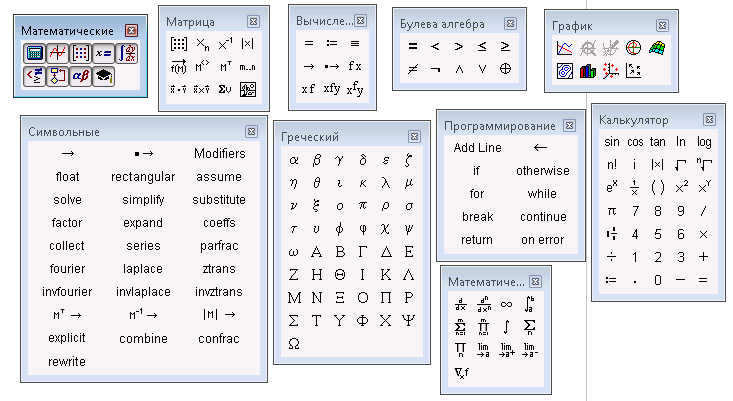
\includegraphics[width=\textwidth]{oldview.png}
	\end{center}
	\caption{Наборные панели пакета Mathcad} \label{fig:oldmathcad.view}
\end{figure}

По умолчанию ввод осуществляется в вычислительный блок. Для запуска формульного редактора достаточно установить курсор мыши в любом свободном месте окна редактирования и щелкнуть левой клавишей. Появится визир в виде маленького красного крестика. Его можно перемещать клавишами перемещения курсора. Визир указывает место, с которого можно начинать набор формул – вычислительных блоков. Подготовка вычислительных блоков облегчается благодаря выводу шаблона при задании того или иного оператора при помощи наборных панелей (см. рис. \ref{fig:oldmathcad.view}). Для ввода данных можно указать курсором мыши на нужный шаблон данных и щелчком левой ее клавиши ввести его.

Чтобы определить переменную, необходимо выполнить следующие действия:
\begin{itemize}
	\item набрать имя переменной (регистр имеет значение);
	\item ввести оператор присваивания «:=», сделать это можно нажатием кнопки «Определение» панели «Калькулятор» или «Вычисления» либо с помощью сочетания клавиш \keys{\shift+:};
	\item на место черного маркера, появившегося справа от оператора присваивания, ввести значение переменной.
\end{itemize}
Mathcad позволяет работать со следующими типами переменных:
\begin{itemize}
\item скалярная величина;
\item вектор (который также может быть задан с помощью оператора ранжированной переменной);
\item матрица.
\end{itemize}

Если переменная определяется как скалярная величина, то ее численное значение вводится с клавиатуры на место черного маркера. Работа в Mathcad осуществляется аналогично программированию на языках интерпретаторах, т.е. программа выполняется слева направо и сверху вниз. Это означает, что переменные должны быть определены в тексте программы левее или выше места их использования.

\primer{Используя формульный редактор, задайте переменную \mc{Data}, присвойте ей значение, целая часть которого --- день вашего рождения, десятичная --- месяц (например 1 января), и распечатайте ее экране используя оператор числового вычисления «=» на панели «Калькулятор»}:
\begin{figure}[h]
	\begin{center}
		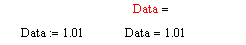
\includegraphics{oldz1.png}
	\end{center}
\end{figure}

Если распечатать переменную \mc{Data} левее и выше ее места определения и Mathcad выдаст ошибку.

\subsubsection*{Текстовый редактор}
Текстовый режим в Mathcad позволяет создавать всевозможные комментарии и качественно оформлять решенные задачи.
Чтобы ввести текстовую область, нажмите сочетание клавиш \keys{\shift+ ‘} (курсор ввода при этом должен располагаться на чистом участке документа). При этом появится специальная рамка, а курсор ввода приобретет вид красной вертикальной линии.
Набирается текст в Mathcad точно так же, как в любом текстовом редакторе. Если известно, сколько места на листе займет комментарий, то можно сразу растянуть текстовую область до нужных размеров. Чаще же текст просто вводят в область, обрывая строки с помощью клавиши \keys{\enter}, когда они достигают нужной длины (это приходится делать, так как Mathcad не выполняет автоматически переносов слов).

\primer{Сделайте шапку для документа: введя название лабораторной работы, номер группы и фамилию с инициалами:}

\begin{center}
	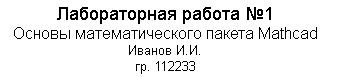
\includegraphics{oldz2.png}
\end{center}


\subsubsection{Массивы (векторы, матрицы)}
Массивы, по принципу задания их элементов, можно разделить на две группы:
\begin{itemize}
	\item векторы и матрицы, при задании которых не существует прямой связи между величиной элемента и его индексами;
	\item ранжированные переменные --- векторы, величина элементов которых напрямую определяется индексом.
\end{itemize}
В Mathcad реализовано несколько способов задания массивов:
\begin{itemize}
	\item задание матрицы или вектора вручную с помощью команды «Вставить матрицу»;
	\item определение матрицы последовательным заданием каждого элемента;
	\item  использование ранжированных переменных;
	\item создание таблицы данных;
	\item чтение из внешнего файла, и др.
\end{itemize}

Наиболее простым способом задания матрицы является использование специального окна «Вставить матрицу» (вызывается нажатием кнопки «Матрица или вектор» на наборной панели «Матрицы» или сочетанием клавиш \keys{\ctrl+M}). Параметры создаваемой матрицы или вектора можно определить в окошках «Строк» и «Столбцов». В результате в документ будет вставлена заготовка с черными маркерами вместо элементов, в которые необходимо ввести нужные значения:

\begin{center}
	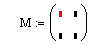
\includegraphics{oldz3-m.png}
\end{center}


Элементы матрицы могут быть как числами, так и выражениями. Если среди выражений или символов, выступающих в качестве элементов матрицы, есть неизвестные или параметры, то они обязательно должны быть численно определены выше. В противном случае матрица должна быть задана как функция.

\primer{Задайте вектор \mc{B}, содержащий три произвольных численных значения, и квадратную матрицу \mc{M}, содержащую девять произвольных значений, и распечатайте их:}

\begin{center}
	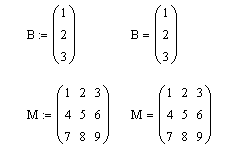
\includegraphics{oldz3.png}
\end{center}


В случае заданной матрицы всегда можно получить значение любого его элемента, используя его матричные индексы. Матричные индексы равняются номеру строки и столбца, на пересечении которых элемент находится. В математике отсчет строк и столбцов принято начинать с единицы. В программировании же начальные индексы обычно равняются нулю. По умолчанию в Mathcad строки и столбцы тоже начинаются с нуля. В том случае если такая система не удобна, то точку отсчета можно изменить на вкладке «Опции рабочего листа» (вкладка основного меню «Инструменты») изменив параметр «Начальный индекс» на единицу.

Итак, чтобы получить значение какого-то матричного элемента, нужно ввести имя матрицы с соответствующими индексами и поставить «=». Для задания индексов на панели «Матрицы» имеется специальная кнопка «Нижний индекс», которой соответствует клавиша \keys{[} . Нажав ее, вы увидите, что на месте будущего индекса, чуть ниже текста имени матрицы, появится черный маркер . В него через запятую следует ввести значения индексов. На первом месте при этом должен стоять номер строки, а на втором – номер столбца. При выделении элемента вектора нужно задать только индекс строки. Индексы также могут быть определены и через выражения или специальные функции.

Помимо одного элемента можно очень просто выделить и целые матричные столбцы. Чтобы это сделать, нужно использовать специальный оператор панели «Матрицы» «Столбец матрицы» (также вводится сочетанием  \keys{\ctrl + 6})  и в черный маркер ввести требуемый номер столбца. В том случае, если требуется выделить строку, матрицу необходимо транспонировать (оператор «Транспонирование матрицы» той же рабочей панели).

\primer{Обратитесь к центральному элементу матрицы М и распечатайте его значение. Обратитесь к первому столбцу матрицы М и распечатайте его значение. Обратитесь к второму элементу вектора В и распечатайте его значение. Измените начало отсчета векторов и матриц с 0 на 1 и повторите задание:}

\begin{center}
	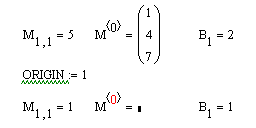
\includegraphics{oldz3-2.png}
\end{center}


При работе с массивами Mathcad воспринимает их как матрицы, поэтому при вычислениях будут применяться матричные операции (сложение, умножение и т.д.). Однако зачастую при расчетах матрицы используются для хранения однотипных данных, зависимостей. Поэтому в вычислениях необходимо использовать поэлементные операции, когда операции производятся над элементами с соответствующими индексами. Для осуществления поэлементных матричных операций на панели  «Матрица» есть кнопка векторизовать  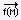
\includegraphics{oldz3-3.png}(сочетание клавиш \keys{\ctrl + -})

\primer{Задайте две квадратные матрицы \mc{A} и \mc{B} с произвольными значениями элементов. Найдите произведение матриц и поэлементное произведение элементов:}

\begin{center}
	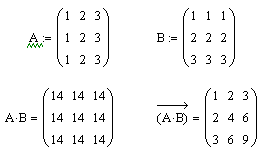
\includegraphics{oldz3-4.png}
\end{center}


\subsubsection*{Ранжированные переменные}
Одной из разновидностей задания массивов является использование так называемых ранжированных переменных. Ранжированная переменная – это разновидность вектора, особенностью которого является непосредственная связь между индексом элемента и его величиной. В Mathcad ранжированные переменные очень активно используются как аналог программных операторов цикла (например, при построении графиков).
Простейшим примером ранжированной переменной является вектор, значение элементов которого совпадает с их индексами. Для задания такой ранжированной переменной выполните следующую последовательность действий.
\begin{enumerate}
	\item Введите имя переменной и оператор присваивания.
	\item  Поставив курсор в маркер значения переменной, нажмите кнопку «Диапазон переменных» панели «Матрицы». При этом будет введена заготовка в виде двух маркеров, разделенных точками:
	\begin{figure}[h]
		\begin{center}
			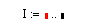
\includegraphics{oldz4-1.png}
		\end{center}
	\end{figure}
		
	Данную заготовку можно вставить с помощью клавиши \keys{;}.
	
	\item  В левый черный маркер заготовки ранжированной переменной введите ее первое значение, в правый – последнее.
\end{enumerate}

Шаг изменения ранжированной переменной при ее задании с помощью описанного способа постоянен и равен единице. Однако при необходимости его можно сделать и произвольным. Дли этого нужно, поставив после левой границы интервала запятую, ввести второе значение ранжированной переменной. Разность между первым и вторым ее значением и определит шаг. 
Использование ранжированных переменных во многом основано на том, что большинство математических действий в Mathcad над векторами осуществляется точно так же, как над простыми числами. Так, например, существует возможность вычисления значений практически любой встроенной и пользовательской функции от вектора. При этом в качестве результата будет выдан вектор, составленный из значений функции при величинах переменных, равных соответствующим элементам исходного вектора.

\primer{Задайте ранжированную переменную \mc{С} от 0 до 3 (шаг изменения переменной по умолчанию) и распечатайте ее значения. После задайте новый шаг изменения ранжированной переменной \mc{Е} (например 0.5) и распечатайте ее значения:}
\begin{figure}[h]
	\begin{center}
		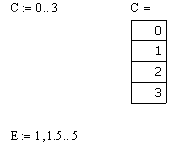
\includegraphics{oldz4-2.png}
	\end{center}
\end{figure}

\subsubsection*{Таблицы}
Все экспериментальные данные обрабатываются в Mathcad в виде матриц. Однако использовать описанные выше стандартные методы задания массивов для этого крайне неудобно. В этом случае можно использовать так называемую таблицу ввода. Чтобы ее вызвать, задействуйте команду \menu[,]{Вставить, Данные, Таблица} главного меню (соответствующая этой команде кнопка имеется и на панели «Стандартные»). В документ будет введена следующая заготовка:
\begin{figure}[h]
	\begin{center}
		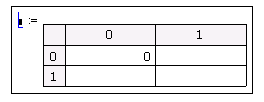
\includegraphics{oldz5-1.png}
	\end{center}
\end{figure}

Присвоив будущей матрице определенное имя (вводится в черный маркер слева от знака присваивания), попробуйте определиться с ее размерами. Если она не очень большая, можно сразу расширить пустую таблицу до нужной величины. Для этого следует использовать специальные черные маркеры, появляющиеся на контуре таблицы при ее выделении. Никаких ограничений на размеры таблица ввода не имеет. Создание таблицы повторяет заполнение обычных матриц, однако в таблицах нельзя использовать формулы.

Так как таблицы являются для Mathcad такими же матрицами, как заданные стандартными способами, с ними можно проводить все те же преобразования, что и со стандартными массивами. Если отобразить содержание таблицы через ее имя, оно визуализируется (при стандартных настройках) как простая матрица.

\primer{Задайте таблицу \mc{Т}, состоящую из 2 столбцов и 5 строк (нумерацию массивов начать с 0). Распечатать отдельно каждый столбец таблицы и один из элементов таблицы:}
\begin{figure}[h]
	\begin{center}
		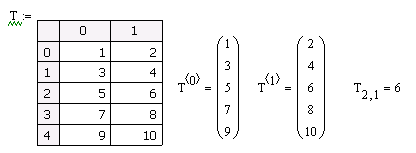
\includegraphics{oldz5-2.png}
	\end{center}
\end{figure}


\subsubsection{Операторы}
Операторы --- это символ или последовательность символов, обозначающих то или иное математическое действие. Операторы, выполняющие все основные арифметические действия, расположены на панели «Калькулятор» (рис. \ref{fig:oldmathcad.view}). Ввод основных арифметических операторов может быть также осуществлен с клавиатуры.

\subsubsection{Функции}
Функции в Mathcad делятся на две группы:
\begin{itemize}
\item функции пользователя;
\item встроенные функции.
\end{itemize}
Техника использования функций обоих типов абсолютно идентична, а вот задание отличается принципиально. Для задания функции пользователя необходимо выполнить следующие действия:
\begin{itemize}
\item ввести имя функции;
\item после имени ввести пару круглых скобок, в которых через запятую необходимо указать все переменные, от которых зависит функция;
\item ввести оператор присваивания «:=»;
\item на место черного маркера, появившегося справа от оператора присваивания, необходимо задать вид функции.
\end{itemize}

В выражение определяемой функции могут входить как непосредственно переменные, так и другие встроенные и пользовательские функции. 

Встроенные функции --- это функции, заданные в Mathcad изначально. Чтобы их использовать, достаточно корректно набрать имена функций с клавиатуры. Наиболее распространенные из них можно ввести с панели «Калькулятор», это синус, косинус, тангенс, натуральный и десятичный логарифмы, экспонента. Для того чтобы задать все остальные встроенные функций Mathcad, нужно открыть специальное окно «Вставить функции».

\primer{ Задайте пользовательскую функцию $y=x^2+x-1$, подставьте в качестве аргумента ранее определенные переменные \mc{Data} и \mc{С}, а также выражение \mc{2 Data}:}
\begin{figure}[h]
	\begin{center}
		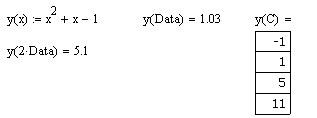
\includegraphics{oldz6-1.png}
	\end{center}
\end{figure}

\primer{Задайте пользовательскую функцию $y(x)=\dfrac{x^2 +\cos(x)}{2}$, 
подставьте в качестве аргумента ранее определенные переменные \mc{Date} и \mc{С}:}
\begin{figure}[h]
	\begin{center}
		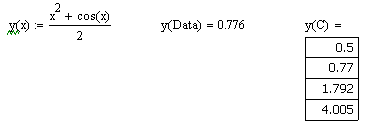
\includegraphics{oldz6-2.png}
	\end{center}
\end{figure}

\subsubsection{Графический редактор}
Все основные типы графиков и инструменты работы с ними расположены на рабочей панели «Графики» (рис. \ref{fig:oldmathcad.view}). Здесь можно найти ссылки на семь типов графиков. В курсе математического моделирования потребуются только график кривой в двумерной декартовой системе координат. Соответствующая графическая заготовка вызывается из наборной панели «Графики» -Y график 
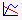
\includegraphics{oldz7-1.png}:
\begin{figure}[h]
	\begin{center}
		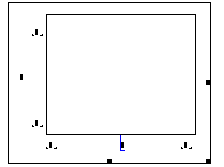
\includegraphics{oldz7-2.png}
	\end{center}
\end{figure}

На рисунке область ввода значения аргумента и функции обозначена черными метками по центру соответствующих осей. По оси абсцисс откладывается аргумент, например \mc{x}, по оси ординат функция -- например \mc{y(x)}. Границы по осям выставляются автоматически, но предусмотрено их изменение вручную. Переход к редактированию осуществляется постановкой курсора в соответствующий регистр по осям абсцисс и ординат, на рисунке это черные метки в начале и конце каждой оси, отмеченные по краям снизу черными угловыми линиями.

В ряде случаев (например, если в графике приходится очень часто менять диапазоны по осям или необходимо выделить конкретную область) можно задать векторы данных самостоятельно. Сделать это можно с помощью оператора ранжированной переменной (задание ранжированной переменной рассматривалось выше). В этом случае аргумент функции задается в виде вектора, т.е. переменная и функция будут заданы в виде двух соразмерных векторов, по которым будет построен график.

Mathcad позволяет отображать до 16 графических зависимостей в одной системе координат, что удобно для визуального контроля и сравнения полученных результатов. Чтобы добавить к уже имеющемуся графику еще один, выполните следующую последовательность действий:
\begin{itemize}
	\item Установите курсор справа от выражения, определяющего координаты последнего ряда данных по оси \mc{y} (предварительно выделив его).
	\item Нажмите клавишу \keys{,}. При этом курсор опустится на строку ниже и появится чистый маркер.
	\item В появившийся маркер введите выражение для новой функции или имя функции.
\end{itemize}

С помощью описанного метода можно построить графики функций одной переменной. Если же кривые, которые нужно отобразить на одной области, зависят от различных переменных, то их, аналогично добавлению новых функций, следует ввести через запятую в нижний маркер в том же порядке, что и соответствующие им функции.

Изменение настроек отображения осей и графиков (если необходимо изменить тип или цвет кривой) осуществляется с помощью диалогового окна «Форматирование выбранной декартовой плоскости», вызвать которое можно, дважды щелкнув левой кнопкой мыши на области графика.

\primer{Постройте графическую зависимость для функции \mc{y(x)}, определенной в предыдущем задании и функции $5 \sin(x)$. Измените диапазон графика путем определения аргумента как ранжированной переменной от 0 до 5. Посмотрите как шаг ранжированной переменной влияет на график:}

\begin{center}
	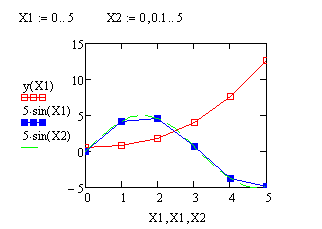
\includegraphics{oldz8-1.png}
\end{center}


\subsubsection*{Символьные вычисления}
В Mathcad имеет возможности символьных вычислений: решение уравнений, преобразования, разложения и т.д. Для аналитического преобразования можно воспользоваться кнопкой 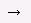
\includegraphics{oldz11-1.png} на панели «Символьные вычисления» или сочетанием \keys{\ctrl + .}
\primer{Вычислите производную и интеграл выражения $x^2+\sin(x)$}
\begin{figure}[h]
	\begin{center}
		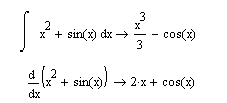
\includegraphics{oldz11-2.png}
	\end{center}
\end{figure}

\subsubsection*{Численное решение уравнений и систем уравнений}
Для численного поиска решений уравнений с одним неизвестным в Mathcad существует специальная встроенная функция \mc{root}. Функция эта может использоваться в двух различных формах, при этом реализуются разные численные алгоритмы. Так, если определена только одна точка приближения к корню, поиск решений будет осуществляться методом секущих. Если же задан интервал, на котором предположительно локализовано решение, то поиск его будет осуществлен с применением двух модификаций метода бисекции.

Если необходимо найти корень некоторого уравнения, причем известен интервал, в котором он локализован, проще всего использовать функцию с четырьмя аргументами: \mc{rоot(f(x), x, a, b)}, где \mc{f(x)} --- функция, определяющая уравнение, \mc{х} --- переменная, \mc{a} и \mc{b} --- границы интервала локализации. Обязательным условием является то, что значения функции на концах интервала должны быть противоположных знаков. Это связано с особенностью используемых \mc{root} алгоритмов. Если нарушить это условие, система выдаст сообщение об ошибке.


В тех случаях, когда определить границы такой локализации невозможно, следует применять функцию \mc{root} с одной точкой приближения: \mc{rоot(f(x),x)}. В этом случае необходимо перед вызовом функцию \mc{root} задать для переменной \mc{x} начальное приближение.

Важной характеристикой решения является его точность. В Mathcad можно регулировать величину погрешности решения, изменяя значение специальной системной переменной \mc{TOL}. В общем случае, чем меньше \mc{TOL}, тем точнее будет найден корень, но и тем больше времени уйдет на его определение (а также будет выше риск, что численный метод не сойдется к решению).

\primer{Найти с помощью функции \mc{root} корни уравнения: $x^3-10 x +2 =0$
	используя различные интервалы локализации и точки начального приближения:}
\begin{figure}[h]
	\begin{center}
		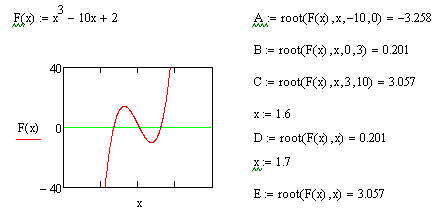
\includegraphics{oldz9-1.png}
	\end{center}
\end{figure}

Для численного решения систем уравнений в Mathcad служит блок \mc{Given-Find}. Используя блок \mc{Given-Find}, можно решать системы, содержащие до 250 нелинейных уравнений и до 1000 линейных. Результатом решения системы будет численное значение искомых корней.


Для решения системы уравнений с помощью блока \mc{Given - Find} необходимо выполнить следующее:
\begin{itemize}
	\item Задайте начальные приближения для всех неизвестных, входящих в систему уравнений. Mathcad решает уравнения при помощи итерационных методов. На основе начального приближения строится последовательность, сходящаяся к искомому решению. 
	\item Напечатайте в рабочем окне Mathcad ключевое слово \mc{Given}. Оно указывает Mathcad, что далее следует система уравнений.
	\item Введите уравнения и неравенства в любом порядке ниже ключевого слова \mc{Given}. В качестве знаков равенства следует использовать логическое равенство . Ввести его можно нажатием кнопки «Булево равенство» панели «Булева алгебра» либо с помощью сочетания клавиш \keys{\ctrl+ =}. Между левыми и правыми частями неравенств может стоять любой из логических символов $<$, $>$, $\leqslant$ и $\geqslant$ (панель «Булева алгебра»).
	\item Введите функцию решения систем уравнений \mc{Find}{$\mathrm{(x_1, x_2)}$} и оператор численного вывода (знак «=»). В скобках через запятую задайте переменные в том порядке, в котором должны быть расположены в ответе соответствующие им корни. Если результаты решения требуется использовать в дальнейших расчетах, то тогда их необходимо присвоить некоторой переменной \mc{Z:=Find}{$\mathrm{(x_1, x_2)}$}.
\end{itemize}

\primer{Решите систему нелинейных уравнений $\sqrt{x}+\sqrt{y}=9$, и $\sqrt[3]{x}+ \sqrt[3]{y}=5$ выведите результат на печать:}

\begin{center}
	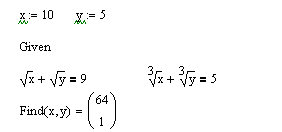
\includegraphics{oldz9-2.png}
\end{center}



Вопросы для самоконтроля
\begin{enumerate}
	\item Для каких целей предназначен математический пакет Mathcad?
	\item С какими типами переменных позволяет работать Mathcad?
	\item В чем разница между оператором присваивания и оператором численного решения?
	\item Какие типы функций есть в Mathcad, в чем их отличие?
	\item  Для чего предназначен графический редактор?
	\item Для чего предназначен текстовый редактор?
\end{enumerate}
		\laborator{Регрессионный анализ, методы аппроксимации}

\goal ознакомиться с возможностями математического пакета Mathcad при решении задач регрессионного анализа; ознакомиться с процедурами численного решения алгебраических уравнений и систем уравнений, реализованными в данном пакете. 

\subsubsection*{Теория}
Регрессионный анализ --- статистический метод исследования зависимости между зависимой переменной $y$ и одной или несколькими независимыми переменными $x_1$, $x_2$, $...$, $x_n$.
В статистике для оценки силы корреляционной зависимости двух случайных величин используется коэффициент корреляции $r_{xy}$. Определяется он отношением математического ожидания произведения отклонений случайных величин от их средних значений к произведению среднеквадратичных отклонений этих величин:
\begin{equation}
r_{xy}=\dfrac{\dfrac{1}{n} \sum\limits_{i=1}^{n} (x_i-\bar{x}) (y_i-\bar{y}), }{\sigma_x \sigma_y}
\end{equation}
где $\sigma_x$ и $\sigma_y$ --- среднеквадратичные отклонения, определяемые следующим образом:
\begin{equation}
\sigma_x=\sqrt{\dfrac{1}{n} \sum\limits_{i=1}^{n}(x_i-\bar{x})^2},
\end{equation}
где $\bar{x}=\dfrac{1}{n} \sum\limits_{i=1}^{n} x_i$.
Аналогичные выражения записываются и для $y$.

В Mathcad коэффициент корреляции двух выборок по данной формуле можно подсчитать с помощью встроенной функции \mc{corr (x,y)} (где \mc{x} и \mc{y} --- векторы, между которыми определяется коэффициент корреляции). Если коэффициент корреляции равен по модулю единице, то между случайными величинами существует линейная зависимость. Если же он равен нулю, то случайные величины независимы. В случае промежуточных значений $r_{ху}$, зависимость $y$ от $x$ может быть нелинейной или иметь высокое значение шума.

Если две выборки коррелируют, то можно установить зависимость между ними. Для проведения регрессионного анализа в Mathcad имеется ряд функций. Конечный результат регрессионного анализа --- получение функции с набором параметров, с помощью которой можно оценить значения в промежутках между заданными точками. Расхождение полученной функции регрессии с экспериментальными данными можно оценить через относительную среднюю и максимальную ошибку:

\begin{equation}
err_i= \dfrac{\left| y_i^э - y(x^э_i) \right|}{y_i^э} 100\ \% ,
\end{equation}
\begin{equation}
err_{av}=\dfrac{1}{n}\sum\limits_{i=1}^{n} err_i ,
\end{equation}
где $y_i^э$, $y(x_i^э)$ --- экспериментальное и расчетное значения функции; $n$ --- число экспериментальных точек; $err_i$ --- ошибка в i–й точке (из них определяется максимальная); $err_{av}$ --- средняя ошибка функции регрессии.

В Mathcad имеются встроенные функции для определения среднего и максимального значения массива: \mc{mean(S)} находит среднее значение элементов матрицы \mc{S}, \mc{max(S)} --- максимальное значение.

\subsubsection{Линейная регрессия}
Линейная функция $y=ax + b $ является одной из наиболее простых и часто применяется для описания экспериментальных данных. 
Если поместить значения $x$ в вектор \mc{VX} и соответствующие значения $y$ в \mc{VY}, то линейная функция определяется в виде:
\mc{Y = slope(VX, VY) $\cdot$ X + intercept(VX, VY)},
где \mc{slope(VX, VY)} --- возвращает скаляр: тангенс угла наклона линии регрессии для данных из \mc{VX} и \mc{VY} (параметр $a$);
\mc{intercept(VX, VY)} - возвращает скаляр: смещение по оси ординат линии регрессии для данных из \mc{VX} и \mc{VY} (параметр $b$).

%Пример решения
\primer{Задайте экспериментальные данные, близкие к линейной зависимости, в виде таблицы. Определите коэффициент корреляции. Получите функцию линейной регрессии, описывающую эти экспериментальные данные. Графически и численно определите точность полученной функции регрессии.}

\begin{center}
	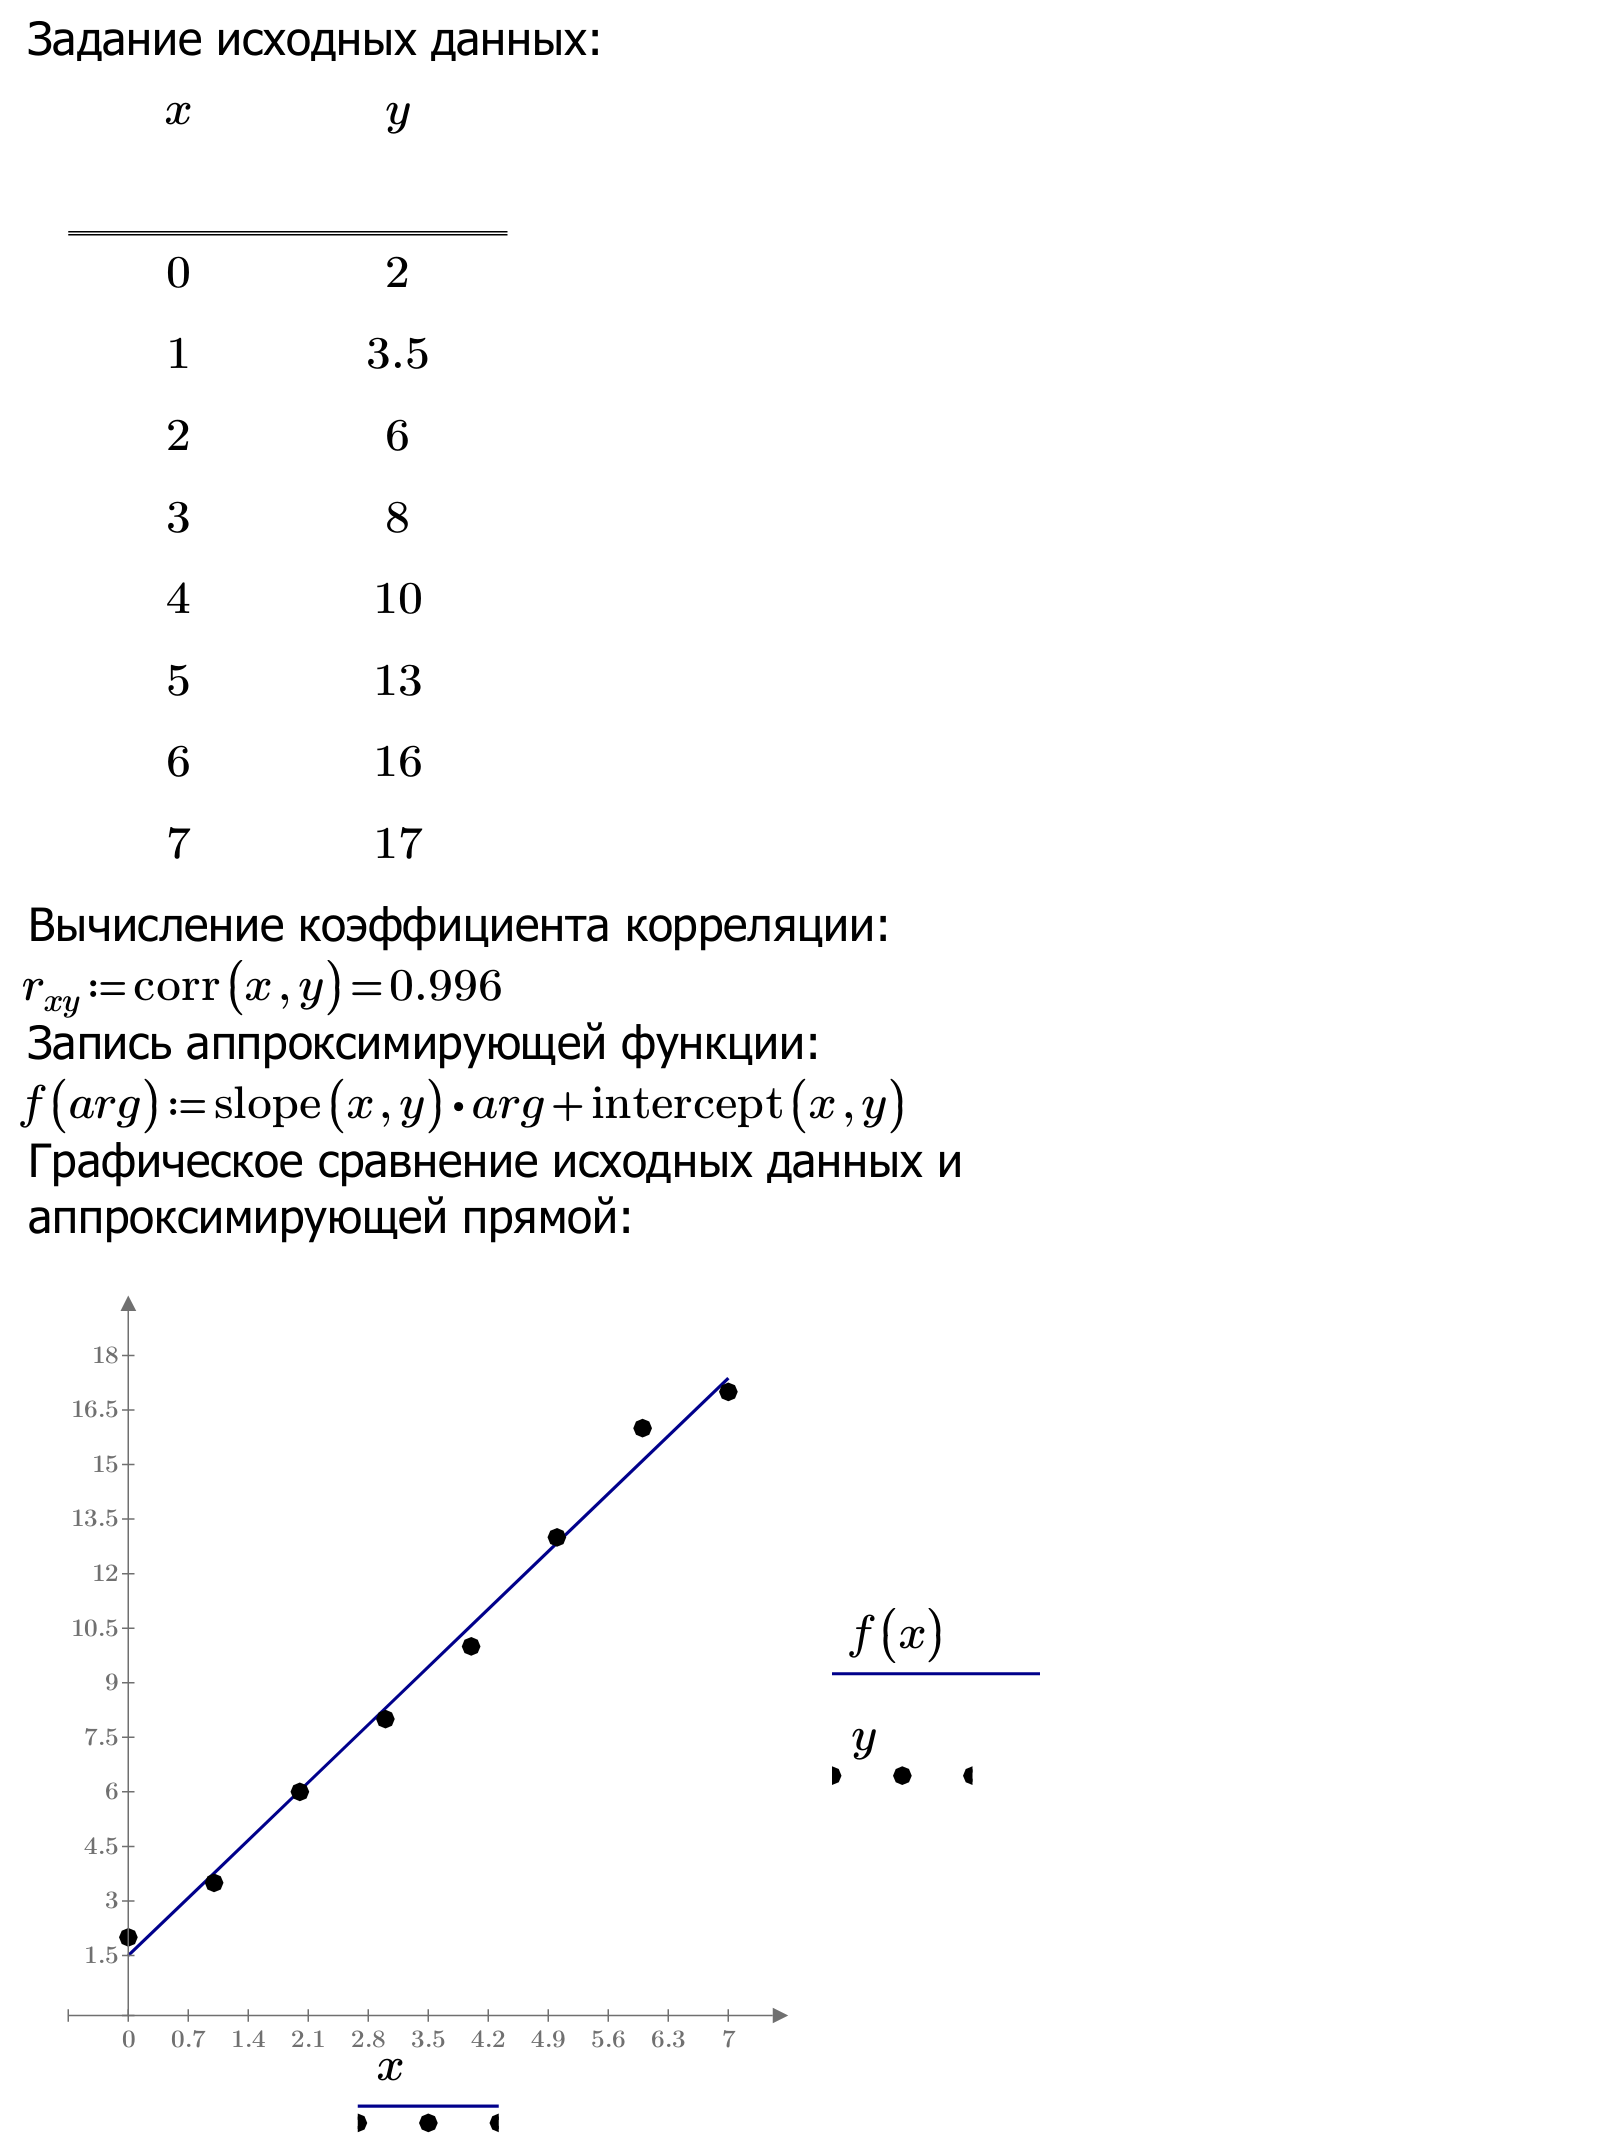
\includegraphics[scale=1.0]{new-regress-1-1.png}
\end{center}
\begin{center}
	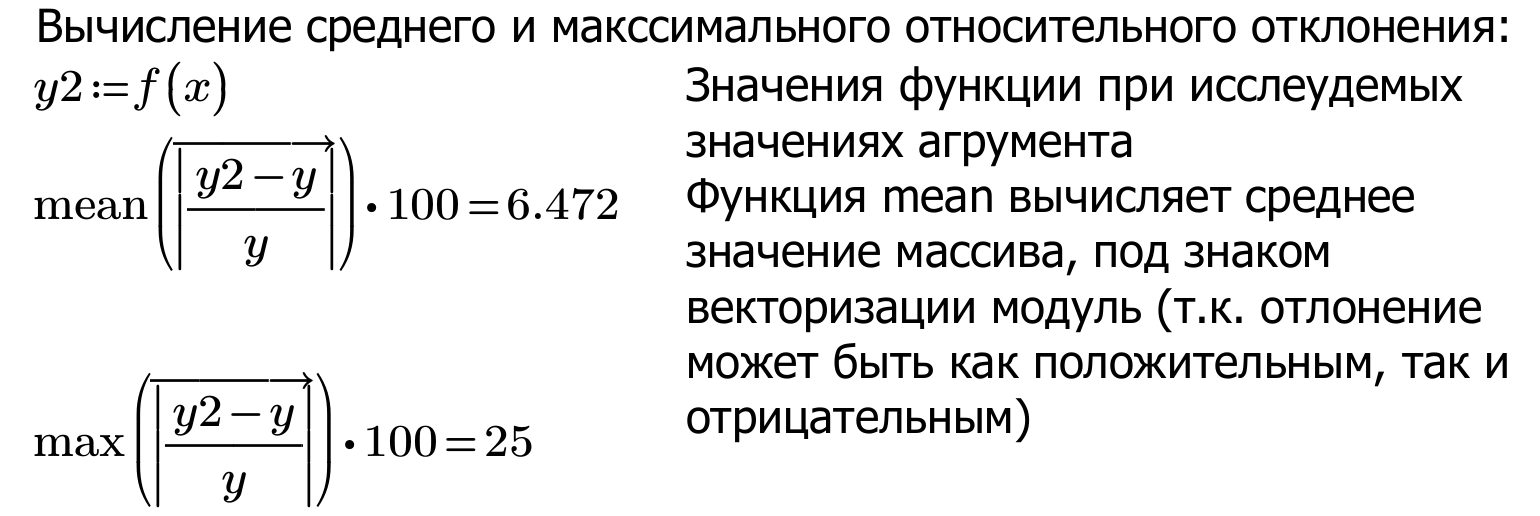
\includegraphics[scale=1.0]{new-regress-1-2.png}
\end{center}

\subsubsection{Полином}
Одной из  часто применяемых при обработке экспериментальных данных функций, является полиномиальная:
\begin{equation}
y(x)= \sum_{i=0}^{n} a_i x^i
\end{equation}
где $a$ --- параметры полинома, $n$ --- степень полинома. Для определения параметров полиномов используется функция \mc{regress}, которая допускает использование полинома любого порядка. Однако на практике не следует использовать степень полинома выше $n = 4$. Так как функция \mc{regress} пытается приблизить все точки данных, при недостаточном количестве экспериментальных данных высокая степень полинома может дать физически неадекватное поведение результирующей функции.

\mc{regress(vx, vy, n)} --- функция, определяющая параметры полином порядка \mc{n}, \mc{vx} и \mc{vy} --- m-мерные векторы, содержащие значения $x$ и $y$. Функция \mc{regress} возвращает вектор, содержащий кроме самих значений параметров полинома $a$ множество технической информации. Для того, чтобы вычислить значение полинома в какой-либо, точке используется функция: \mc{interp (vs, vx, vy, x)} --- возвращает интерполируемое значение $y$, соответствующее $x$.

\primer{Задайте экспериментальные данные в виде таблицы. Определите коэффициент корреляции. На основе этих данных получите функцию полиномиальной регрессии, описывающую экспериментальные данные. Графически и численно определите точность полученной функции регрессии.}

\begin{center}
	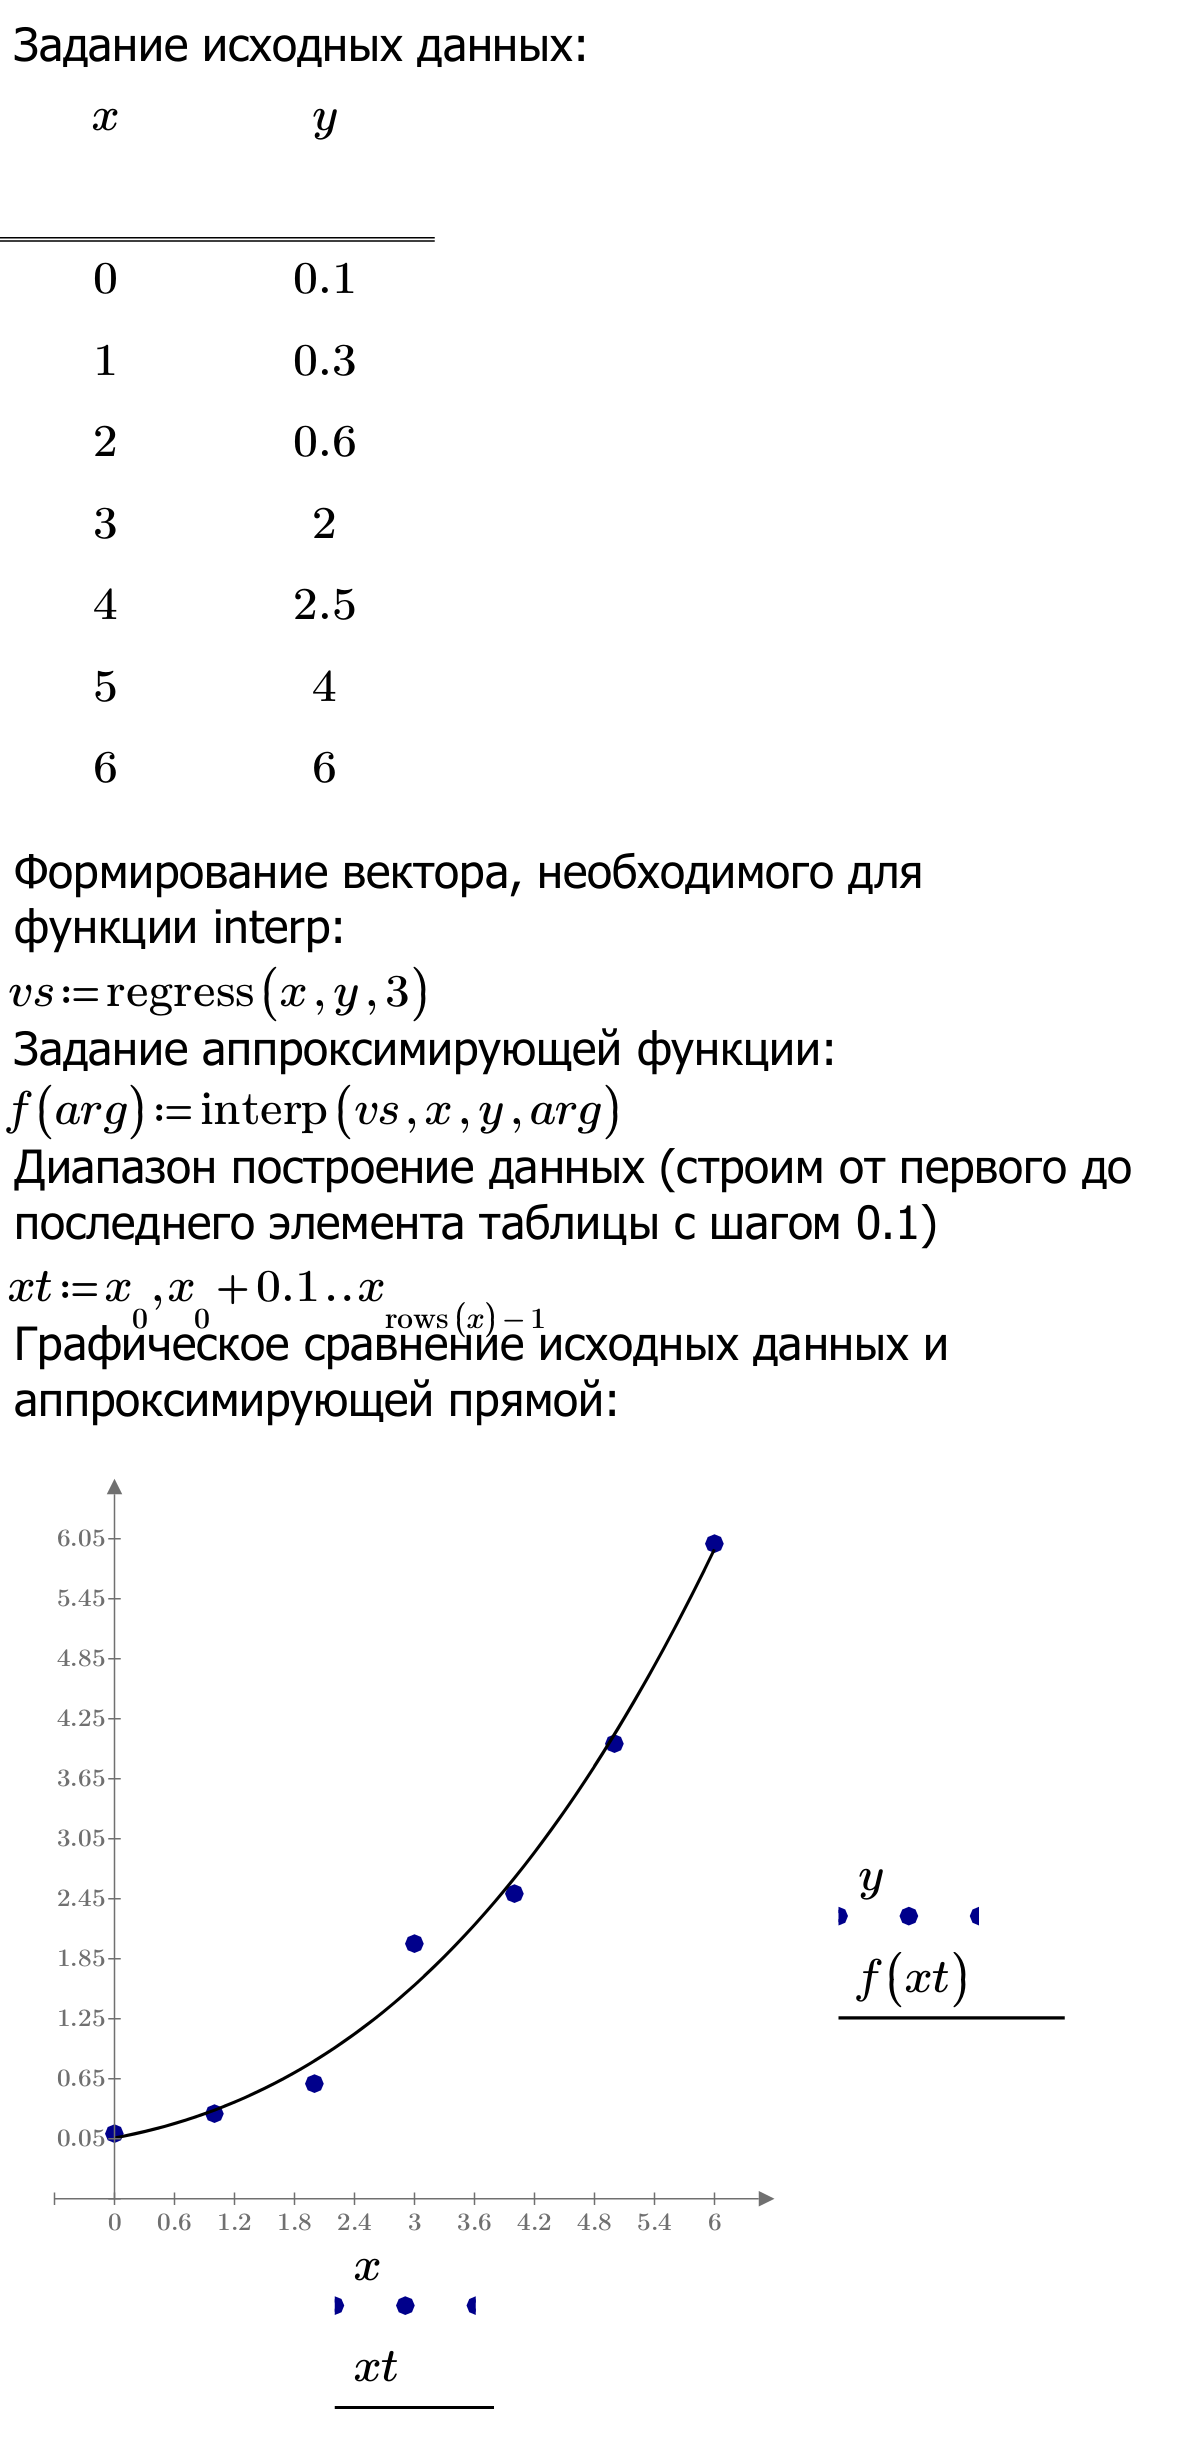
\includegraphics{new-regress-2.png}
\end{center}


\subsubsection{Обобщенная линейная регрессия (линейные по параметрам функции)}
Обобщенная линейная регрессия --- зависимость в виде линейных комбинаций произвольных функций, ни одна из которых не является полиномом.
Задача обобщенной линейной регрессии --- найти, какие значения должны принимать параметры $a_0, a_1, ..., a_N$, чтобы функция  $F(x)=a_0 f_0(x)+a_1 f_1(x)+ ... + a_N f_N(x)$, являющаяся линейным сочетанием $N+1$ произвольной функции $f_i(x)$, проходила между экспериментальными точками так, чтобы сумма квадратов расстояний от точек до кривой $F(x)$ была минимальной.

В Mathcad для вычисления параметров обобщенной линейной регрессии служит встроенная функция \mc{linfit(x, y, F)}, где \mc{x} и \mc{y} --- векторы экспериментальных данных, \mc{F} --- векторная функция, содержащая в качестве элементов функции, входящие в линейное сочетание.

\primer{Задайте произвольный набор данных $y$ и $x$. С помощью функции \mc{linfit} определите вид линейной зависимости между $y$ и $x$. В качестве функции используйте выражение
	$F(x)=a_0 \sin(x) + a_1 \cos(2x)+a_2 \sqrt[3]{x} + a_3 x$.}
%пример решения

\begin{center}
	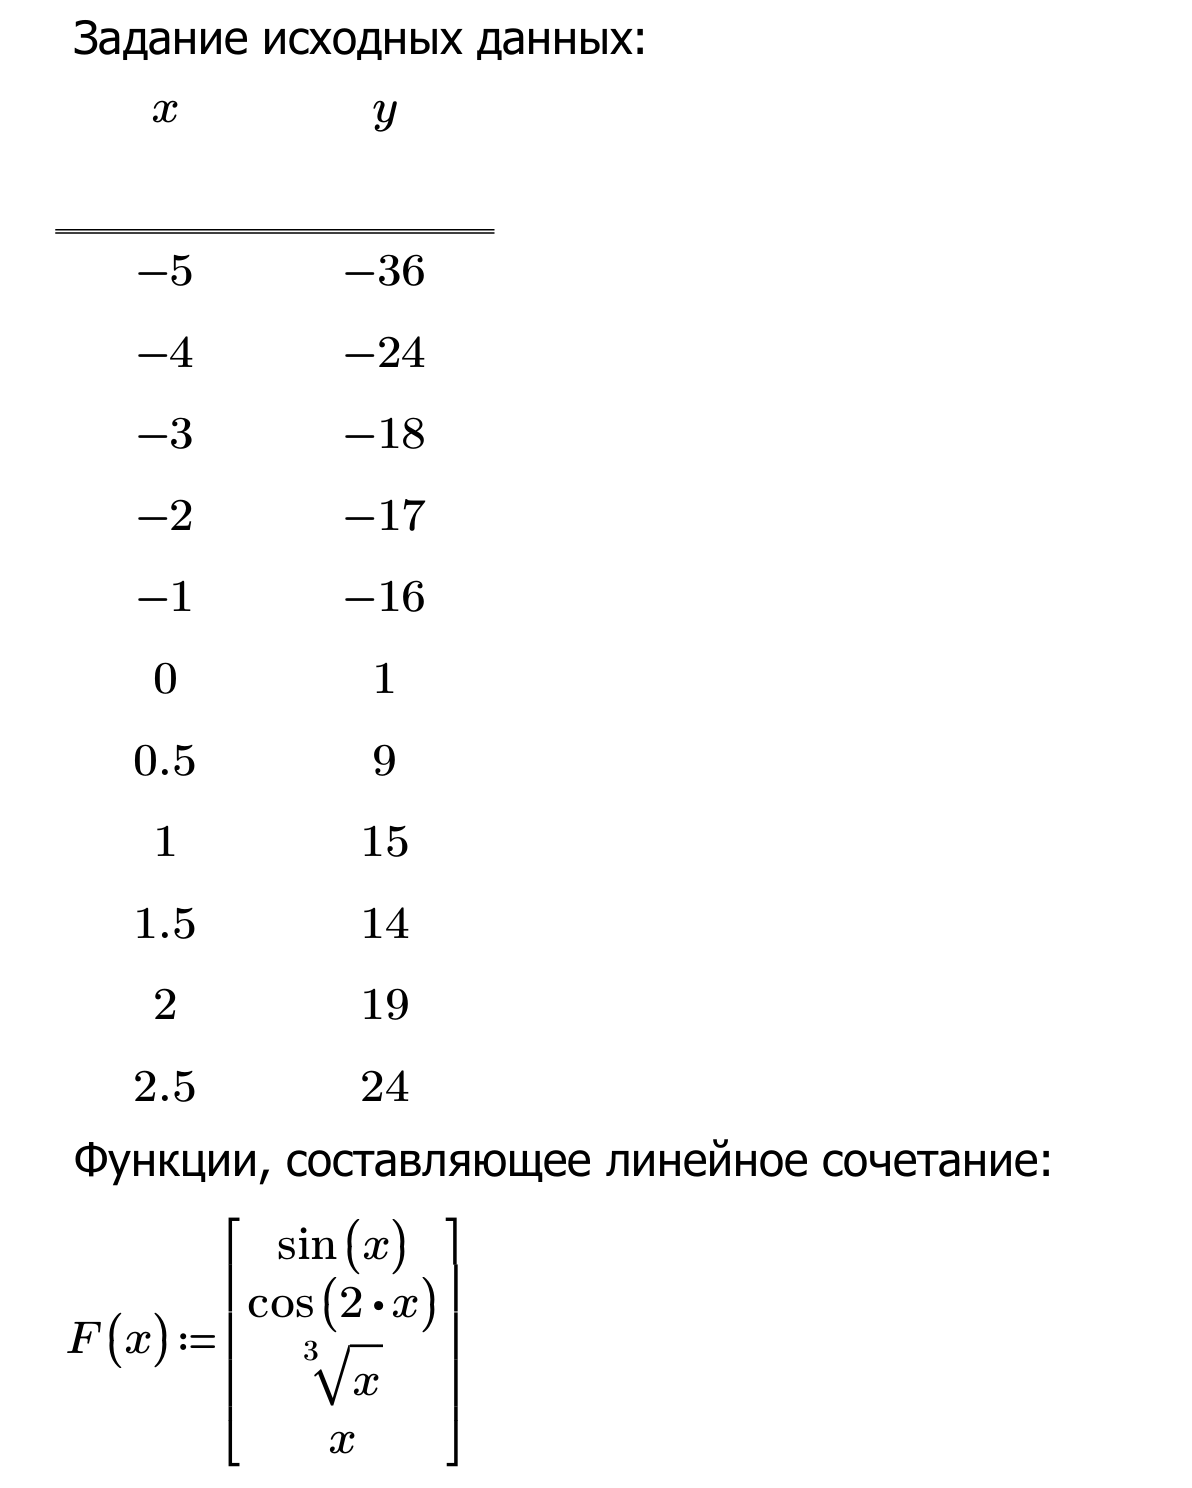
\includegraphics{new-regress-3-1.png}
\end{center}
\begin{center}
	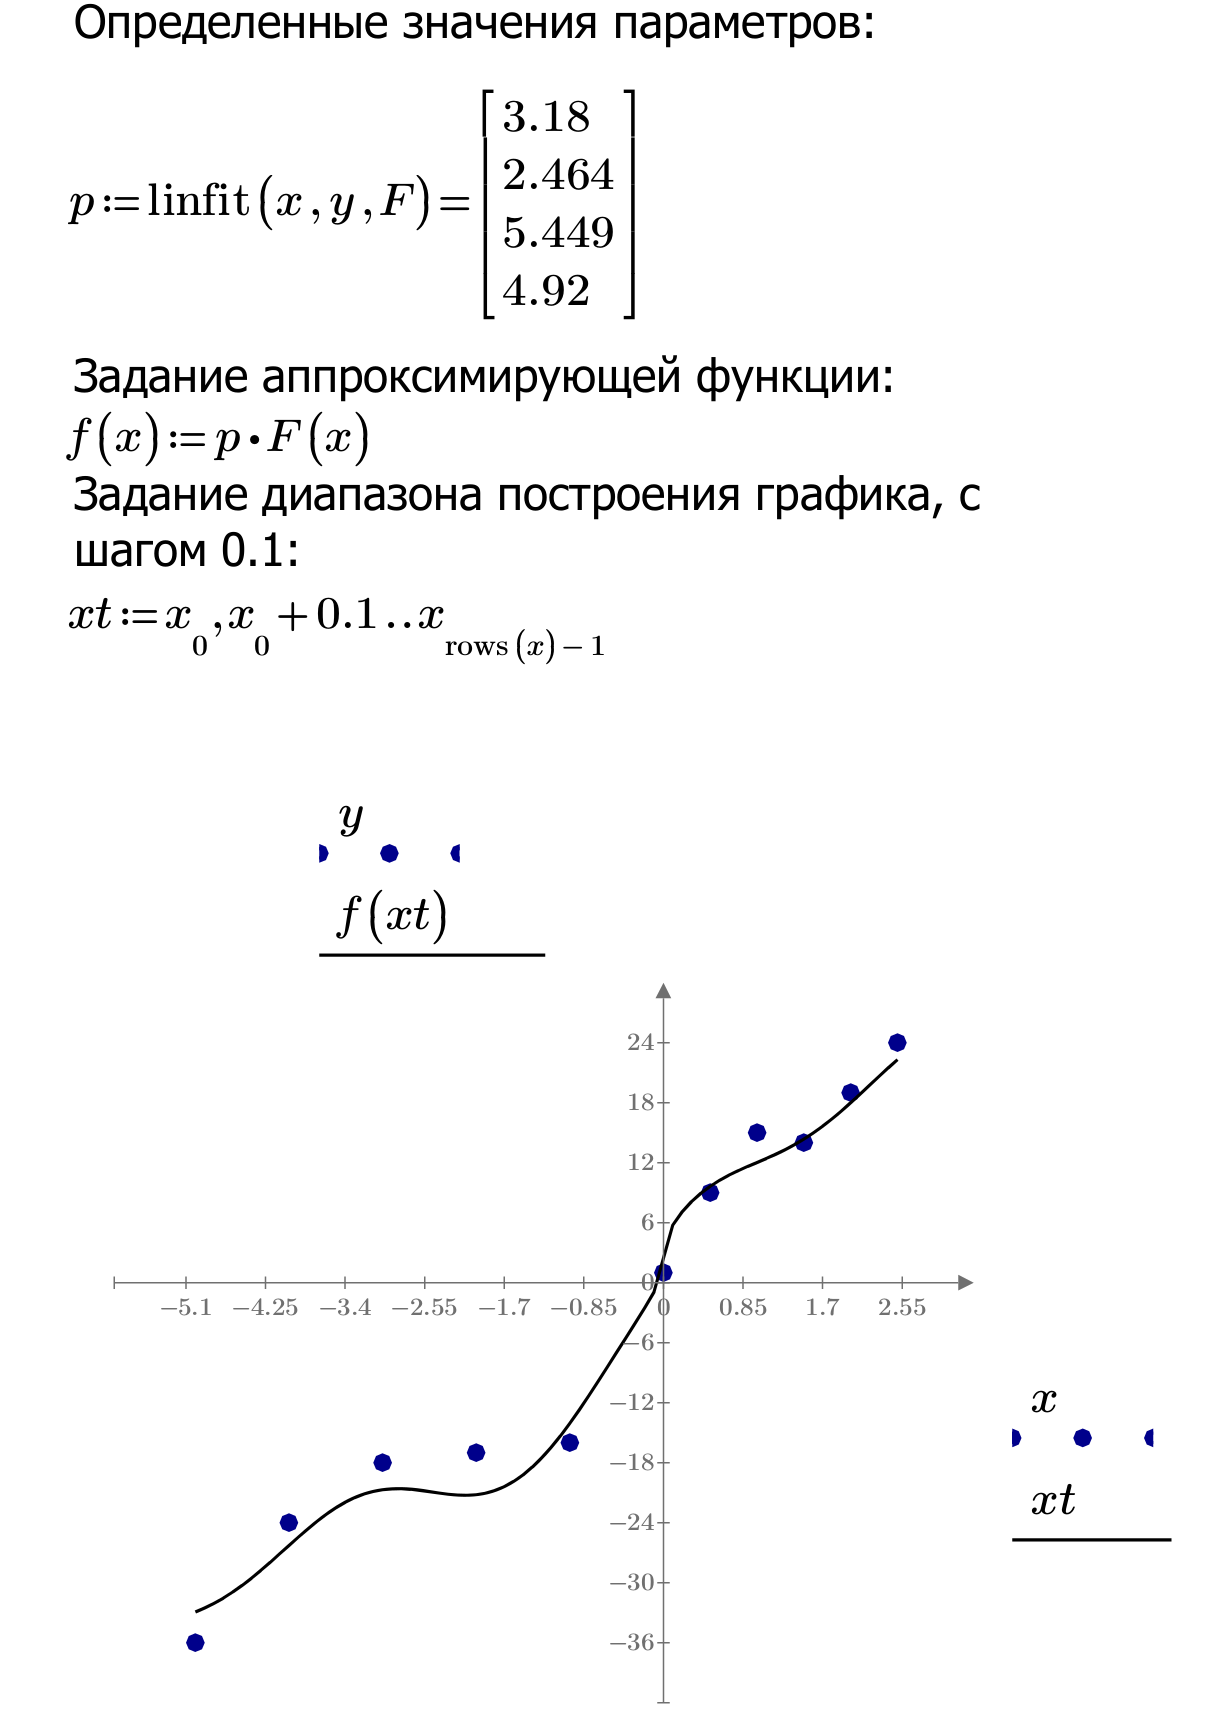
\includegraphics{new-regress-3-2.png}
\end{center}


\subsubsection{Нелинейная регрессия (нелинейные по параметрам функции)}

Если аппроксимирующая исходные данные функция представляется в виде $F(x) = f_0 (a_0, x) + f_1(a_1,x) +... + f_N(a_N,x)$, когда искомые коэффициенты $a_0, a_1, ..., a_N$ входят в функции, зависимость будет уже нелинейной по параметрам, соответственно функция \mc{linfit} уже не подойдет.
В Mathcad заложены зависимости наиболее распространенных нелинейных функций: синуса, экспоненты или др. Параметры для этих нелинейных зависимостей определяются функциями: 
\begin{itemize}
	\item \mc{expfit(x, y, g)} --- регрессия  экспоненциальной функцией $y(x)=a e^{b x}+c$;
	\item \mc{lgsfit(x, y, g)} --- регрессия логистической функцией $y(x)=a/(1+b e^{-c x})$;
	\item \mc{sinfit(x, y, g)} --- синусоидальная регрессия $y(x)=a sin(x+b)+c$;
	\item \mc{pwrfit(x, y, g)} --- регрессия степенной функцией $y(x)=a x^b+c$;
	\item \mc{logfit(x, y, g)} --- регрессия логарифмической функцией $y(x)=a\ln(x+b)+c$;
\end{itemize}
где \mc{g} --- вектор начальных приближений для поиска параметров. 

В случае, если используется какая~-либо произвольная нелинейная регрессия,  в Mathcad есть встроенная функция \mc{genfit(x, y, g, F)}. В качестве аргументов данная функция принимает следующие параметры: \mc{x}, \mc{y} --- вектор экспериментальных данных; \mc{g} --- вектор начальных приближений для неизвестных параметров;
\mc{F(x, A)} --- описывающая экспериментальную зависимость функция, параметры \mc{A} которой должны быть определены.

Параметры \mc{x} и \mc{y} приведенных функций соответствуют векторам координат исходных эмпирических данных. В переменной \mc{g} содержится вектор начальных приближений искомых параметров \mc{(a, b, c)}. Для определения параметров нелинейных по параметрам функций используются различные алгоритмы (например Левенберга~--Марквардта, градиентного спуска и т.д.) данные алгоритмы основаны на использовании каких-либо значений для параметров на первой итерации поиска.
Из всех встроенных функций регрессии \mc{genfit} является наиболее универсальной и может быть использована для любых функций. Однако для нелинейных по параметрам функций огромное влияние на точность расчета оказывает начальное приближение  \mc{g} для искомых параметров. Поэтому при возможности лучше ввести задачу к  использованию линейных по параметрам функции.

\primer{Задайте произвольный набор данных \mc{x} и \mc{y} в виде таблицы. Определите коэффициент корреляции между данными. Для аппроксимации данных используете функцию вида $y(x)=\exp(A+Bx+Cx^2)$ где $A$, $B$, $C$ --- параметры. Оценить точность полученной регрессии.}
%пример решения

\begin{center}
	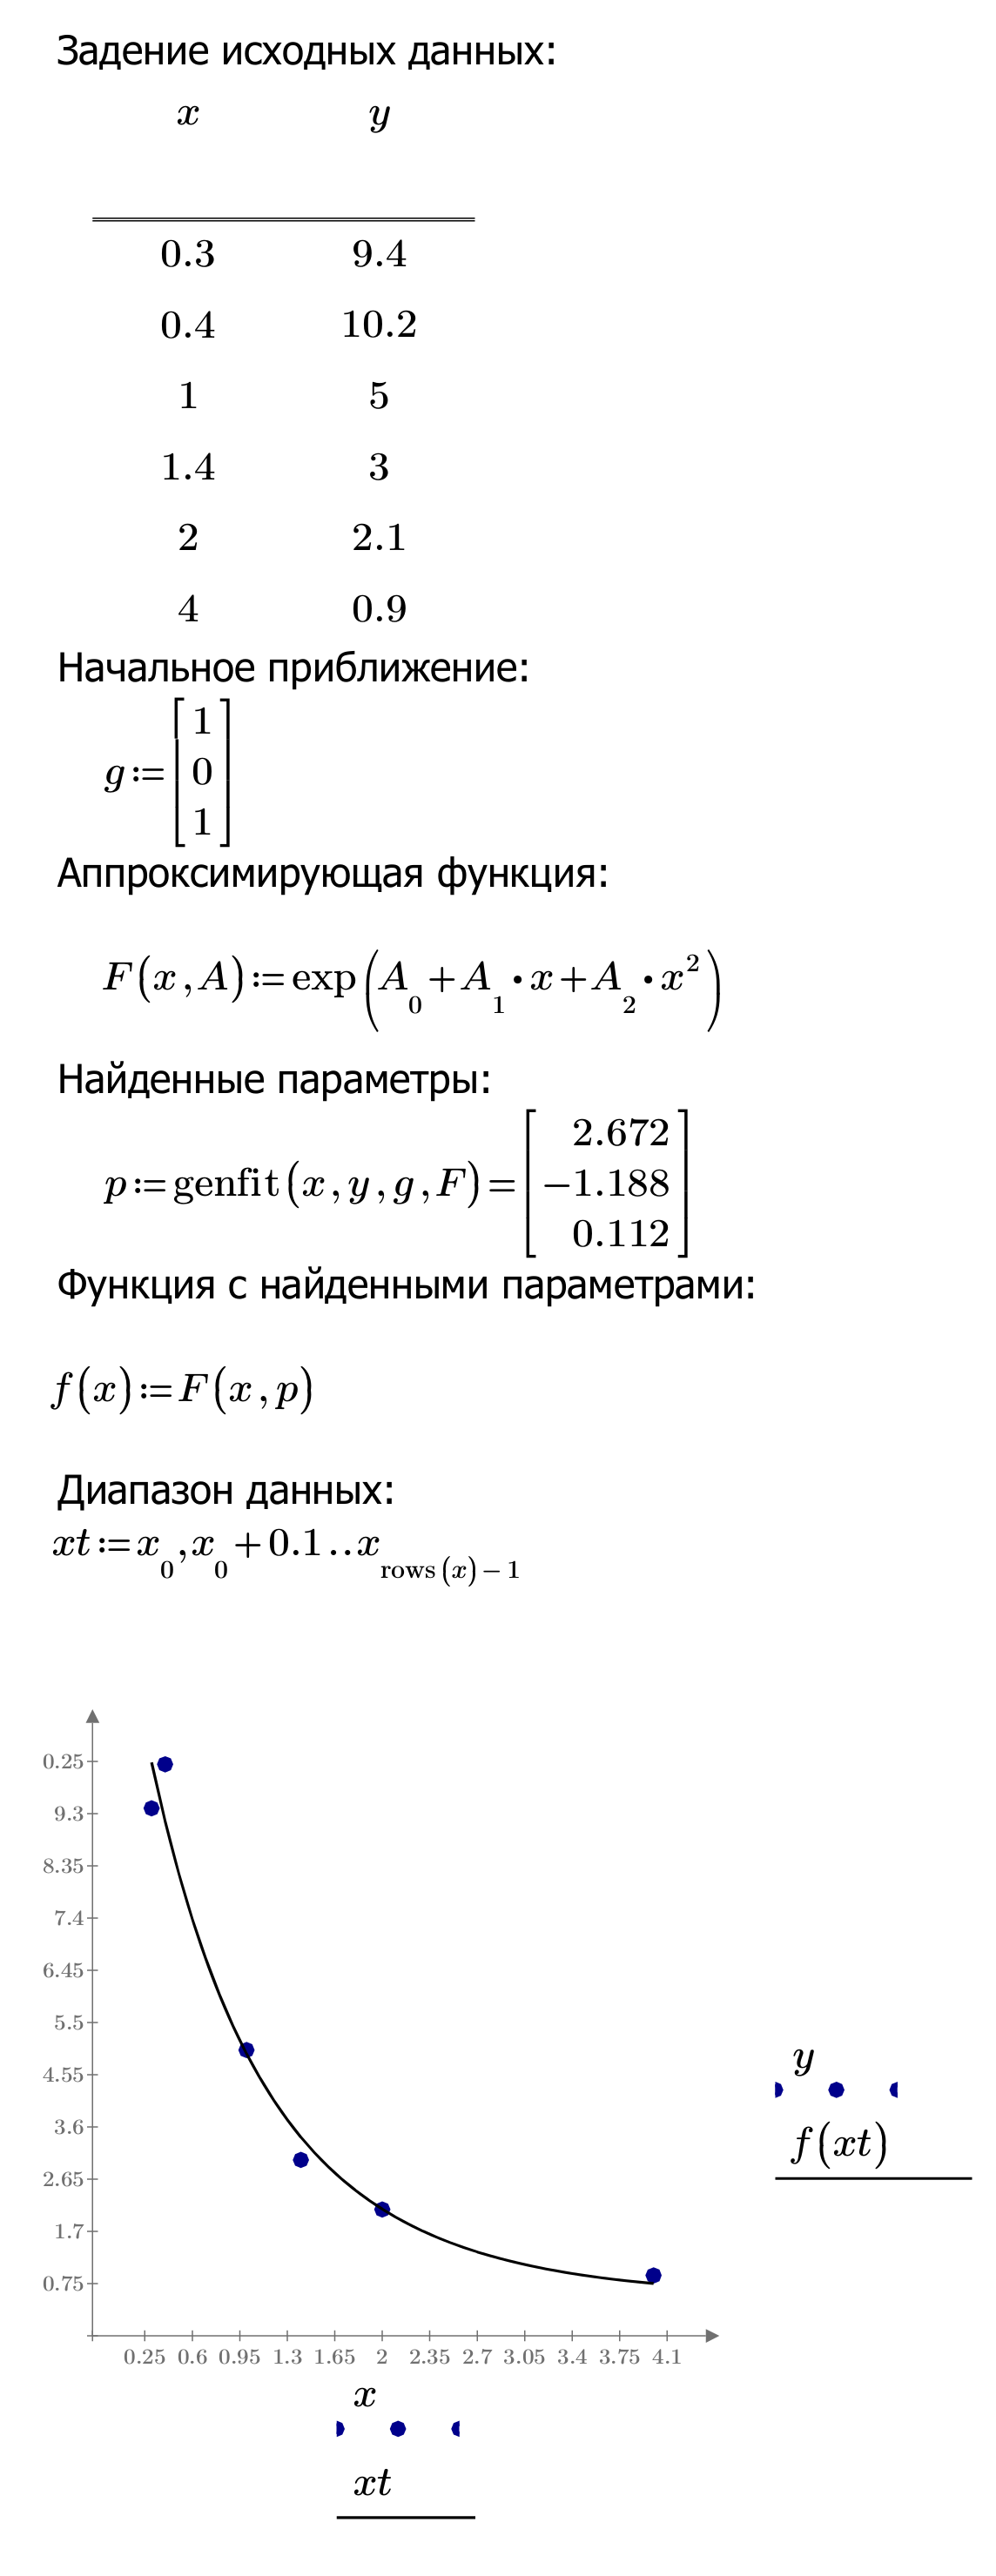
\includegraphics{new-regress-4.png}
\end{center}

В случае обработки точных данных, представленных в дискретном виде удобнее использовать сплайны. Сплайн представляет из себя кусочную функцию, составленную из полиномов какой-либо степени. Границы использования полиномов начинаются и заканчиваются строго во введенных значениях точек $x$ и $y$ (рисунок \ref{fig:old.regress.spline}). Также параметры полиномов настраиваются таким образом, что производная двух полиномов с каждой из сторон подходящих к точке будет одинаковой.
Таким образом два этих условия обеспечивают непрерывность и гладкость (непрерывность производной) сплайна. Однако сплайны неприемлемо применять для аппроксимации экспериментальных данных в связи с тем, что погрешности эксперимента будут вносить существенное влияние на результирующую функцию. В представленных лабораторных работах сплайн аппроксимации могут быть использованы при обработке численных решений дифференциальных уравнений.

\begin{figure}[h] %{0.6\textwidth}
	\begin{center} 
		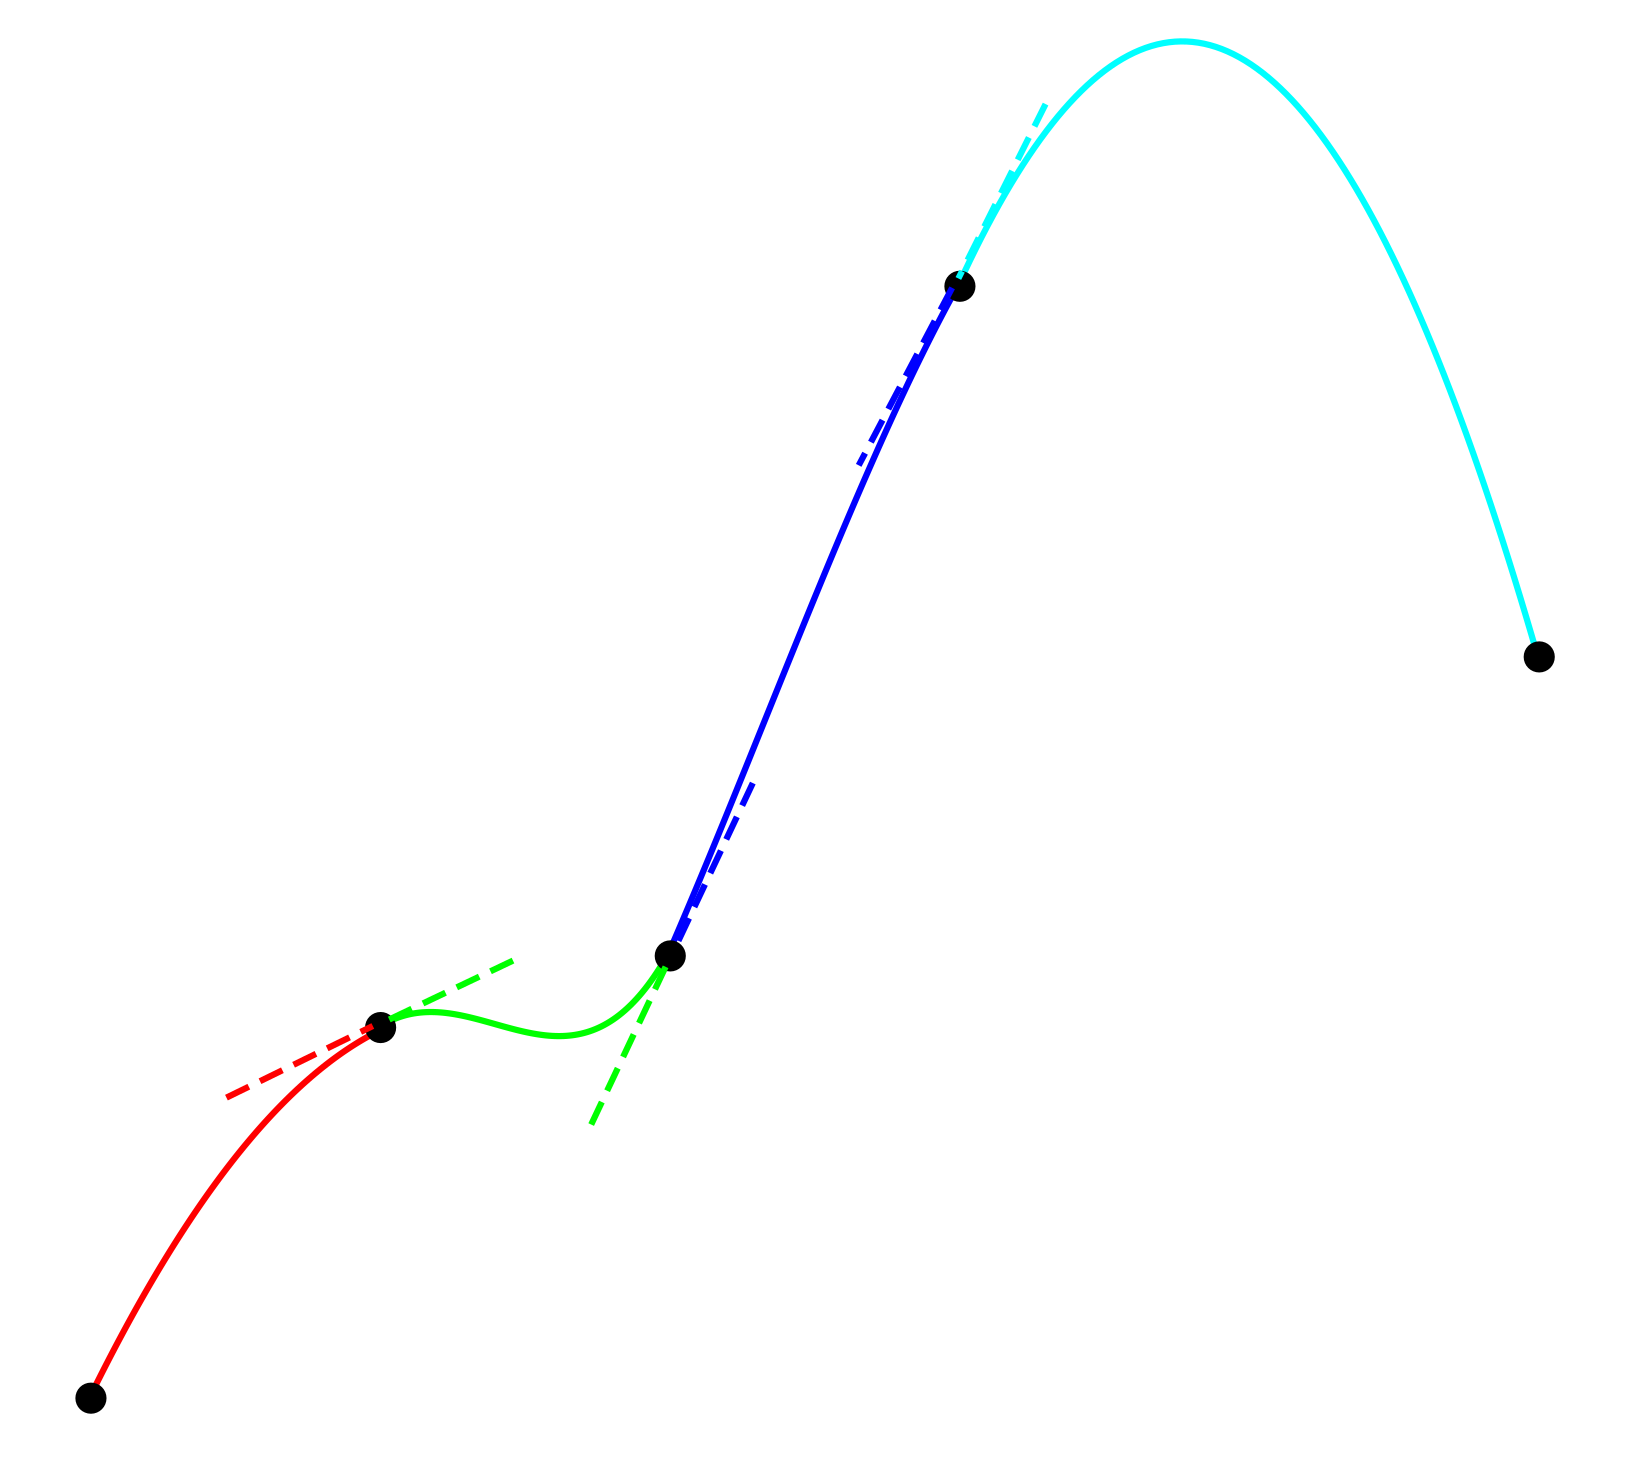
\includegraphics{new-spline.png}
	\end{center}
	\caption{Схематическое изображение аппроксимации сплайном, сплошная линии разных цветов --- полиномы составляющие сплайн, пунктирной линией показана касательная на границах }\label{fig:old.regress.spline}
\end{figure}

Для аппроксимация кубическим и параболическим сплайном в Mathcad есть встроенные функции \mc{cspline(x,y)} и \mc{pspline(x,y)} соответственно. Аргументами являются векторы исходных данных $x$ и $y$. В результате функция возвращает вектор, содержащий параметры полиномов в каждом из диапазонов. Для вычисления значения сплайн функции точке \mc{xt}, необходимо воспользоваться функцией \mc{interp(vs,x,y,xt)}.




\primer{Задайте произвольный набор данных \mc{x} и \mc{y} в виде таблицы. Для аппроксимации данных используете кубический сплайн и полином третьей степени. Постройте графики полученных функций и сравните результат.}
%пример решения
\begin{center}
	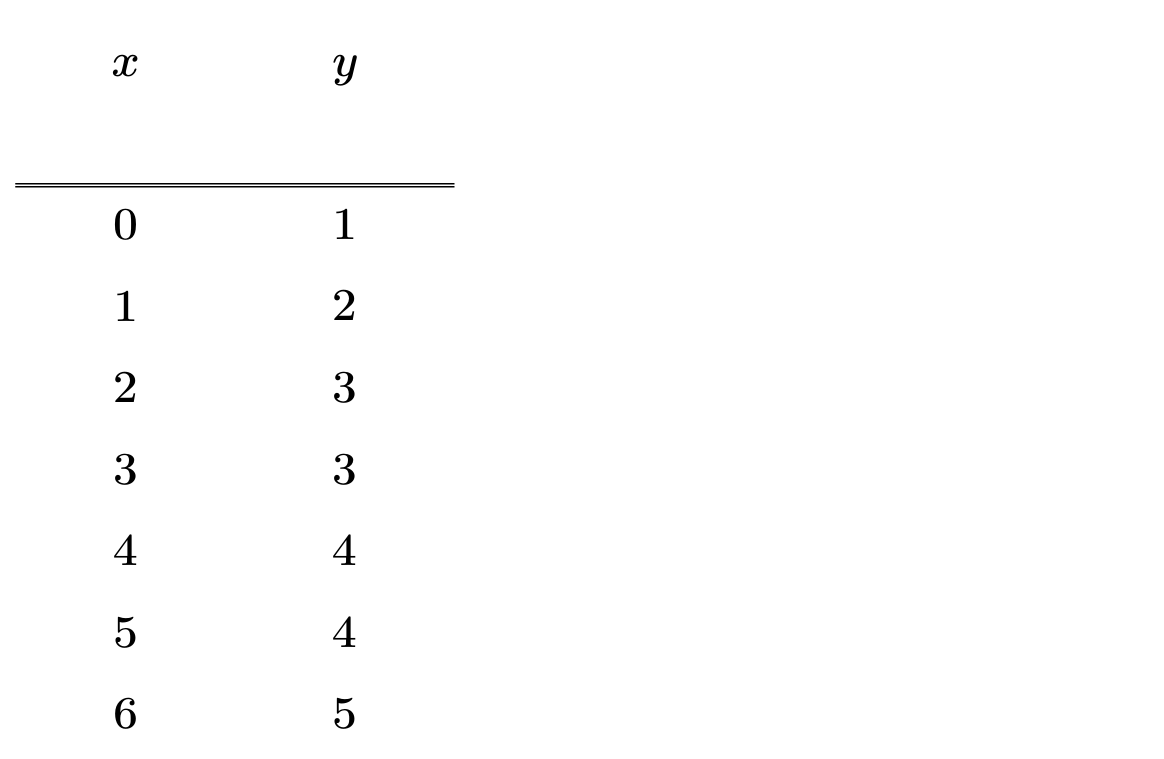
\includegraphics{new-regress-5-1.png}
\end{center}

\begin{center}
	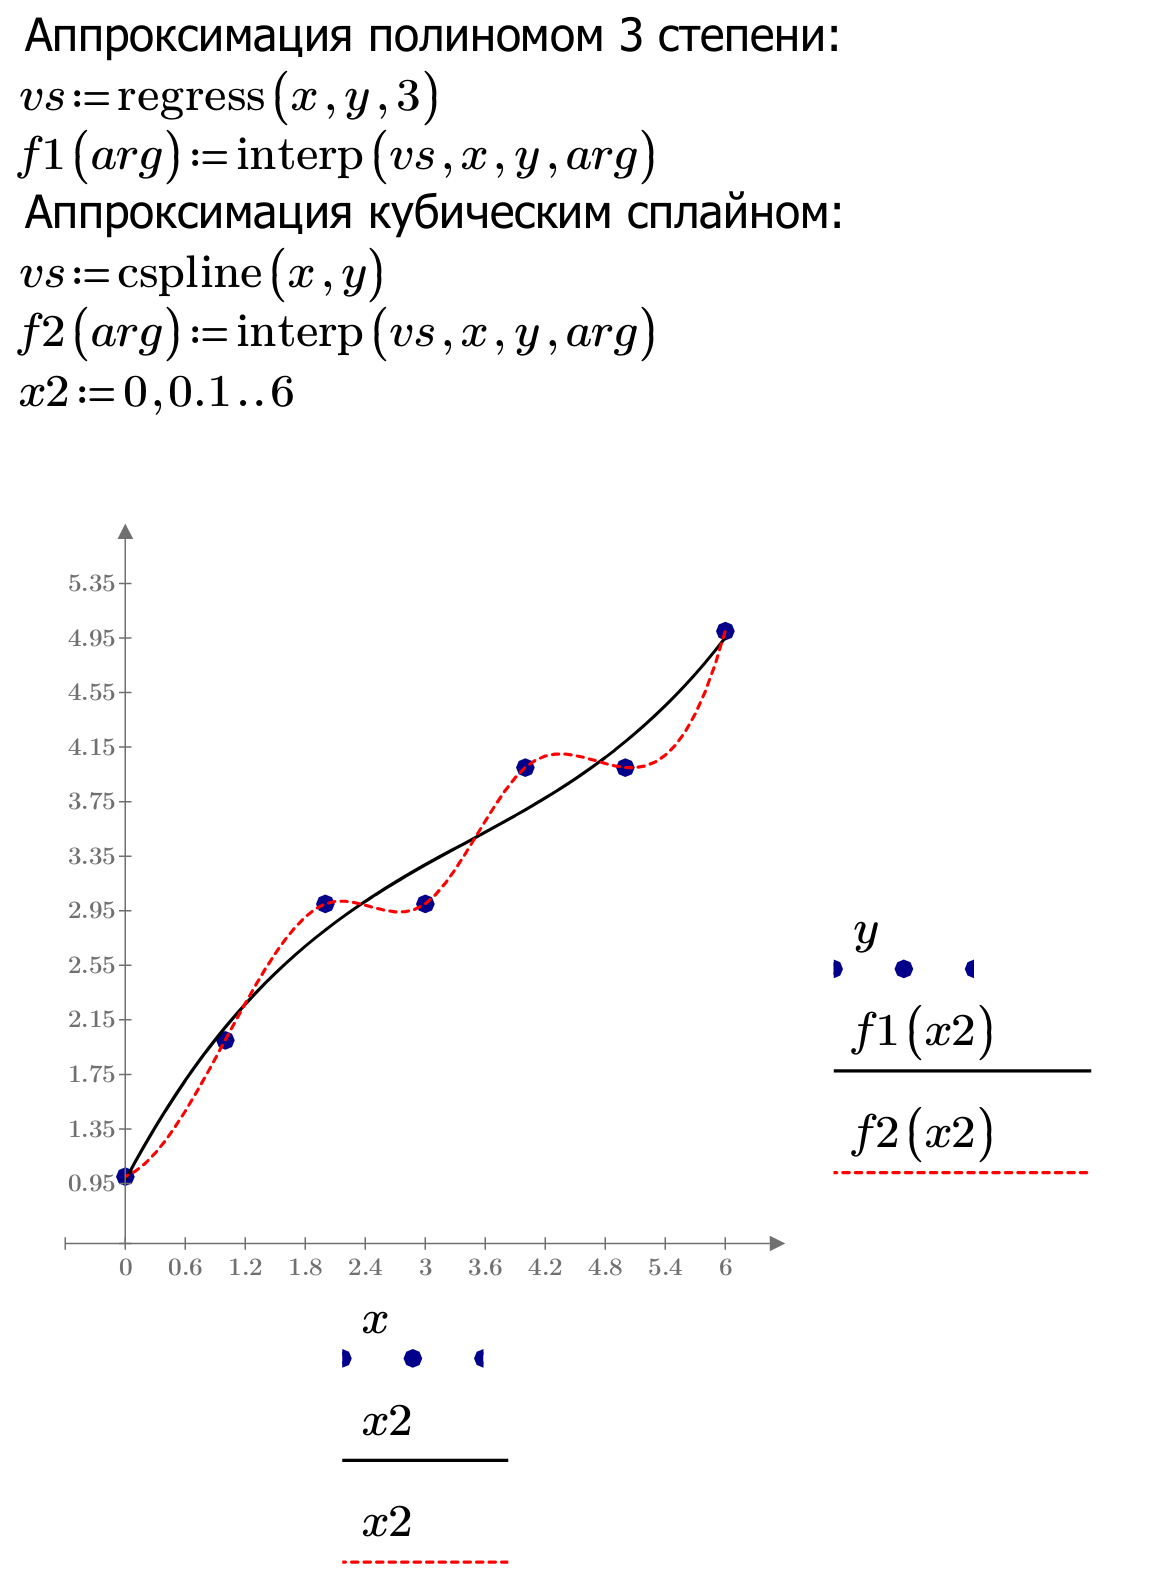
\includegraphics{new-regress-5-2.png}
\end{center}

Вопросы для самоконтроля:
\begin{enumerate}
	\item Что такое регрессионный анализ?
	\item Что такое коэффициент корреляции?
	\item Какие виды функций регрессии существуют, в чем их различие?
	\item Какие функции решения уравнения с одним неизвестным и системы уравнений используются в MathCad?
\end{enumerate}

\subsubsection*{Пример задания}
\begin{enumerate}
\item В результате измерения зависимости переменной состояния $y$ от входного фактора $x$ были получены значения, представленные в таблице. Описать табличные данные следующими функциональными зависимостями:
\begin{itemize} 
	\item $y(x)=a x+b$
	\item $y(x)=a_3 x^3 +a_2 x^2 + a_1 x +a_0$
	\item $y(x)=a e^{b x}+c  $
	\item $y(x)=a \cdot x^b+c$
	\item $y(x)=a_0 x                     +a_1 x^{3.7}                +a_2 \sqrt{x}              $
	\item $y(x)=A \cdot e^{-\dfrac{B}{x}+C}        $
	\item параболический сплайн
\end{itemize}
\begin{table}[h]
	\begin{tabular}{|c|c|}
		\hline
		x & y \\ \hline
		7.80 &     -62.58 \\ \hline 
		9.10 &    -116.08 \\ \hline 
		10.40 &    -157.64 \\ \hline 
		11.70 &    -143.06 \\ \hline 
		13.00 &    -257.91 \\ \hline 
		14.30 &    -386.64 \\ \hline 
		15.60 &    -323.30 \\ \hline 
	\end{tabular}
\end{table}

\item  Используя данные из справочника теплофизических свойств \cite{vargaftik} описать удельный объем изобутана при р = 1 атм изобутана. В качестве аппроксимирующей функции может выступать любое выражение, однако максимальное отклонение не должно превышать 10\%. Определить, при какой температуре удельный объем изобутана при р = 1 атм равен $   657.0 \frac {\text{дм}^3}{\text{кг}}$.
\end{enumerate}
		\laborator{Решение дифференциальных уравнений}

\goal ознакомиться с возможностями математического пакета Mathcad при решении дифференциальных уравнений в различных вариантах постановки задачи (задача Коши, краевая задача).

\subsubsection*{Теория}

Дифференциальные уравнения позволяют выразить соотношения между изменениями физических величин, и потому они имеют большое значение в прикладных задачах. Обыкновенным дифференциальным уравнением порядка $r$ называется уравнение:
\begin{equation} \label{dif.mdif}
	F(x,y(x),y^\prime(x),y^{\prime \prime}(x), ... , y^r(x))=0,
\end{equation}
которое связывает независимую переменную $x$, искомую функцию и ее производные. Решение (интегрирование) дифференциального уравнения \ref{dif.mdif} заключается в отыскании функций (интегралов), которые удовлетворяют этому уравнению для всех значений  в определенном конечном  или бесконечном интервале. Решения могут быть проверены подстановкой в уравнение \ref{dif.mdif}.

Общее решение обыкновенного дифференциального уравнения порядка $r$ имеет вид:
\begin{equation}
	y=y(x,C_1,C_2, ... ,C_r),
\end{equation}
где $С_1$, $С_2$, ... , $С_r$ --- произвольные постоянные (постоянные интегрирования). Каждый частный выбор этих постоянных дает частное решение. В задаче Коши (начальной задаче) требуется найти частное решение, удовлетворяющее $r$ начальным условиям:
\begin{equation}
	y(x_0)=y_0, \newline
	y^{\prime}(x_0)=y_0^{\prime}, ... , y^{r}(x_0)=y^r_0,
\end{equation}
по которым определяются $r$ постоянных $С_1$, $С_2$, ... , $С_r$. В краевой задаче на $y(x)$ и ее производные накладываются $r$ краевых условий в точках $x=a$ и $x=b$.

Методы численного решения обыкновенных дифференциальных уравнений в форме задачи Коши разработаны досконально \cite{shipachevvs2005}. Самыми распространенными из них являются алгоритмы Рунге~-- Кутта, успешно используемые для решения подавляющего большинства дифференциальных уравнений. 

В Mathcad имеются специальные встроенные функции, позволяющие находить решения как линейных, так и нелинейных систем дифференциальных уравнений. Несмотря на различные методы поиска решения, каждая из этих функций требует, чтобы были заданы, по крайней мере, следующие величины, необходимые для поиска решения:
\begin{itemize}
	\item начальные условия; 
	\item набор точек, в которых нужно найти решение;
	\item само дифференциальное уравнение, записанное в некотором специальном виде.
\end{itemize}
Для качественного и быстрого решения подавляющего большинства систем дифференциальных уравнений используется функция \mc{ rkfixed(у0, t0, t1, М, D)}. Данная функция решает задачу Коши с помощью алгоритма на основе метода Рунге~-- Кутта 4-го порядка с фиксированным шагом.
При использовании функции \mc{rkfixed} для решения системы дифференциальных уравнении первого порядка:
\begin{equation}\label{dif.tosol1}
	y_i^{\prime}(x)=F(x,y_i(x)),\quad i=1, ... ,N
\end{equation}
она должна быть записана в векторном виде:
\begin{equation}\label{dif.tosol2}
	y(x)=D(y(x),x),
\end{equation}
где $y(x)$ --- вектор первых производных системы; $D(y(x),x)$ --- вектор~-- функция, каждая строка которой содержит правую часть соответствующего уравнения системы \ref{dif.tosol1}.

Параметры функции \mc{rkfixed} определяются следующим образом:
 \begin{itemize}[label={}]
 	\item \mc{y0} --- вектор значений искомых функций на левой границе интервала изменения переменной. Размерность вектора определяется порядком дифференциального уравнения или числом уравнений в системе (если решается система уравнений). Для дифференциального уравнения первого порядка вектор начальных значений вырождается в одну точку $y_0 = y(x_0)$;
 	\item \mc{t0} и \mc{t1} – начальная и конечная точки интервала, на котором ищется решение системы дифференциальных уравнений;
 	\item \mc{М} --- число точек, за исключением начальной точки, в которых будет определяться решение системы дифференциальных уравнений. Длина шага вычисляется делением интервала \mc{t1 - t0}, на число шагов \mc{М}. Величина mc{M} влияет на точность и трудоемкость численного решения системы дифференциальных уравнений. Большой шаг снижает точность и трудоемкость решения, маленький шаг, наоборот, повышает точность, но одновременно и трудоемкость. Данный факт необходимо учитывать при выборе значения \mc{М}. Число \mc{М} определяет число строк в полученной матрице решений, которое равно \mc{М+1};
 	\item \mc{D(x,y)} --- вектор-функция, содержащая правые части уравнений системы \ref{dif.tosol1}. Должна быть задана как функция двух переменных: скаляра \mc{х} (аргумента функции) и вектора \mc{у} (все искомые функции системы должны быть представлены как элементы одного вектора \mc{у}).
 \end{itemize}
 
Результатом работы функции \mc{rkfixed} является матрица, в первом столбце которой содержатся значения переменной \mc{t} (от \mc{t0} до \mc{t1}), а в остальных --- значения неизвестных функций системы, рассчитанные в заданных точках. При этом порядок расположения столбцов искомых функций определяется последовательностью, в которой они были занесены в вектор \mc{у}.

\primer{Решить дифференциальное уравнение $\frac{dy}{dx}+3y =0$	начальным условием $у(0) = 4$. Интервал решения [0,4]. Результат решения представить графически.}

\begin{center}
	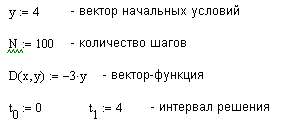
\includegraphics{olddiff-z1-1.png}
\end{center}

\begin{center}
	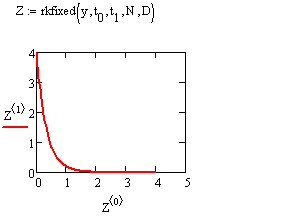
\includegraphics{olddiff-z1-2.png}
\end{center}

\primer{Решить систему дифференциальных уравнений в интервале [-2; 8] с начальными условиями $y(-2)=1$ и $z(-2)=-10$
\begin{equation*}
	\begin{cases}
		\dfrac{d y(x)}{d x} - (y(x)-z(x)) \sin(x)=0 \\
		\dfrac{d z(x)}{d x} -\sqrt[3]{y(x)} +z(x) = 0
	\end{cases}
\end{equation*}
Результат решения представить графически. }

\begin{center}
	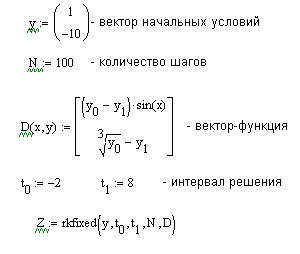
\includegraphics{olddiff-z2-1.png}
\end{center}

\begin{center}
	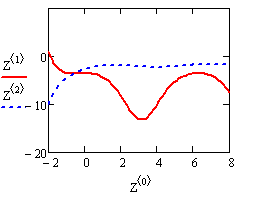
\includegraphics{olddiff-z2-2.png}
\end{center}

\subsubsection{Дифференциальные уравнения высших порядков}
Если дифференциальные уравнения системы содержат производные от неизвестных функций выше первого порядка, то все уравнения, содержащие такие производные, необходимо преобразовать. Любое уравнение вида \ref{dif.mdif}, содержащее производные выше первого порядка посредством замены:
\begin{equation}
	\begin{gathered}
		y_1(x)=y(x),\\ y_2(x)=y^{\prime}(x),\\  ... \\ y_r(x)=y^r(x)
	\end{gathered}
\end{equation}
может быть приведено к совокупности уравнений:
\begin{equation}
	\begin{gathered}
		y_1^{\prime}(x)=y_2(x), \\ y_2^{\prime}(x)=y_3(x), \\ ... \\ y_r^{\prime}(x)=F(x,y_1(x),y_2(x, ... , y_r(x))
	\end{gathered}
\end{equation}
В приведенных выше уравнениях уже нет производных выше первого порядка. Преобразовав подобным образом каждое из уравнений, входящих в исходную систему, получим новую систему с большим количеством неизвестных функций, но с производными только первого порядка. Следовательно, для решения такой системы дифференциальных уравнений можно использовать функцию \mc{rkfixed}, как описано выше.

\primer{Решить систему дифференциальное уравнений второго порядка $y^{''}+y^{'}-y-x=0$. Построить график функции $y$.}
\begin{center}
	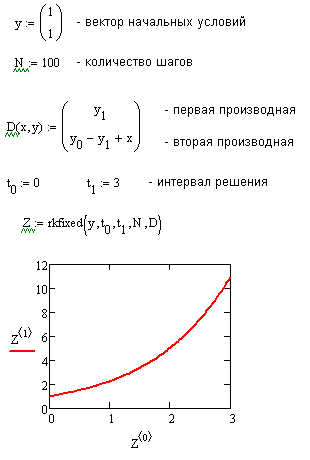
\includegraphics{olddiff-z3.png}
\end{center}


\subsubsection*{Решение краевых задач}

Краевые задачи отличаются от задач Коши тем, что начальные условия для них задаются на обеих границах интервала поиска решений. Краевая форма для дифференциальных уравнений и их систем используется в основном в физике и технике в тех случаях, когда определить все начальные значения на одной границе интервала невозможно. 

Найти решение для заданных таким образом дифференциальных уравнений возможно только на основе алгоритма, в котором многократно решается задача Коши. Суть этого алгоритма заключается в подборе (естественно, направленном) недостающих параметров на одной из границ интервала, исходя из того условия, что соответствующие решения полученной задачи Коши в противоположной точке интервала должны совпадать с исходными краевыми условиями с определенным уровнем точности.

Для решения краевых задач в Mathcad имеется встроенная функция \mc{sbval(z,t0,t1,D,load,score)}. Данная функция требует определения следующих параметров:
\begin{itemize}[label={}]
	\item \mc{z} --- вектор приближений, в котором необходимо определить исходные значения для недостающих на левой границе условий. Выбор начального приближения оказывает влияние на сходимость и время поиска решения;
	\item \mc{t0} и \mc{t1} --- начальная и конечная точки интервала, на котором ищется решение системы дифференциальных уравнений;
	\item \mc{D(x,y)} --- вектор-функция, описывающая дифференциальное уравнение или систему уравнений. Задается аналогично рассмотренной ранее встроенной функции \mc{rk\-fix\-ed};
	\item \mc{load(t0,z)} --- векторная функция двух переменных, описывающая значение функции на левой границе интервала. Представляет собой вектор из \mc{N} элементов (\mc{N} соответствует количеству уравнений системы), каждый из которых является значением соответствующей функции вектора \mc{y} в точке \mc{t0}. Если начальное значение некоторой функции неизвестно, в качестве элемента \mc{load} следует использовать величину из вектора приближений \mc{z};
	\mc{score(t1,y)} --- векторная функция, служащая для задания правых граничных значений. Элементы вектора \mc{score} должны быть заданы как разности известных начальных значений в точке \mc{t1} и соответствующих им значений функций \mc{y}, возвращаемых функцией \mc{sbval}. Алгоритм, лежащий в основе функции \mc{sbval}, использует текущие величины \mc{score} в качестве меры точности подобранных приближений. 
\end{itemize}

Результатом работы функции \mc{sbval} является вектор с найденными значениями начальных условий, недостающих для представления системы дифференциальных уравнений в форме задачи Коши. Определив начальные условия, можно решить данную систему дифференциальных уравнений используя встроенную функцию \mc{rkfixed}.  При этом  в качестве  ее параметра \mc{у0} можно использовать уже определенную выше функцию \mc{load} (обозначив вектор результата как \mc{z}).

\primer{Решить краевую задачу для систем дифференциальных уравнений в интервале [0; 2] с граничными условаиями $y(0)=3$ $z(2)=1.598$:
\begin{equation*}
	\begin{cases}
		\dfrac{d y(x)}{d x} + 3 x y(x) -z(x) =0 \\
		\sqrt[3]{z(x)} -y(x) - \dfrac{d z(x)}{d x}  = 0
	\end{cases}
\end{equation*}
Результат решения построить графически.
}
\begin{center}
	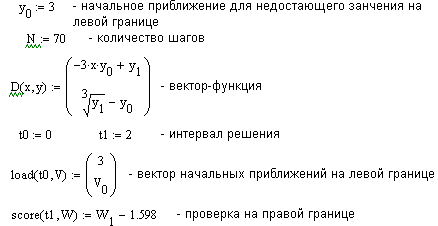
\includegraphics{olddiff-z4-1.png}
\end{center}

\begin{center}
	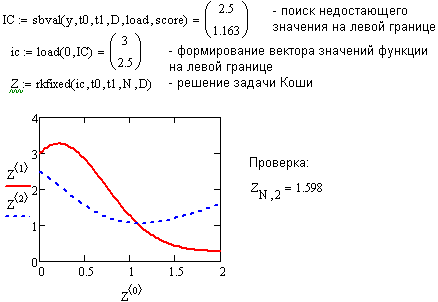
\includegraphics{olddiff-z4-2.png}
\end{center}

\subsubsection*{Примеры составления дифференциальных уравнений}
\primer{ В сосуд объемом $V\ м^3$ содержащий чистую воду, подведено две трубы. По трубам поступает $j_1$ и $j_2 \frac{м^3}{ч}$ раствора соли, концентрацией $c_1$ и $c_2$ соответственно. Раствор мгновенное перемешивается, что соответствует модели идеального смешения. Излишки смеси вытекают в канализацию. Необходимо составить математическую модель для описания массы соли находящейся в сосуде.}

При составлении дифференциального уравнения необходимо учитывать входящие и выходящие потоки массы. Входящие потоки увеличивают массу соли в сосуде, и записываются в дифференциальное уравнение со знаком +, выходящие --- соответственно со знаком $-$. Масса соли, приходящая с первым потоком равна $j_1 c_1$, со вторым --- $j_2 c_2$. Выходящий поток имеет ту же концентрацию, что и в самом сосуде и может быть выражена через массу соли в сосуде и его объем $c=\frac{m}{V}$.

Соответственно уравнение изменения массы по времени будет записано в виде:
\begin{equation}
	\dfrac{d m}{d \tau} = j_1 c_1 + j_2 c_2 - (j_1 + j_2 ) \dfrac{m}{V}
\end{equation}

Дифференциальное уравнение дополняем начальными условиями: в начальный момент времени в сосуде содержится чистая вода, соответственно $m(0)=0.$

\primer{В баке цилиндрической формы (высота $h$ 1 м, диаметр $D$ 30 см) проделали круглое отверстие диаметром 0.5 см. Бак доверху наполнили водой закрыв отверстие. Определить, через какое время в баке останется 15 литров воды? }

Усредненная по поверхности отверстия скорость истечения равна:
\begin{equation}
	\bar{w}=\phi \sqrt{2gH}
\end{equation} 
где $\phi$ --- коэффициент скорости, для отверстий в тонкой стенке равный 0.97, $H$ --- высота столба жидкости в резервуаре надо отверстием.

Расход жидкости можно записать умножая скорость истечения на площадь отверстия:
\begin{equation}
	\dfrac{d V}{d \tau} = - S \varepsilon \bar{w}= -S \varepsilon  \phi \sqrt{2gH}
\end{equation}
где $\varepsilon$ --- коэффициент сжатия струи, для отверстий в тонкой стенке равный 0.64. Знак  <<->> в дифференциальном уравнении показывает,  что в объем воды в резервуаре течением времени уменьшается. 

Дифференциальное уравнение дополняем начальным условием: в начальный момент времени резервуар полный, следовательно $V(0)=\frac{h D^2}{4}$


\primer{В комнату объемом 10 $\mathrm{м^3}$ и температурой воздуха 20 $\mathrm{C^\circ}$ внесли разогретый до 100 $\mathrm{C^\circ}$ предмет массой 5 кг, теплоемкость материала 10 ${\frac{Дж} {кг С^\circ}}$. Считая комнату плотностью изолированной, и принимая условие высокой теплопроводности как тела, так и воздуха, определить температуру воздуха через 1 час при условии что коэффициент теплоотдачи равен 120 ${\frac{Вт}{м^2 К}}$  }
 
Уравнение теплопередачи имеет вид:
\begin{equation}
	q=K F \Delta T
\end{equation}
где $q$ --- тепловой поток, $F$ --- поверхность теплопередачи, $\Delta T$ --- разница температур двух тел. Изменение температуры тела можно определить по количеству тепла, принятого или отданного телом:
\begin{equation}
	\dfrac{d T}{d \tau}=\dfrac{q}{c m} = \dfrac{K F \Delta T}{c m}
\end{equation}
где $c$ --- теплоемкость тела, $m$ --- масса тела.
теперь можно записать систему уравнений:
\begin{equation}
	\begin{cases}
	\dfrac{d T_1}{d \tau} = \dfrac{-K F (T_1-T_2)}{c_1 m_1} \\
	\dfrac{d T_2}{d \tau} = \dfrac{K F (T_1-T_2)}{c_2 m_2}
	\end{cases}
\end{equation}
индексами 1 и 2 обозначены соответственно разогретый предмет и окружающий воздух. В первом уравнении знак <<->> означает, что тело отдает тепло, соответственно температура тела уменьшается.

\primer{Толщина стенки теплоизоляции $l=3 см$, теплопроводность стенки $\lambda=0.4 \dfrac{Вт} {м \cdot гр}$. Температура горячей стороны теплоизоляции $T_г=120 \mathrm{C^\circ}$. Определить температуру с холодной стороны, если тепловой поток равен $50 \frac{Вт}{м^2}$}

Распределение температуры вдоль стенки теплоизоляции можно определить по закону Фурье:
\begin{equation}
	q=-\lambda \dfrac{d T}{d x}
\end{equation} 
В случае постоянства теплового потока $q$ и теплопроводности $\lambda$ можно записать дифференциальное уравнение:
\begin{equation}
	\dfrac{d T}{d x} =- \dfrac{q}{\lambda}
\end{equation}
Аналитическое решение уравнения дает:
\begin{equation}
	 T = T_г - \dfrac{q x}{\lambda}
\end{equation}

Вопросы для самоконтроля:
\begin{enumerate}
	\item Что такое обыкновенное дифференциальное уравнение и чем определяется его порядок?
	\item Какие данные необходимы для поиска решения дифференциального уравнения?
	\item Что является решением дифференциального уравнения?
	\item Что такое задача Коши?
	\item Что такое краевая задача?
	\item Что влияет на точность и трудоемкость численного решения системы дифференциальных уравнений?
\end{enumerate}

		\laborator{Основы программирования в пакете Mathcad}

\goal ознакомиться с возможностями языка программирования математического пакета Mathcad; рассмотреть основные операторы и приемы программирования в Mathcad.

Теория
Язык программирования Mathcad содержит все элементы языка высокого уровня, необходимые для математических расчетов. Кроме того, он содержит дополнительно сотни встроенных функций и операторов системы Mathcad, имеет возможности численного и символьного расчета различных величин, и поэтому по эффективности не уступает профессиональным системам программирования.
Все операторы и элементы языка программирования Mathcad расположены на рабочей панели «Программирование». Даная панель содержит восемь пиктограмм, соответствующих операторам языка программирования Mathcad. 
Чтобы написать программу, прежде всего для нее должен быть создан специальный обособленный от остального документа блок. Выглядит он как черная вертикальная линия с маркерами, в которые заносятся те или иные выражения алгоритма. Чтобы построить единичный элемент программного блока, нажмите пиктограмму «Добавить строку программы» панели «Программирование» (клавишей «]»). При этом в области курсора появится следующий объект:

Обычно программа содержит больше чем две строки, поэтому лучше сразу задать блок из 5-6 маркеров. Сделать это можно, последовательно нажав нужное количество раз соответствующую кнопку панели «Программирование» или «]». 
Чтобы добавить строку к уже созданному блоку, поставьте курсор в ту строку блока, выше или ниже которой должна быть введена строка. Положение вставляемого маркера определяется положением синей вертикальной черты курсора. Если она находится слева от выделенного выражения, то маркер будет добавлен выше выделенной строки, если справа – то ниже. Чтобы развернуть курсор в нужную сторону, нажмите клавишу «Insert».
Программный блок можно создать и внутри уже заданного блока. Для этого используйте один из стандартных способов, поставив курсор в маркер любого из операторов программирования:

Созданный таким образом блок выглядит как параллельная главному блоку линия. Выражения, внесенные в него, будут обособлены от остальной программы, и выполнение соответствующих действий будет связано только с оператором, к которому относится внутренний блок.
Для присвоения значений переменным и функциям в программах Mathcad используется специальный оператор: «» – «Локальное определение» (панель «Программирование») или сочетание Shift+«[». Использовать оператор обычного присваивания «:=» в программах нельзя.
Присваивание значений в программах имеет ряд особенностей. Присвоение величин используемым алгоритмом функциям и переменным может быть произведено как в самой программе, так и выше нее. Если значение переменной или функции присваивается в программе посредством оператора «», то такая переменная или функция будет являться локальной, то есть она будет видимой только в рамках программы. Как-то повлиять на объекты вне программы она не сможет (равно как извне к ней нельзя будет получить доступ). Если переменная или функция задаются выше программы с помощью оператора «:=», то она будет обладать глобальной видимостью, то есть такая переменная или функция будет доступна любому нижележащему объекту, в том числе и коду программ. Однако программа может только прочитать значение глобальной переменной или вызвать глобальную функцию. Как-то изменить значение глобальной переменной или функции программа не может. Если программа должна осуществлять какую-то модификацию объекта (например, возводить все элементы массива в квадрат), то результат своей работы она должна возвращать.
Локальные переменные и функции имеют приоритет над глобальными в рамках «родной» программы. Это означает, что если имеется локальная и глобальная переменные (или функции) с одним именем, то обращение по этому имени будет адресоваться к локальной переменной (или функции).
3адание 1

1.1.Задайте переменную А, далее создайте программный блок, где этой же переменной присвойте новое значение и выведите его на печать. После выполнения блока распечатайте значение переменной.



1.2. Значение переменной, полученной в результате выполнения программы (1.1.), присвойте новой переменной, что бы она была доступна вне программы. 



Как видно из задания, в результате выполнения программы значение переменной А изменено не было.
Mathcad позволяет в теле программы задать локальную пользовательскую функцию. Создаются локальные функции точно так же, как обычные (только в качестве оператора присваивания используется ). Вызвать локальную функцию можно только из нижележащих строк программы. Вне программы она не доступна.

3адание 2

Задайте пользовательскую функцию $f(x,y,z) = sin(x)+sin(y)+sin(z)$. Обратитесь в теле программы к данной функции несколько раз и распечатайте полученное значение.



Если необходимо ввести большое число локальных переменных, то это можно сделать, используя следующие приемы:
1. С помощью матрицы строки. В маркере программного блока создается матрица-строка из n элементов, после этого определяется каждая переменная в маркерах данной матрицы.



2. Проведение присваивания в строке через запятую. Для этого поставьте курсор в маркер программного блока и последовательным нажатием клавиши «,» введите необходимое количество маркеров, после чего в каждом из них задайте переменную либо пропишите требуемое действие.



Данные приемы позволяют сократить длину программы.
Построение программ проводится с использованием специальных управляющих операторов, вроде оператора цикла for или оператора условия if. Чтобы задать нужный оператор, используйте соответствующие кнопки панели «Программирование». Просто набрать оператор с клавиатуры нельзя – он будет воспринят системой Mathcad как неизвестная функция.
Такие операторы, как if, for, while, активируют код, помещенный в их левый маркер, в том случае, если выполняется условие в правом. Для задания условия используются такие операторы панели «Булева алгебра», как . Можно задать и комплекс условий, задействовав оператор логического И  панели «Булева алгебра», или оператор логического ИЛИ .

Операторы цикла (for, while)
Оператор простого цикла for позволяет организовать выполнение операции или проверку условия для ряда конкретных значений переменной. Оператор for задается с помощью команды панели «Программирование» или сочетанием клавиш (Ctrt+Shift+«'»). Оператор for имеет три маркера:



В двух верхних маркерах, соединенных символом принадлежности, задается имя переменной, по которой организуется цикл, и ряд принимаемых ею значений. В нижнем маркере определяется операция или комплекс операций, которые должны быть выполнены для каждого значения переменной. Ряд значений переменной обычно представляет собой последовательность целых чисел, которая задается с помощью ранжированной переменной. Для этого в правый верхний маркер вводится оператор ранжированной переменной (панель «Матрица»), по умолчанию ряд будет содержать целые значения с шагом 1. Если значения переменной должны изменяться с меньшим или большим шагом, то это можно сделать, введя в правом маркере оператора ранжированной переменной через запятую первое и второе значения в ряде переменной (разница между ними и задаст шаг).



Если операция или комплекс операций должны быть просчитаны при ряде некоторых конкретных значений переменной, причем ряд этот нельзя задать математически в общем виде, его можно непосредственно определить в правом верхнем маркере оператора for в виде вектора:



С помощью второго оператора цикла while (Пока) (сочетание клавиш Ctrl-«]») можно организовать цикл, который будет работать до тех пор, пока выполняется некоторое условие. Оператор while имеет два маркера, в которые вводятся соответственно условие работы цикла и выражения операций, которые должны быть проделаны на каждом его витке:



В цикле while количество его витков не нужно определять явно. Итерации будут совершаться до тех пор, пока будет выполняться условие в правом маркере.



Если возникает необходимость прервать работу цикла, то можно использовать оператор break (Прервать). Ввиду того, что цикл бывает нужно остановить при выполнении некоторого условия, оператор break почти всегда используется с условным оператором if.

Задание 3

Используя операторы цикла, замените значения элементов произвольного массива A размерностью 3х3 их квадратами. Полученные значения присвойте новой переменной.



Условные операторы (if, otherwise)
Условный оператор if имеет два маркера:



В правый маркер вводится условие, в левый – операция, которая должна быть проделана в случае, если условие выполнится (если же оно не выполняется, система просчитывает программу, пропуская данный фрагмент). Как уже говорилось, в маркер оператора может быть внесено несколько условий. 
Оператор otherwise (Иначе) предназначен для определения того действия, которое должно быть выполнено, если условие оператора if (Если) окажется неистинным. 
Если по условию необходимо выполнить не одну, а несколько операций, то в этом случае курсор помещается в левый маркер и нажатием пиктограммы «Добавить строку программы» или клавиши «]» добавляется необходимое количество строк.


В этом случае операции, которые необходимо выполнить, записываются в блок после оператора if (или otherwise).

Задание 4

Используя условные операторы, создайте блок программы для определения переменных А и B, которые будут принимать значения в зависимости от переменной N. Если N>0, то . Результат представить в двух вариантах: результат распечатать; результат присвоить переменой С.



Вопросы для самоконтроля:
1. В какой пиктограмме содержатся операторы и элементы языка программирования Mathcad?
2. Чем визуально отличается блок программы от остального документа?
3. Какой оператор используется для присвоения значений переменным в программных блоках?
4. Какие операторы цикла есть в пакете Mathcad? В чем их отличие?
5. Какие условные операторы цикла есть в пакете Mathcad?

		}
	{new}{now this is b}
	{octave}{\laborator{Основы математического пакета GNU Octave}

GNU Octave является высокоуровневым языком программирования, ориентированным на численное решение математических задач. Данный пакет разрабатывался как свободная альтернатива популярному пакету Matlab. В связи с этим синтаксис программ этих двух языках идентичен. Несмотря на меньшее количество подключаемых библиотек, более низкую производительность (отчасти за счет отсутствия поддержки многопотоковых вычислений) пакет Ocatve обладает всем необходимым функционалом как для академического, так и для использования на практике при инженерных расчетах.
На момент написания методического указания, Octave и подключаемый набор библиотек активно развиваются.

\section*{Установка}
Пакет Octave распространяется под лицензией GNU, позволяющих модификацию исходного кода, что позволяет скомпилировать его под множество операционных систем. Для большинства популярных Linux дистрибутивов пакет Octave уже включен в стандартные репозитории. Существуют сборки для Windows, MacOS, BSD (https://www.gnu.org/software/octave/download.html). Также существует портированная на android версия  

\section*{Графическое приложение}



\section*{Переменные}

\section*{Массивы}

\section*{Функции}

\section*{Программирование}

\section*{Работа с файлами}

\section*{Графики}

}}


%

%octave
\laborator{Определение условий фазовых равновесий пар~-- жидкость}

\goal на основе экспериментальных данных по давлению насыщенных паров чистых компонентов определить условия фазовых равновесий пар~-- жидкость бинарной идеальной смеси при различных термодинамических условиях; результаты представить в виде диаграмм фазового равновесия ($у-х$; $Р-х, у$; $Т-х, у$).

\subsubsection{Теория}

Химической промышленности в основном приходится иметь дело с системами, представляющими собой смеси газов и жидкостей, которые необходимо разделять. При проектировании процессов разделения подобных систем необходимо иметь данные о равновесных свойствах смесей. Условия фазового равновесия удобно представлять в виде фазовой диаграммы, которая описывает влияние температуры, давления и состава на вид и число фаз, которые могут сосуществовать при данных условиях. Число фаз определяется согласно правилу фаз Гиббса. Вид фаз, которые могут сосуществовать в конкретных условиях, зависит от химической природы компонентов. Представление фазового равновесия более удобно в графическом виде, чем в табличном, так как позволяет охватить взаимные связи между переменными.

В соответствии с правилом фаз Гиббса для любой термодинамически равновесной системы число параметров состояния $С$ (степеней свободы), которые можно изменять, сохраняя число существующих фаз $Ф$ неизмененным, определяется выражением
\begin{equation}
С=К-Ф+N,
\end{equation}
где $К$ – число компонентов системы, $N$ – число параметров состояния системы, имеющих одно и то же значение во всех фазах (обычно температура $Т$ и давление $p$, $N$ = 2). Величина $С$ определяет число параметров состояния, которые нужно задать для однозначного определения состояния системы.

Из правила фаз следует, что в однокомпонентной системе ($К$ = 1) в однофазной области ($Ф$ = 1) состояние системы определяется двумя параметрами ($С$ = 2) $Т$ и $p$ (можно произвольно и одновременно изменять оба параметра до тех пор, пока система не окажется на одной из ограничивающих область линий). На линиях фазового равновесия ($Ф$ = 2) состояние системы определяется одним параметром ($С$ = 1) (произвольно можно менять только один из параметров – $p$ или $Т$ (если изменяется $Т$, то $p$ будет изменяться в соответствии с ходом кривой, и наоборот)). В трехфазной области ($Ф$ = 3) число степеней свободы равно нулю ($С$ = 0), что соответствует тройной точке (в этой точке ни один из параметров не может быть изменен, равновесное сосуществование трех фаз однокомпонентной системы возможно только при строго определенных значениях $Т$ и $p$.). Для любой системы число фаз максимально, когда $С$ = 0. При увеличении числа компонентов $К$ в системе растет число параметров состояния $С$, необходимых для однозначного определения состояния системы.

Как было показано выше, для однокомпонентной системы максимальное число степеней свободы равно двум, соответственно фазовое равновесие такой системы можно представить на плоскости в виде двухкоординатной фазовой диаграммы (\cref{fig:phase-id.f1}). Для двухкомпонентной системы число степеней свободы равно трем. Взаимозависимость трех переменных можно отразить лишь посредством пространственных диаграмм. На практике работать с трехмерными диаграммами уже сложнее, чем с двухмерными. Для трехкомпонентной системы число степеней свободы равно четырем и представить фазовую диаграмму такой системы графически уже затруднительно.

\begin{figure}
	\begin{center}
		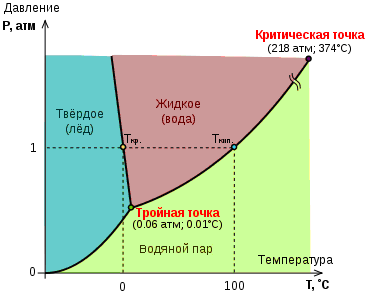
\includegraphics[width=0.7\textwidth]{phase-id-f1.png}
	\end{center}
	\caption{Двухкоординатная фазовая диаграмма воды} \label{fig:phase-id.f1}
\end{figure}

Однако возможен альтернативный подход, позволяющий упростить построение пространственных диаграмм. Например, в случае двухкомпонентной смеси можно использовать серию плоскостных диаграмм при фиксированном значении третьей переменной. Пример таких диаграмм показан на рисунке \cref{fig:phase-id.f2}, это плоскости Р1, Р2, Р3 и т.д.
\begin{figure}
	\begin{center}
		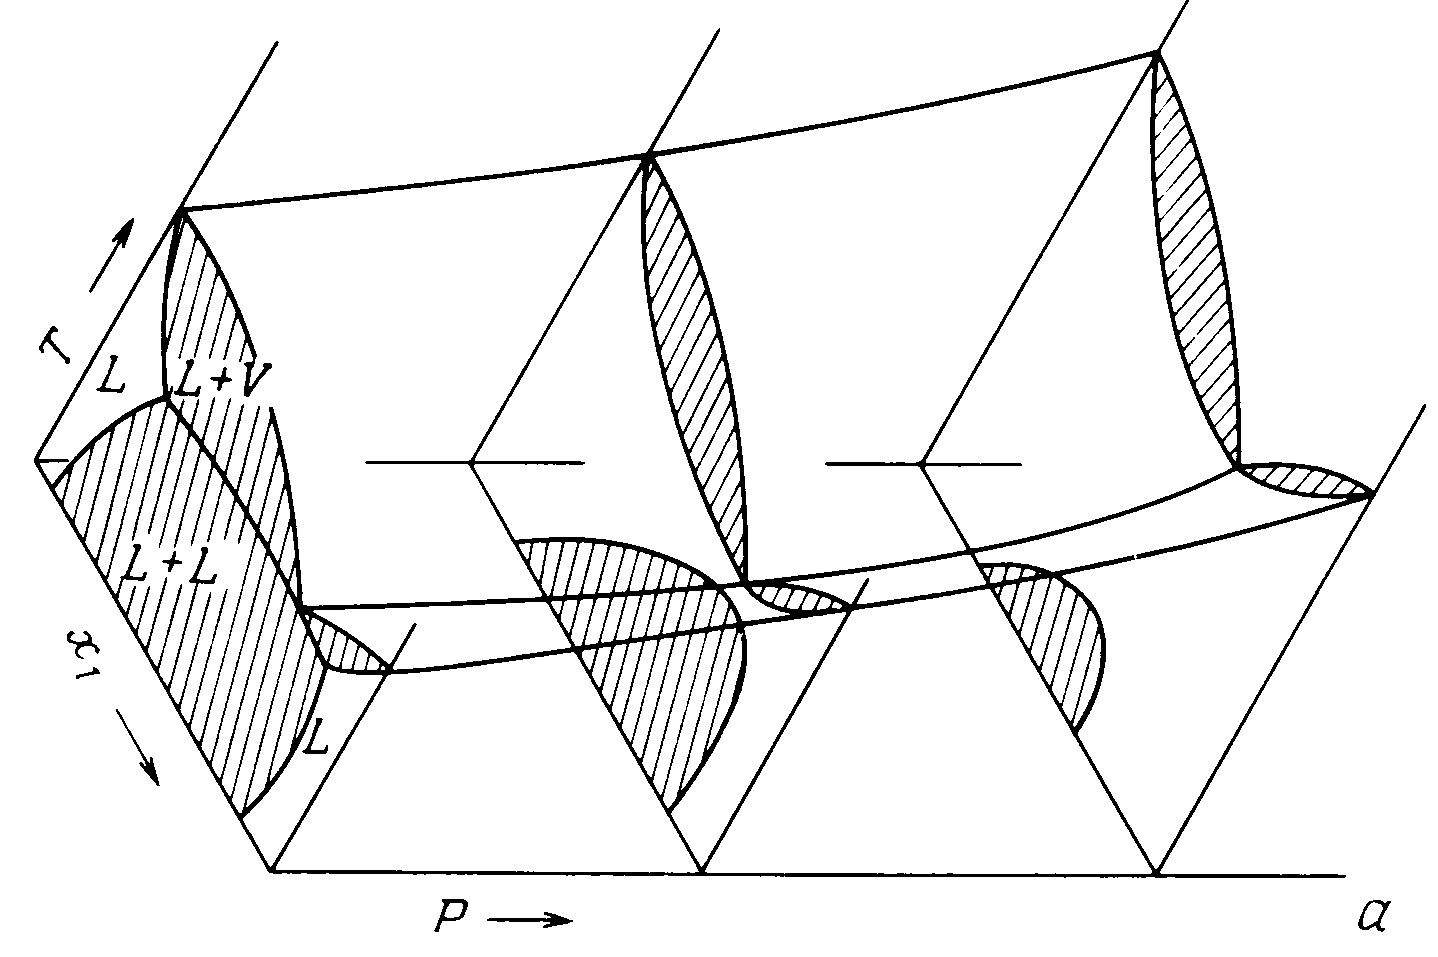
\includegraphics[width=0.8\textwidth]{phase-id-f2.png}
	\end{center}
	\caption{Трехмерная фазовая диаграмма бинарной смеси} \label{fig:phase-id.f2}
\end{figure}

Обычно используют следующие виды диаграмм:
\begin{itemize}
\item в виде изобарических сечений $(p = const)$, которые демонстрируют влияние $Т$ и общего состава смеси на состояние фаз системы (пример такой диаграммы для бинарной смеси представлен на рисунке \cref{fig:phase-id.f3}); 
\item в виде изотермических сечений $(Т = const)$, которые демонстрируют влияние $p$ и общего состава смеси на состояние фаз системы;
\item в виде изоплет (диаграммы постоянного состава), которые демонстрируют влияние $p$ и $Т$ на состояние фаз системы при постоянном составе смеси.	
\end{itemize} 

При построении диаграммы для удобства обычно ограничиваются показом отношений между определенным числом фаз, например пар~-- жидкость, жидкость~-- жидкость, жидкость~-- твердая фаза. Для решения практических задач необходимы лишь ограниченные области $Т$ и $p$, число рассматриваемых фаз также ограничено. При проектировании большинства процессов химической технологии наибольшей интерес представляет набор диаграмм для систем пар~-- жидкость. В этом случае, например диаграмма фазового равновесия (рисунок \cref{fig:phase-id.f3}) является избыточной, так как интерес представляет только ее верхняя часть, где представлена система пар~-- жидкость. 

\begin{figure}
	\begin{center}
		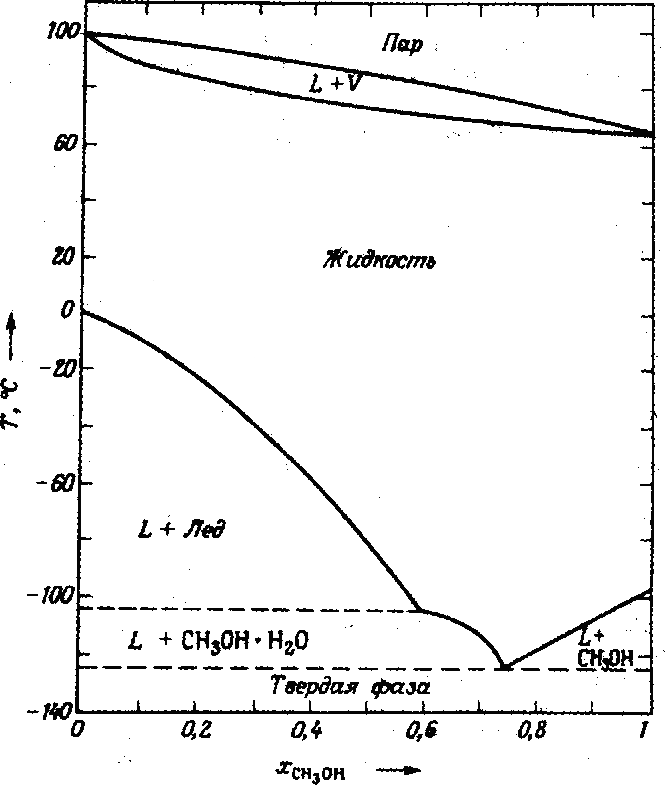
\includegraphics[width=0.5\textwidth]{phase-id-f3.png}
	\end{center}
	\caption{Диаграмма фазового равновесия (пар – жидкость – твердая фаза) в системе метанол + вода при $p = 0.1 МПа$} \label{fig:phase-id.f3}
\end{figure}

На рисунке \cref{fig:phase-id.f4} представлены основные типы фазовых диаграмм систем пар ~-- жидкость. Представленный вид диаграмм характерен для систем с плавным изменением температур кипения растворов в диапазоне температур между температурами кипения чистых жидкостей, включая системы, подчиняющиеся закону Рауля. Вид этих зависимостей определяется свойствами компонентов смеси. Например, для идеальной смеси зависимость $p-х$ при $T=const$ в соответствии с законом Рауля будет прямой линией.

\begin{figure}
	\begin{center}
		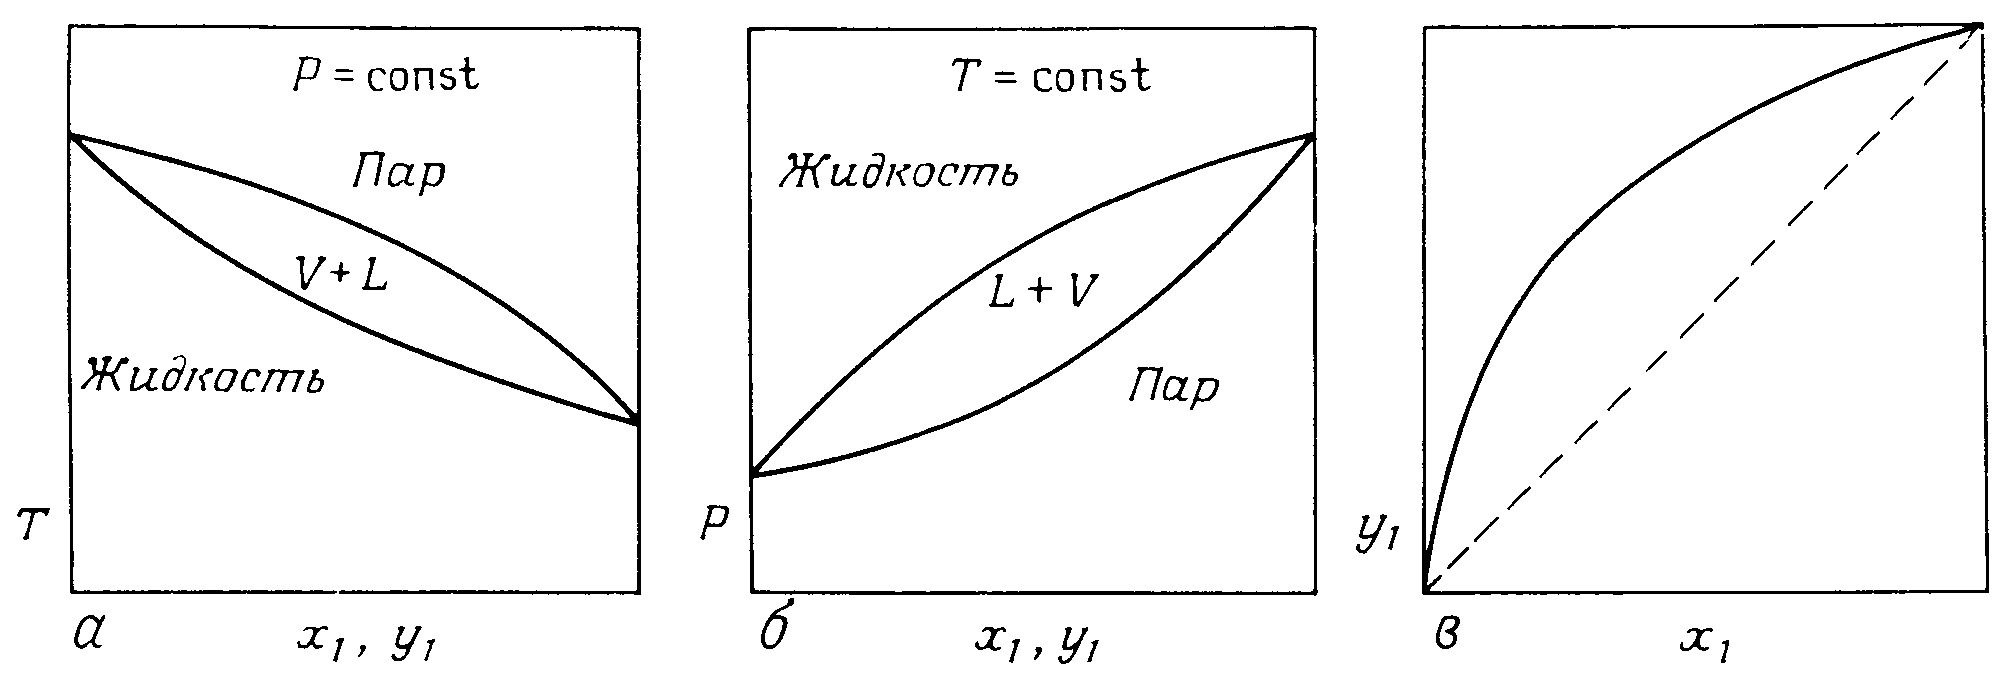
\includegraphics[width=0.9\textwidth]{phase-id-f4.png}
	\end{center}
	\caption{Двухкоординатные фазовые диаграммы $Т – х, у$ (а); $p – х, у$ (б); $х – y$ (в), показывающие паровую и жидкую фазы} \label{fig:phase-id.f4}
\end{figure}

Для технических расчетов наиболее важной является диаграмма $T-x, у$ --- зависимость температур кипения жидкости и конденсации паров от составов жидкой и паровой фаз, так как процессы перегонки в промышленных аппаратах протекают в изобарных условиях. Для проведения расчетов использование данных о фазовом равновесии в графическом виде не всегда удобно, особенно при решении задач оптимизации. В этой связи условия фазовых равновесий удобно представлять в виде системы уравнений, решение которой позволит определить искомые параметры равновесия. 



\subsubsection{Определение условий фазового равновесия}
Условия равновесия двух фаз $n$--компонентной системы при заданной температуре $T$ определяются следующей системой уравнений:
\begin{equation}\label{eq:phas.equi}
\left\lbrace 
\begin{gathered} 
T^{I}=T^{II},\\
p^{I}(T,x_1,x_2,...,x_n-1)=p^{II}(T,y_1,y_2,...,y_n-1),\\
\mu_i^{I}(T,x_1,x_2,...,x_n-1)=\mu^{II}_i(T,y_1,y_2,...,y_n-1),
\end{gathered} 
\right.
\end{equation}
где $\mu$ --- химический потенциал (верхний индекс обозначает фазу, нижний – компонент). Чтобы определить условия фазового равновесия, необходимо решить систему уравнений \eqref{eq:phas.equi}. Численное решение данной системы можно получить, если выражения для химического потенциала и давления представлены в явном виде.
В однокомпонентном случае химический потенциал определяется следующим образом:
\begin{equation}
\int\limits_{\mu^0}^{\mu} d \mu=\dfrac{1}{N} \int\limits_{p^0}^{p} Vdp.
\end{equation}

Отсюда можно получить явный вид для химического потенциала, однако это возможно только если известно уравнение состояния. В случае использования уравнения состояния идеального газа $pV=NRT$ выражение будет иметь вид:
\begin{equation} \label{eq:phase.muid}
	\mu(T,p)=\mu^0(T)+RT \ln (p),
\end{equation}
где $\mu^0(T)$ --- химический потенциал идеального газа при единичном давлении. В случае смеси выражение \eqref{eq:phase.muid} будет иметь следующий вид:
\begin{equation} \label{eq:phase.muidi}
	\mu_i (T,p,x) = \mu_i^0(T) + RT \ln(p_i),
\end{equation}
где $p_i=p x_i$ --- парциальное давление компонента $i$ в смеси.

Для систем, не подчиняющихся уравнению идеального газа вводится понятие летучести (фугитивности): $f=p \gamma_f$ ($f_i=p_i \gamma_{f_i}$), где $\gamma_f$ --- коэффициент летучести (фугитивности), который зависит от $T$, $p$ и состава в случае смеси. Выражение химического потенциала в этом случае запишется следующим образом:
\begin{equation} \label{eq:phase.mureal}
	\mu_i (T,p,x) = \mu_i^0(T) + RT \ln(f_i).
\end{equation}
В случае идеального газа $\gamma_f=1$.
Выражения \cref{eq:phase.muid,eq:phase.muidi,eq:phase.mureal} записаны в случае, когда в качестве системы отсчета для химического потенциала выбрано состояние идеального газа $\mu^0(T)$, что не всегда удобно. Кроме того, коэффициент летучести (фугитивности) может быть определен, только если известно уравнение состояния реального вещества. 

В качестве системы отсчета для жидких смесей часто выбирают химический потенциал чистой жидкости  при тех же $p$ и $T$, что и раствор. В этом случае выражение химического потенциала для жидкой смеси запишется в виде:
\begin{equation}
	\mu_i(T,p,x)=\mu_i^0(T,p)+R T \ln (a_i),
\end{equation}
где $а_i$ --- активность, величина, учитывающая концентрационную зависимость химического потенциала компонентов реального раствора:
\begin{equation}
	a_i=\gamma_i x_i,
\end{equation}
где $\gamma_i$ --- коэффициент активности компонента $i$, в случае идеального раствора $\gamma_i =1 $.

Необходимо отметить, что стандартная часть химического потенциала (первое слагаемое) не зависит от концентрации (см. уравнения \cref{eq:phase.muid,eq:phase.muidi,eq:phase.mureal} ), концентрационная зависимость учитывается вторым слагаемым.

Теперь первое уравнение условий фазового равновесия пар~-- жидкость \eqref{eq:phas.equi} можно записать в виде:
\begin{equation}
	\mu_i^0(T)+RT \ln (f_i)=\mu_i^0(T,p)+ R T \ln (a_i),
\end{equation}
откуда после преобразований можно получить следующее выражение, связывающее концентрации в фазах:
\begin{equation} \label{eq:phase.yreal}
	y_i=\dfrac{f_i^0 \gamma_i x_i}{\gamma_{f_i} p},
\end{equation}
где $f_i^0$ --- летучесть (фугитивность) чистого компонента $i$ при заданных $Т$ и $p$. 
По правилу фаз Гиббса двухфазная система имеет $n$ степеней свободы:
\begin{equation*}
	С=К-Ф+2=n-2+2=n.
\end{equation*}

Для $n$ независимых параметров, полностью определяющих состояние системы, обычно выбирают $n-1$ концентраций в жидкой фазе и $p$ или $Т$.

Следовательно, для определения состава паровой	 фазы и $p$ достаточно системы, состоящей из $n$ уравнений вида \eqref{eq:phase.yreal}, определяющих концентрации в паровой фазе, дополненной выражением
\begin{equation}
	\sum\limits_{i=1}^{n} y_i =1.
\end{equation}

Данная система уравнений может быть упрощена, если принять, что:
\begin{itemize}
	\item паровая фаза подчиняется  уравнению состояния идеального газа, т.е. ${\gamma_f}_i$;
	\item при небольших давлениях значение летучести близко к давлению насыщенных паров чистого компонента $f_i^0 \approx p^0_i (T)$.
\end{itemize}
В итоге получим:
\begin{equation} \label{eq:phase.yapp}
y_i=\dfrac{p_i^0 \gamma_i x_i}{ p}
\end{equation}
Систему уравнений \eqref{eq:phase.yapp} необходимо дополнить зависимостью коэффициента активности $\gamma_i$ от $T$, $p$ и состава, а также зависимостью давления насыщенных паров чистых компонентов от температуры. 

Для случая идеальной смеси ($\gamma_i=1$), находящейся в равновесии с идеальным паром, система \eqref{eq:phase.yapp} сводится к известному закону Рауля:
\begin{equation}
	p_i=p_i^0(T) x_i.
\end{equation}

Общее давление системы запишется в виде:
\begin{equation}\label{eq.phase.sump}
	p=\sum\limits_{i=1}^{n} p_i=  \sum\limits_{i=1}^{n} p_i^0 (T) x_i.
\end{equation}

\subsubsection{Модели для описания давления паров чистых компонентов}


Для описания давления насыщенных паров чистых жидкостей используют различные корреляции \cite{yelles1989,rid1982}:
\begin{itemize}
	\item Клапейрона $\ln(p_i^0(T))=A-\frac{B}{T}$;
	\item Антуана $\ln(p_i^0(T))=A-\frac{B}{T+C}$;
	\item Риделя $\ln(p_i^0(T))=A-\frac{B}{T}+C \ln(T)+D T^2$;
	\item Миллера $\ln(p_i^0(T))=A-\frac{B}{T}+C T+D T^3$;
	\item Ренкина $\ln(p_i^0(T))=A-\frac{B}{T}+С T^2$;
	\item Кеэгоу $\ln(p_i^0(T))=A+\frac{B}{T}+С T+BT^2$;
	\item Реде $\ln(p_i^0(T))=\frac{AT}{T+B}$.
\end{itemize}
где $A$,$B$,$C$,$D$ --- параметры.

Используя систему уравнений \eqref{eq:phase.yapp} совместно с уравнением насыщенных паров, можно определить условия фазового равновесия системы жидкость ~-- пар для идеальной смеси, на основе которых построить соответствующие фазовые диаграммы. 
Алгоритм определения условий фазовых равновесий системы пар ~-- жидкость для идеальной смеси () будет выглядеть следующим образом:
\begin{itemize}
	\item при $T = const$: определяют давления насыщенных паров чистых веществ од одному из представленных выше уравнений, через которые, по выражению \eqref{eq.phase.sump} при известных концентрациях в жидкой фазе рассчитывают  $p$ в системе, а по выражению  \eqref{eq:phase.yapp} --- концентрации в паровой фазах;
	\item при $p = const$: необходимо определить температуру системы $Т$ при фиксированной концентрации в жидкой фазе путем решения нелинейного уравнения для давления в системе \eqref{eq.phase.sump} с учетом выражения для описания давления насыщенных паров. Далее по выражению \eqref{eq:phase.yapp} определяют концентрации в паровой фазе.
\end{itemize}

\subsubsection*{Модели для описания коэффициента активности}
Для большинства смесей закон Рауля представляет собой не более чем грубую аппроксимацию. В действительности же для реальных систем парциальное давление будет отличаться от давления, определенного по закону Рауля:
\begin{equation}
p_i=\gamma_i p_i^0 x_i
\end{equation}
где  - коэффициент активности компонента i. Соответственно давление системы запишется в следующем виде:
\begin{equation} \label{eq.phase.pressgam}
p=\sum\limits_{i=1}^{n} p_i=\sum\limits_{i=1}^{n} \gamma_i p_i^0 x_i
\end{equation}

В этом случае для расчета условий фазового равновесия, кроме давления паров чистого компонента при заданной температуре ($T$), необходимо определять коэффициенты активности в зависимости от температуры, давления и состава.
Истинные коэффициенты активности определяют по данным измерений фазового равновесия ($p$, $T$, $х$,$ у$) \cite{kogan1,kogan2} . При отсутствии этих экспериментальных данных коэффициенты активности также можно рассчитать, используя универсальные уравнения состояния, применимые как для жидкой, так и для паровой фазы. Однако в настоящее время подобные уравнения состояния охватывают лишь немногие группы веществ. Так, уравнения Соава и уравнения, аналогичные уравнению Бенедикта-Уэбба-Рубина, разработаны для класса легких углеводородов и нескольких других газов \cite{rid1982}. Поэтому для определения коэффициентов активности широко используют различные модели.

Для корреляции коэффициентов активности с составом смеси, давлением и температурой предложено много уравнений \cite{rid1982,yelles1989}. Некоторые из них имеют более или менее разработанное теоретическое обоснование, другие являются чисто эмпирическими. В настоящее время наиболее известны пять различных видов корреляций коэффициентов активности (Маргулеса, Ван Лаара, Вильсона, NRTL, UNIQUAC). Поскольку преимущества какого-либо одного метода не всегда явно выражены, на практике следует исходить из имеющегося опыта и аналогий. Также следует учитывать, что для модели Маргулеса и ван Лаара не подходят для описания многокомпонентных смесей.

Ниже для различных моделей приведены выражения избыточной энергии Гиббса и коэффициентов активности.
\begin{itemize}
	\item Уравнение Маргулеса
	
	Выражение избыточной энергии Гиббса двухкомпонентных смесей:
	\begin{equation}\label{eq.phase.gemarg}
	\frac{G^{ex}}{RT}=x_1 x_2 (A_{21} x_1+ A_{12} x_2)
	\end{equation}
	где $A_{12}$ и $A_{21}$ --- параметры модели.
	
	Выражения для коэффициентов активности:
	\begin{equation} \label{eq.phase.ga1marg}
	\ln(\gamma_1)=(A_{12}+2(A_{21}-A_{12})x_1)x_2^2
	\end{equation}
	\begin{equation} \label{eq.phase.ga2marg}
	\ln(\gamma_2)=(A_{21}+2(A_{12}-A_{21})x_2)x_1^2
	\end{equation}
	
	\item Уравнение Ван Лаара
	
	Выражение избыточной энергии Гиббса двухкомпонентных смесей:
	\begin{equation}\label{eq.phase.gewlar}
	\frac{G^{ex}}{RT}=\dfrac{1}{\dfrac{1}{A_{12} x_1}+ \dfrac{1}{A_{21}x_2}}
	\end{equation}
	где $A_{12}$ и $A_{21}$ --- параметры модели.
	\begin{equation}
	\ln(\gamma_1)=A_{12}\left( \dfrac{A_{21}x_2}{A_{12}x_1 + A_{21} x_2}\right)^2
	\end{equation}
	\begin{equation}
	\ln(\gamma_2)=A_{21}\left( \dfrac{A_{12}x_1}{A_{12}x_1 + A_{21} x_2}\right)^2
	\end{equation}
	
	\item Уравнение Вильсона
	
	Выражение избыточной энергии Гиббса двухкомпонентных смесей:
	\begin{equation}\label{eq.phase.wilson}
	\frac{G^{ex}}{RT}=-x_1 \ln(x_1+\Lambda_{12} x_2)-x_2 \ln(\Lambda_{21} x_1 +x_2)
	\end{equation}
	где $\Lambda_{12}=\frac{V_2^L}{V_1^L}\exp\left(-\frac{\lambda_{12}-\lambda_{11}}{RT} \right)$ и $\Lambda_{21}=\frac{V_1^L}{V_2^L}\exp\left(-\frac{\lambda_{21}-\lambda_{22}}{RT}\right)$,  $V_i^L$ --- молярный объем чистого компонента $i$, $\lambda_{ij}$ --- параметр, характеризующий силу взаимодействия компонентов $i$ и $j$, соответственно выполняется соотношение $\lambda_{ij}=\lambda_{ji}$. В данной работе можно использовать в качестве параметров модули $\Lambda_{12}$ и $\Lambda_{21}$, в данном случае коэффициент активности будет зависеть только от состава жидкой фазы.
	
	\begin{equation}
	\ln(\gamma_1)=-\ln(x_1 + \Lambda_{12} x_2) + x_2 \left( \dfrac{\Lambda_{12}}{x_1 + \Lambda_{12} x_2 } - \dfrac{\Lambda_{21}}{\Lambda_{21} x_1+x_2} \right)
	\end{equation}
	\begin{equation}
	\ln(\gamma_2)=-\ln(x_2 + \Lambda_{21} x_1) + x_1 \left( \dfrac{\Lambda_{12}}{x_1 + \Lambda_{12} x_2 } - \dfrac{\Lambda_{21}}{\Lambda_{21} x_1+x_2} \right)
	\end{equation} 
	
	\item Уравнение NRTL (Non-Random Two-Liquid)
	
	Выражение избыточной энергии Гиббса двухкомпонентных смесей:
	\begin{equation}\label{eq.phase.nrtl}
	\dfrac{G^{ex}}{RT}=x_1 x_2 \left( \dfrac{\tau_{21}G_{21}}{x_1 + G_{21} x_2} + \dfrac{\tau_{12} G_{12}}{G_{12} x_1 +x_2} \right)
	\end{equation}
	где $G_{12}=\exp(-\alpha_{12} \tau_{12})$,  $G_{21}=\exp(-\alpha_{21} \tau_{21})$, $\tau_{12}=\dfrac{g_{12}-g_{22}}{RT}$, $\tau_{21}=\dfrac{g_{21}-g_{11}}{RT}$, $g$ --- параметр взаимодействия между компонентами i и j ($g_{ij}=g_{ji}$), $\alpha_{ij}$ --- параметр непроизвольности ($\alpha_{ij}=\alpha_{ji}$)
	В данной работе в качестве параметров модели можно использовать $\tau_{12}$,$\tau_{21})$, $\alpha_{12}$, в данном случае коэффициент активности будет зависеть только от состава жидкой фазы.
	\begin{equation}
	\ln(\gamma_1)=x^2_2 \left( \tau_{21} \left(\dfrac{G_{21}}{x_1+x_2 G_{21}}\right)^2 + \dfrac{\tau_{12} G_{12}}{(x_2+x_1 G_{12})^2} \right)
	\end{equation}
	\begin{equation}
	\ln(\gamma_2)=x^2_1 \left( \tau_{12} \left(\dfrac{G_{12}}{x_2+x_1 G_{12}}\right)^2 + \dfrac{\tau_{21} G_{21}}{(x_1+x_2 G_{21})^2} \right)
	\end{equation} 
\end{itemize}

Рассмотрим методику определения параметров бинарного взаимодействия в изотермическом случае. В качестве исходной информации выступают экспериментальные данные о фазовом равновесии пар – жидкость $(х, у, Р, Т)$. Процедура определения параметров включает следующие этапы:
\begin{enumerate}
	\item При заданной температуре находят давления паров чистых жидкостей $p_i^0(T)$, используя уравнения Менделеева-Клайперона, Антуана, Риделя или др.
	\item Для всех имеющихся экспериментальных данных рассчитывают коэффициенты активности по уравнениям:
	\begin{equation}
		\gamma_1=\dfrac{y_1 p}{x_1 p_1^0(T)}
	\end{equation}
	\begin{equation}
		\gamma_2=\dfrac{y_2 p}{x_2 p_2^0(T)}
	\end{equation}
	\item По полученным значениям коэффициентов активности рассчитывают избыточную мольную энергию Гиббса $g^E$:
	\begin{equation}\label{eq.phase.expge}
		g^E=RT(x_1 \ln(\gamma_1)+x_2 \ln(\gamma_2))
	\end{equation}
	\item Используя  выражения для избыточной мольной энергии Гиббса (равнения \eqref{eq.phase.gemarg} \eqref{eq.phase.gewlar} \eqref{eq.phase.wilson} \eqref{eq.phase.nrtl} ) подбирают такие параметры моделей, чтобы минимизировать расхождение между рассчитанным по данным выражениям и значениям, определенным по экспериментальным данным \eqref{eq.phase.expge}.
\end{enumerate}

Для оценки точности полученных результатов обычно строят две диаграммы: $y – x$ и $p – x, у$ при некоторой постоянной температуре $Т$. Процедура построения включает следующие этапы:
\begin{enumerate}
\item Используя уравнения \eqref{eq.phase.ga1marg} \eqref{eq.phase.ga2marg}, находят  и  при произвольно выбранных значениях $х$ в диапазоне [0;1].
\item Для каждого выбранного значения х находят соответствующее значение $p$ и $y$, используя выражения \eqref{eq.phase.pressgam} и \eqref{eq:phase.yapp}.
\item На основе полученных данных строят графические зависимости.
\end{enumerate}

Вопросы для самоконтроля:
\begin{enumerate}
	\item Как формулируются условия фазового равновесия многокомпонентных многофазных систем?
	\item Виды уравнений регрессии. Обобщенная регрессия.
	\item Методы определения параметров уравнения регрессии.
	\item Определение остаточной ошибки уравнения регрессии.
	\item Как определяется число независимых параметров, полностью определяющих состояние системы?
	\item Какие существуют типы диаграмм фазового равновесия?
	\item Методы расчета фазовых равновесий при различных термодинамических условиях ($p-x,y$,  $T-x,y$)
	\item В каких случаях применим закон Рауля?
	\item Способы определения коэффициентов активности?
	\item Какие данные необходимы при определении параметров модели для описания коэффициентов активности?
\end{enumerate}
\laborator{Определение фазовой диаграммы вещества на основе аналитического уравнения состояния}

\goal{на основе данных по свойствам вещества в критической точке определить параметры уравнения состояния Ван дер Ваальса; с помощью данного уравнения произвести расчеты фазовой диаграммы и давления насыщенных паров вещества; результаты представить графически.}

\subsubsection{Теория}
Аналитическое уравнение состояния представляет собой соотношение между давлением, температурой и мольным объемом. В настоящее время существует много различных форм такой связи. Одним из первых аналитических уравнений состояний, которое было предложено еще в 19 веке, является уравнение Клапейрона – Менделеева:
\begin{equation}\label{eq:eos.ideal}
	p V= N R T,
\end{equation}
где $p$ --- давление газа; $T$ --- абсолютная температура; $V$ --- объем, занимаемый газом; $R$ --- универсальная газовая постоянная; $N$ --- число молей газа. Данное уравнение называют также уравнением идеального газа. 

Оказалось, что для большинства реальных газов, например $\mathrm{CO_2}$, $\mathrm{N_2}$, $\mathrm{O_2}$, данное уравнение хорошо описывало экспериментально наблюдаемые соотношения между $p$, $V$, $T$ лишь при давлениях до нескольких атмосфер. Кроме того, уравнение \eqref{eq:eos.ideal} становится бесполезным при рассмотрении процесса сжижения газов. Идеальный газ остается газом при всех температурах, его объем можно уменьшать до бесконечно малой величины.
 
Иоханнес Дидерик Ван дер Ваальс (1837–1923 гг.) предложил модификацию уравнения идеального газа, учитывающую особенности реальных газов: влияние сил межмолекулярного взаимодействия и размеры молекул. Межмолекулярное притяжение уменьшает давление по сравнению с тем значением, которое оно имеет для идеального газа, так как силы притяжения между молекулами уменьшают скорость движения молекул, приближающихся к стенкам. Если $p_{real}$ --- давление реального газа, а $p_{id}$ --- соответствующее давление идеального газа, т.е. давление в отсутствие межмолекулярных сил притяжения, то $p_{id}=p_{real}+\delta p$, где $\delta p$ --- поправка, зависящая от плотности числа частиц ($\delta p = a \left(\frac{N}{V} \right)^2$). Объем, занимаемый молекулами, меньше объема контейнера, в который они заключены, так как размеры молекул конечны. Поправка к объему из-за размеров молекул, т.е.  поправка на «исключенный объем», пропорциональна числу молекул, т.е. $V_{id}=V-b N$, где $b$ --- поправка на 1 моль. Модификация уравнения состояния идеального газа \eqref{eq:eos.ideal}, учитывающая силы межмолекулярного взаимодействия предложена Ван дер Ваальсом в 1873 году:
\begin{equation} \label{eq:eos.vdv}
	\left( p+ \dfrac{a N^2}{V^2} \right) (V- Nb) = N R T.
\end{equation}



В этом уравнение постоянная $a$ характеризует силы притяжения между молекулами, а постоянная $b$, пропорциональная размеру молекул, характеризует силы отталкивания, т.е. $a$ и $b$ отражают природу конкретного вещества.

При постоянной температуре $Т$ типичные $p-V$ зависимости, называемые $p-V$~--~изотермами, для газа Ван дер Ваальса представлены на рисунке \ref{fig:eos.vdw}

\begin{figure}[h]
	\begin{center}
		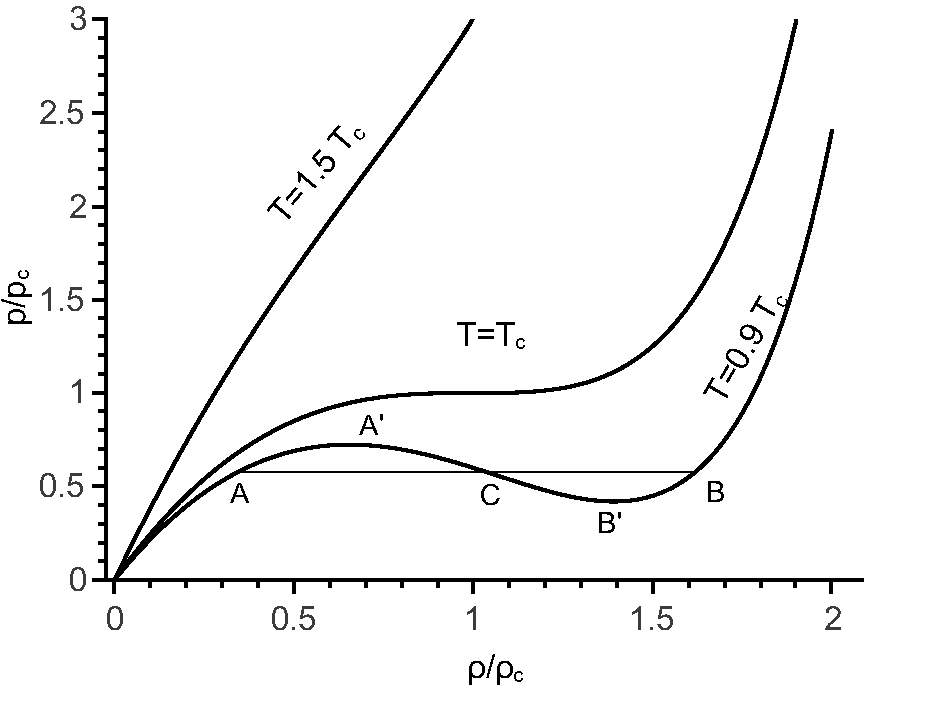
\includegraphics[width=\textwidth]{eos-vdw.pdf}
	\end{center}
	\caption{Изотермы Ван дер Ваальса. При $Т < Т_c$ существует область АА'СВ’В, в которой при заданном давлении $p$ плотность $\rho$ не определяется однозначно уравнением Ван дер Ваальса. В этой области газ превращается в жидкость} \label{fig:eos.vdw}
\end{figure}

Уравнение Ван дер Ваальса свидетельствует о существовании критической температуры $Т_{c}$: при $Т < Т_{c}$ это уравнение описывает кубическую кривую, имеющую два экстремума. В этой области существует фазовый переход пар~-- жидкость. При приближении температуры к $Т_{c}$ эти два экстремума сближаются и, наконец, при $Т=Т_{c}$ сливаются, соответственно переход из газовой фазы в жидкую не происходит, различие между газом и жидкостью исчезает.
При $Т > Т_{c}$ кривая $p-V$ всегда однозначна. Это говорит о том, что в этой области температур не существует перехода в жидкое состояние. Давление и объем, при которых исчезает различие между жидкостью и газом, называют критическим давлением $p_{c}$ и критическим объемом $V_{c}$. Критические параметры $p_{c}$, $V_{c}$ и $Т_c$ могут быть измерены экспериментально и их значения для веществ приведены в справочниках. Критические параметры можно связать с параметрами Ван дер Ваальса $а$ и $b$. 
\begin{equation}
	T_{c}=\dfrac{8 a}{27 R b},
\end{equation}
\begin{equation}
	p_{c}=\dfrac{a}{27 b^2},
\end{equation}
\begin{equation}
	{V_m}_{c}=3 b,
\end{equation}
где ${V_m}_{c}$ --- мольный критический объем. Значения постоянных $a$ и $b$ для многих газов приведены в справочной литературе \cite{rid1982}.

Так как для каждого газа существуют свои критические параметры $p_{c}$, $V_{c}$ и $T_{c}$, то это позволяет ввести безразмерные переменные состояния:
\begin{equation}
	T_{r}=\dfrac{T}{T_{c}},
\end{equation}
\begin{equation}
	p_{r}=\dfrac{p}{p_{c}},
\end{equation}
\begin{equation}
	{V_m}_{r}=\dfrac{V_m}{{V_m}_{c}}.
\end{equation}

Если уравнение Ван дер Ваальса записать в приведенном виде, то получится следующее универсальное уравнение, применимое для любых газов:
\begin{equation} \label{eq:eos.vdvb}
	p_r=\dfrac{8 T_r}{2 {V_m}_r-1}-\dfrac{3}{{V_m}_r^2}.
\end{equation}
Уравнение \eqref{eq:eos.vdvb} в большинстве случаев подтверждается экспериментально. Это означает, что приведенные давления всех газов имеют одно и то же значение при заданном приведенном объеме и приведенной температуре. Этот факт получил название закона соответственных состояний. Согласно этому закону, предполагается, что приведенные свойства (приведенное свойство представляет собой отношение свойство / свойство в критической точке) всех газов и жидкостей по существу одинаковы.

В настоящее время существуют более точные уравнения состояния (Редлиха~-- Квонга, Бенедикта~-- Уэбба~-- Рубина и др.) \cite{rid1982,yelles1989}, но все же следует отметить, что уравнение Ван дер Ваальса до сих пор полезно для создания хоть и приближенного, но простого аналитического представления о поведении реального газа и жидкостей.

Наличие уравнения состояния для вещества позволяет производить расчеты термодинамических свойств вещества, в том числе и его фазовых диаграмм. Расчет диаграмм осуществляется из условий фазового равновесия, записанного для исследуемой системы. Например, для однокомпонентной двухфазной системы, находящейся при заданной температуре $Т$, эти условия имеют вид
\begin{equation}\label{eq:oes.equi}
\left\lbrace 
\begin{gathered} 
T^{I}=T^{II},\\
p^{I}(T,\rho)=p^{II}(T,\rho),\\
\mu_i^{I}(T,\rho)=\mu^{II}_i(T,\rho),
\end{gathered} 
\right.
\end{equation}
где $\mu$ --- химический потенциал, $\rho$ --- плотность; одним и двумя штрихами обозначены равновесные фазы. Численный алгоритм решения данной системы уравнений заключается в определении плотностей паровой и жидкой фаз, обеспечивающих равенство при заданной температуре давлений и химических потенциалов. Соответственно для реализации данного алгоритма необходимо иметь соответствующие выражения для давления и химического потенциала.

Давление в системе определяется использованием соответствующего уравнения состояния вещества (например, уравнения \eqref{eq:eos.vdv}). Химический потенциал, термодинамически связан с давлением и, следовательно, с уравнением состояния: 
\begin{equation}
	\int\limits_{mu^0}^{\mu} d \mu = \dfrac{1}{N} \int\limits_{p^0}^{p} V dp,
\end{equation}
откуда можно получить явное выражение для химического потенциала, которое для систем, не подчиняющихся уравнению состояния идеального газа, запишется в виде:
\begin{equation}
	\mu(T,p)=\mu^0(T)+R T \ln (f)=\mu^0 (T) + R T \ln (p \gamma_f),
\end{equation}
где $f=p \gamma_f$ --- фугитивность (летучесть) для чистого вещества ( $\gamma_f$ --- коэффициент фугитивности).

Коэффициент фугитивности $\gamma_f$ зависит от температуры и давления для чистого вещества (а также еще и от состава в случае смеси) и может быть определен через уравнение состояния вещества. Выражение для коэффициента фугитивности чистого вещества имеет следующий вид
\begin{equation}\label{eq:eos.lngam}
	\ln (\gamma_f) = (Z_V -1) - \int\limits_{\infty}^{V} {\dfrac{A_V-1}{V} d V} -\ln(Z_V),
\end{equation}
где $Z_V$ --- коэффициент  сжимаемости, характеризующий отклонение от идеального газа:
\begin{equation} \label{eq:eos.zv}
	Z_V=\dfrac{p V}{N R T}.
\end{equation}

Для идеального газа $Z_V=1$. Для реальных газов $Z_V$ обычно меньше единицы, за исключением области очень высоких температур и давлений. Для жидкости коэффициент сжимаемости обычно много меньше единицы.

Коэффициент фугитивности для вещества получается подстановкой соответствующего уравнения состояния (например, уравнения \eqref{eq:eos.vdv}) в выражение \eqref{eq:eos.lngam} с учетом \eqref{eq:eos.zv}. Само выражение \eqref{eq:eos.lngam} справедливо для любых веществ. 

\subsubsection{Задание:}
С помощью аналитического уравнения состояния Ван дер Ваальса произвести расчеты фазовой диаграммы вещества и давления насыщенных паров согласно своему варианту (таблица \ref{tab:eos.task}). Сравнить графически результаты расчета с экспериментальными данными.
\begin{table}[h]
	\caption{Свойства веществ в критической точке}
	\label{tab:eos.task}
	\begin{tabularx}{\textwidth}%{|X|X|X|X|X|X|X|}
		{|p{\dimexpr 0.1\linewidth-2\tabcolsep}
		|p{\dimexpr 0.25\linewidth-2\tabcolsep}
		|X
		|X
		|X
		|X
		|X|
		}
		\hline
		№ Варианта & Вещество  & $M$, $\frac{г}{моль}$  & $T_{c}$, К  & $p_{c}$, атм  & $V_{c}$, ${\frac{см^2}{моль}}$ & $T_{тр}$, К  \\ \hline \hline
		1 & Аргон (Ar)  & 39.948  & 150.8 & 48.1 & 74.9 & 83.81 \\ \hline
		2 & Неон (Ne) & 20.183 & 44.4 & 27.2 & 41.7 & 24.66 \\ \hline
		3 & Криптон (Kr) & 83.8 & 209.4 & 54.3 & 91.2 & 115.78 \\ \hline
		4 & Кислород ($\mathrm{O_2}$) & 31.999 & 154.6 & 49.8 & 73.4 & 54.36\\ \hline
		5 & Азот ($\mathrm{N_2}$) & 28.013 & 126.2 & 33.5 & 89.5 & 63.15 \\ \hline
		6 & Ксенон (Xe) & 131.3 & 289.7 & 57.6 & 118 & 161.36 \\ \hline
		7 & Метан ($\mathrm{CH_4}$) & 16.043 & 190.6 & 45.4 & 99 & 90.7 \\ \hline
		8 & Хлор ($\mathrm{Cl_2}$) & 70.906 & 417 & 76 & 124 & 172.17 \\ \hline
		9 & Оксид углерода (CO) & 28.011 & 132.9 & 34.5 & 93.1 & 68 \\ \hline
		10 & Диоксид углерода ($\mathrm{CO_2}$) &44.01 & 304.2 & 72.8 & 94 &	216.55 \\ \hline
	\end{tabularx}
\end{table}
	
	Уравнение Ван дер Ваальса в переменных плотностей и температур имеет вид:
	\begin{equation*}
		p(\rho,T)=\dfrac{\rho R T}{1-\rho b} - a \rho^2,
	\end{equation*}
	где $a$ и $b$ --- коэффициенты, которые определяются следующим образом:
	\begin{equation*}
		a=\dfrac{9 R T_{crit}}{8 \rho_{crit}},
	\end{equation*}
	\begin{equation*}
		b=\dfrac{1}{3 \rho_{crit}}.
	\end{equation*}
	Коэффициент фугитивности в переменных плотностей и температур запишется в виде:
	\begin{equation*}
		\ln(\gamma_f)=Z_V(\rho,T)-1+\int_{0}^{\rho} \dfrac{Z_V(\rho,T)}{\rho} d\rho -\ln(Z_V(\rho,T)
	\end{equation*}
	$Z_V(\rho,T)=p/{\rho R T}$ --- коэффициент сжимаемости.

Вопросы для самоконтроля:
\begin{enumerate}
\item Что понимают под уравнением состояния?
\item В чем отличие уравнения Ван дер Ваальса от уравнения Клапейрона~-- Менделеева?
\item Как формулируются условия фазового равновесия однокомпонентной системы?
\item Что такое критическая точка на диаграмме состояния вещества?
\end{enumerate}

\laborator{Проектный и поверочный расчет абсорбера}

\goal для заданной модели структуры потока по жидкой и газовой фазам составить математическую модель процессов физической и химической абсорбции; на основе полученных моделей провести моделирование данных процессов в абсорбере, заполненном насадочными контактными элементами; результаты представить графически (в виде кривых равновесия и изменения концентрации абсорбтива по высоте аппарата в газовой и жидкой фазах).

\subsubsection{Теория}
Абсорбцией называется избирательное поглощение компонентов паровых или газовых смесей жидким поглотителем. Различают физическую абсорбцию и хемосорбцию.

При физической абсорбции растворение газа не сопровождается химической реакцией (или, по крайней мере, эта реакция не оказывает заметного влияния на процесс). В данном случае парциальное давление распределяемого компонента в газовой фазе превышает равновесное и его поглощение происходит до тех пор, пока его парциальное давление в газовой фазе будет выше равновесного давления над раствором. Физическая абсорбция обычно обратима. На этом свойстве абсорбционных процессов основано выделение поглощенного газа из раствора --- десорбция.

При хемосорбции абсорбируемый компонент связывается в жидкой фазе в виде химического соединения. Химическая реакция может быть как обратимой, так и необратимой. При необратимой реакции равновесное давление компонента над раствором становится близким к нулю и соответственно возможно его более полное извлечение из газовой фазы. При обратимой реакции давление компонента над раствором будет больше, чем при необратимой реакции, но меньше, чем в случае процесса физической абсорбции.

Участвующие в процессе абсорбции рабочие агенты имеют следующие названия:
абсорбтив --- распределяемый компонент газовой фазы, переходящий в жидкую;
инерт (инертный газ) -- компонент газовой смеси, не переходящий границу раздела фаз;
абсорбент --- жидкий поглотитель.

При абсорбционных процессах массообмен происходит на поверхности соприкосновения фаз. Поэтому абсорбционные аппараты должны иметь развитую поверхность соприкосновения между газом и жидкостью. Абсорбционные аппараты подразделяют на две групп:
\begin{itemize}
\item аппараты с непрерывным контактом фаз;
\item аппараты со ступенчатым контактом фаз.
\end{itemize}

В промышленности наибольшее распространение получили насадочные абсорберы, относящиеся к первой группе. В насадочных аппаратах жидкость стекает по поверхности загруженной в абсорбер насадки из тел различной формы (кольца, кусковой материал и т.д.). Для данных аппаратов поверхность контакта определяется геометрической поверхностью элементов насадки и гидродинамическим режимом работы колонны.

В насадочной колонне контакт фаз осуществляется непрерывно. Данное обстоятельство приводит к необходимости использования для математического описания насадочных колонн дифференциальных уравнений, определяющих изменение концентрации распределяемого компонента в потоках по высоте колонны. Это соответственно позволяет определить изменение движущей силы процесса по высоте аппарата.
\begin{wrapfigure}{H}{0.5\textwidth}
	\begin{center}
		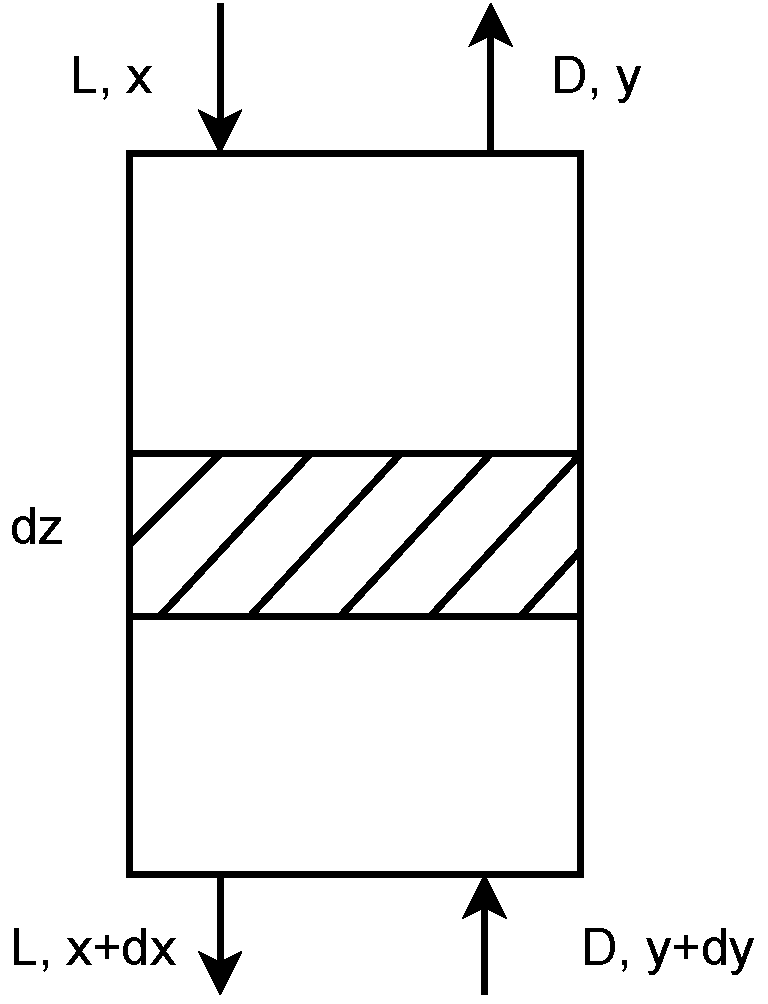
\includegraphics[width=0.48\textwidth]{flowscheme.pdf}
	\end{center}
	\caption{ Схема проведения процесса абсорбции (противоточная)} \label{fig:mass.sheme}
\end{wrapfigure}

Математическое описание процесса физической абсорбции одного компонента в предположении, что движение потоков газа и жидкости описываются гидродинамическими моделями идеального вытеснения, будет состоять из системы двух дифференциальных уравнений, определяющих распределение его концентрации в потоках газа и жидкости. Для расчетов систему координат удобно расположить в верхней части аппарата (рисунок \ref{fig:mass.sheme}), так как в этом случае известны граничные условия: конечная концентрация абсорбтива в газе (степень извлечения задается в исходных данных); начальная концентрация абсорбтива в абсорбенте (принимается равной нулю или задается в исходных данных). В этом случае уравнения материального баланса по распределяемому компоненту для элементарного объема  запишутся следующим образом:
\begin{equation}
	L X - L(X +dX) + K_Y a (Y-Y^*(X))Sdz=0, 
\end{equation}
\begin{equation}
	G(Y-dY)-K_Y a (Y-Y^*(X))Sdz- GY=0,
\end{equation}
где $G$, $L$ --- массовый расход инертного носителя и абсорбента соответственно; $Y$, $X$ --- относительные массовые концентрации абсорбтива в газовой [кг А/кг В] и жидкой фазах [кг А/кг C] соответственно (А --- абсорбтив; В --- инертный газовый носитель; С --- абсорбент); $Y^*$ --- равновесная концентрация абсорбтива в газовой фазе [кг А/кг В]; $S$ --- площадь поперечного сечения аппарата; $а$ --- удельная поверхность контакта фаз; $K_Y$ --- поверхностный коэффициент массопередачи. Таким образом, математическая модель процесса физической абсорбции одного компонента запишется в следующем виде:
\begin{equation}
\left\lbrace 
\begin{gathered} 
\dfrac{dX}{dz}=\dfrac{S}{L} K_Y a (Y-Y^*(X)),
\\
\dfrac{dY}{dz}=\dfrac{S}{G} K_Y a (Y-Y^*(X)).
\end{gathered} 
\right.
\end{equation}

В случае процесса хемосорбции химическая реакция, сопровождающая процесс абсорбции, может оказывать существенное влияние на кинетику процесса. При этом скорость процесса абсорбции определяется не только интенсивностью массопереноса, но и скоростью протекания химической реакции. Если реакция идет в жидкой фазе, то часть газообразного компонента переходит в связанное состояние. При этом концентрация свободного (т.е. не связанного химически) компонента в жидкости снижается, что приводит к увеличению движущей силы процесса и соответственно к ускорению процесса абсорбции. В общем случае скорость хемосорбции зависит как от скорости реакции, так и от скорости массопереноса между фазами. В зависимости от того, какая скорость определяет общую скорость процесса переноса массы, различают следующие области процессов хемосорбции:
\begin{itemize}
	\item кинетическую – скорость химического взаимодействия меньше скорости массопереноса, и поэтому лимитирует скорость всего процесса;
	\item  диффузионную – лимитирующей является скорость диффузии компонентов в зоне реакции, зависит от гидродинамических условий в системе и физических свойств;
	\item смешанная (диффузионно-кинетическая) – скорости химической реакции и массопередачи соизмеримы.
\end{itemize}

При моделировании процесса хемосорбции химическую реакцию можно учесть путем введения источника массы, который будет определять скорость образования или исчезновения компонента в элементарном объеме жидкой фазы. Обычно учет химической реакции осуществляется путем введения в математическую модель кинетического уравнения, определяющего скорость реакции. Если рассматривать химическую реакцию, протекающую в процессе хемосорбции, как элементарную:
\begin{equation}
	n_A A + n_B B \rightarrow n_c C,
\end{equation}
где $n$ --- соответствующие химической реакции стехиометрические коэффициенты, то кинетическое уравнение будет выглядеть следующим образом:
\begin{equation}
	r=k X_A^{n_A} X_B^{n_B},
\end{equation}
где $Х$ --- концентрации соответствующих компонентов. В случае, если порядок реакции по каждому из компонентов равен единице ($n_A=n_B=1$),  кинетическое уравнение запишется в виде
\begin{equation}
r=k X_A X_B.
\end{equation}

Данный вид уравнения справедлив, если проводить реакцию при близких концентрациях обоих компонентов. В процессах хемосорбции химически активные поглотители применяют большей частью в виде растворов, состоящих из инертной жидкости (растворителя) и активной части, причем активная часть находится в избытке относительно поглощаемого компонента. При проведении одной и той же реакции, но в условиях большого избытка одного из реагентов, концентрация вещества, находящегося в избытке, практически не изменяется (т.е. можно считать $X_B=const$) и может быть включена в константу скорости. Кинетическое уравнение в этом случае принимает вид
\begin{equation}
r=k' X_A, \quad k'=k X_B.
\end{equation}
В этом случае мы имеем дело с так называемой реакцией псевдопервого порядка.

Уравнение материального баланса в случае хемосорбции соответственно можно записать в виде
\begin{equation}
L X - L(X +dX) + K_Y a (Y-Y^*(X))Sdz-k'X=0, 
\end{equation}
\begin{equation}
G(Y-dY)-K_Y a (Y-Y^*(X))Sdz- GY=0,
\end{equation}

Отсюда математическая модель процесса хемособции одного компонента запишется следующим образом:
\begin{equation}
\left\lbrace 
\begin{gathered} 
\dfrac{dX}{dz}=\dfrac{S}{L} K_Y a (Y-Y^*(X))-k'X,
\\
\dfrac{dY}{dz}=\dfrac{S}{G} K_Y a (Y-Y^*(X)).
\end{gathered} 
\right.
\end{equation}

Что касается константы скорости химической реакции, то она зависит от температуры и, согласно уравнению Аррениуса, может быть выражена с помощью экспоненциальной функции:
\begin{equation}
	k=k_0 e^{\frac{-E_a}{RT}},
\end{equation}
где $k_0$ --- предэкспоненциальный множитель, $E_a$ --- энергия активации, $R$ --- универсальная газовая постоянная, $Т$ --- температура. 

Оценка эффективности работы абсорбера как аппарата для поглощения компонента газовой смеси оценивают с помощью ряда параметров. Основным из них является степень извлечения компонента. Достигаемая степень извлечения зависит от технологического режима и совершенства как самого процесса, так и его аппаратурного оформления. Степень извлечения можно выразить посредством коэффициента извлечения:
\begin{equation}
	\phi =\dfrac{Y_н - Y_к}{Y_н - Y^*(X_н)},
\end{equation}
представляющего собой отношение количества поглощенного компонента к количеству, которое было бы поглощено при наиболее полном извлечении. Другими словами, он показывает количество поглощенного компонента к теоретическому, достигаемому в условиях равновесия между уходящим из абсорбера газом и вводимым компонентом. При полном извлечении $Y_к=0$, $\phi=1$ (при $Х_н=0$), во всех остальных случаях $\phi<1$.
 
При моделировании процессов химической технологии в зависимости от имеющейся входной и выходной информации, поставленных целей все решаемые задачи можно разделить на поверочные, проектные или проектно-поверочные.

Для проектной задачи требуется определить основные размеры аппарата (в случае процессов разделения это число ступеней разделения, теплообменных процессов --- поверхность теплообмена и т.д.) и режимные параметры процесса. Входная информация содержит данные о величине и составе входящих в аппарат потоков, а также ряд требований к выходящим потокам. 

Для поверочной задачи требуется определить величину и состав выходящих из аппарата потоков при заданных входящих потоках, параметрах аппарата (геометрия, схема потоков и др.) и режимных параметрах процесса. Входная информация содержит основные размеры аппарата и параметры процесса, характеристики всех входящих потоков. Выходная информация --- это характеристики выходящих потоков.

Проектно-поверочный расчет объединяет в одном цикле проектный и поверочный расчеты. 

В качестве примера приведем этапы при расчете пленочного абсорбера.
\begin{itemize}
\item Расчет конечной концентрации поглощаемого компонента в газе:
\begin{equation}
	y_к = (1-\phi) y_н
\end{equation}
\item пересчет концентраций в относительно массовые доли:

\item По уравнению Генри рассчитывается коэффициент распределения:
\begin{equation}
	y^*(x)=\dfrac{E x}{p}
\end{equation} 
где E --- коэффициент Генри, p --- давление.

\item Пересчет расхода газовой фазы на условия в абсоорбере:

\item Расчет расхода жидкой фазы:

\item Определение скорости газа
\item Определение диаметра аппарата

\item Расчет объемного коэффициента массопередачи

\end{itemize}
Этапы предварительного расчета:
1. Расчет конечной концентрации $\mathrm{CO_2}$ в газе, перерасчет концентраций в относительно массовые [4, с. 283].
2. Расчет коэффициента распределения m (закон Генри y*=Ex/P) [4, с. 282].
3. Перерасчет расхода газовой фазы [4, с.13] и расчет расхода жидкой фазы [4, с.290].
4. Определение из материального баланса концентрации СO2 в абсорбенте на выходе из аппарата.
5. Определение скорости газа и диаметра аппарата (выбор диаметра из стандартного ряда) [4, с.292].
6. Расчет объемного коэффициента массопередачи [4, с.293].


Вопросы для самоконтроля
\begin{enumerate}
	\item Процессы абсорбции и хемосорбции. Для решения каких практических задач применяют эти процессы?
	\item Что такое процесс десорбции?
	\item Как составляется материальный баланс процессов абсорбции и хемосорбции?
	\item Дайте определение процесса массопередачи и коэффициента, характеризующего его скорость.
	\item Движущая сила процесса абсорбции.
	\item Как провести оценку эффективности работы абсорбера?
\end{enumerate}
\laborator{Лабораторная работа моделирование тепломассообменных процессов}

В связи с тем, что модель идеального вытеснения имеет наибольшую движущую силу, в промышленности наиболее распространение получили аппараты наиболее близкие к данной структуре потока: кожухотрубчатые, "труба в трубе", пластинчатые и другие. На рисунке представлена схема потоков в прямоточном теплообменнике. 

Тепловой баланс холодного теплоносителя:
\begin{equation}\label{eq:tbal-cold}
	G_1 T c_{p1}-G_1 (T_1+\Delta T_1) + q \Delta F=0
\end{equation}
Поток тепла направлен от холодного теплоносителя к горячему, поэтому в выражении теплового баланса будет с отрицательным знаком:
\begin{equation}\label{eq:tbal-hot}
	G_2 T_2 c_{p2} -G_2 (T_2 - \Delta T_2) -q \Delta F =0
\end{equation}

Поток тепла можно выразить уравнением теплопередачи:
\begin{equation}\label{eq:teploper}
	q=K(T_2-T_1)
\end{equation}
где K --- коэффициент теплопередачи. Расписывая площадь поверхности теплопередачи через периметр сечения теплопередачи $P$ и длину элементарного объема $\Delta x$ как $\Delta F = \Delta x P$, с использованием выражения \ref{eq:teploper}, уравнения \ref{eq:tbal-cold} и \ref{eq:tbal-hot} можно переписать в виде системы:

 \begin{equation}
 \left\{
 \begin{aligned}
 &\dfrac{dT_1}{dx}=\dfrac{K(T_2-T_1)P}{G_1 c_{p1}}        \\
 &\dfrac{dT_2}{dx}=-\dfrac{K(T_2-T_1)P}{G_2 c_{p2}}            
 \end{aligned}
 \right.
 \end{equation}

В зависимости от поставленной задачи граничные условия могут задаваться по разному. Обычно известны расходы теплоносителей и температуры на входе теплообменника.

Для противоточного теплообменника можно записать следующую систему дифференциальных уравнений:
 \begin{equation}
 \left\{
 \begin{aligned}
 &\dfrac{dT_1}{dx}=\dfrac{K(T_2-T_1)P}{G_1 c_{p1}}        \\
 &\dfrac{dT_2}{dx}=\dfrac{K(T_2-T_1)P}{G_2 c_{p2}}            
 \end{aligned}
 \right.
 \end{equation}
 
 В случае противоточного направления и известных входящих потоках необходимо решать краевую задачу.
 
 Для плоской стенки коэффициент определяется как:
 \begin{equation}
 	K=\dfrac{1}{\dfrac{1}{\alpha_1} + \sum \dfrac{\delta}{\lambda} + \dfrac{1}{\alpha_2}}
 \end{equation}
 где $\alpha$ --- коэффициент теплоотдачи, $\delta$ --- толщина стенки, $\lambda$ --- коэффициент теплопроводности материала стенки, суммирование $\frac{\delta}{\lambda}$ проводится в случае если стенка состоит из нескольких слоев различного материала. Коэффициент теплоотдачи описывается критериальными уравнениями и зависит от многих факторов: конструкции аппарата, скорости движения жидкости физико-химических свойств. Обычно при решении задачи теплопередачи используются следующие критерии: Рейнольдса $Re=\dfrac{\bar{w} l \rho}{\mu}$, Прандтля $Pr=\dfrac{\mu c_p}{\lambda}$, Грасгофа $ Gr= g l^3 \beta_p \rho^2 \dfrac{\Delta T}{\mu^2}$, где $\bar{w}$ --- усредненная по сечению скорость движения теплоносителя, $l$ --- характерный размер аппарата, $\rho$ --- плотность теплоносителя, $\mu$ --- коэффициент вязкости, $c_p$ --- теплоемкость,  $\lambda$ --- теплопроводность, $g=9.8 м/с$, $\beta_p$ --- коэффициент объемного расширения, $\Delta T$ --- движущая сила теплоотдачи.
  При расчете коэффициентов теплоотдачи трубах в качестве характерного размера при определении критериев подобия выступает эквивалентный диаметр $D_э=\dfrac{4S}{P}$, где $S$ --- площадь сечения, $P$ --- периметр сечения.
 \begin{itemize}
	 \item Теплоотдача в круглых трубах при турбулентном режиме ($Re>10000$):
		 \begin{equation}
		 	Nu=0.021 Re^{0.8} Pr^{0.43} \left( \dfrac{Pr}{Pr_{гр}} \right) ^{0.25} 
		 \end{equation}
	 \item Теплоотдача в круглых трубах при переходном режиме ($2300<Re<10000$):
		 \begin{equation}
		 	Nu=0.008 Re^{0.9} Pr^{0.43}
		 \end{equation}
	 \item Теплоотдача в круглых трубах при ламинарном режиме течения:
		\begin{equation}
			Nu=0.17 Re^{0.33} Pr^{0.43} Gr^{0.1} \left( \dfrac{Pr}{Pr_{гр}} \right)
		\end{equation}
	 \item  Теплоотдача в кольцевом канале:
		 \begin{equation}
			  Nu=0.023 Re^{0.8} Pr^{0.4} \left(\dfrac{D_{вн}}{d_{н}}\right)^{0.45}
		 \end{equation}
		 где $D_{вн}$, $d_н$ --- внутренний и наружный  диаметр кольцевого сечения, характерным размером является $d_н$
	 \item Теплоотдача при перемешивании жидкостей мешалками:
	 \begin{equation}
		Nu=C Re^m Pr^{0.33} \left(\dfrac{\mu}{\mu_{ст}}\right)^{0.14} \dfrac{\lambda}{D}
	 \end{equation}
	 где критерий Рейнольдса определяется как $Re=\frac{ \rho n d_m^2}{\mu}$, $D$ --- диаметр емкости, $n$ --- частота вращения мешалки, $\mu_{ст}$ --- динамический коэффициент вязкости жидкости при температуре стенки змеевика или рубашки, $\mu$ --- коэффициент вязкости при средней температуре жидкости, определяемой $(t_{ср.ж}+t_{ст})/2$. Для аппаратов с рубашками: $C=0.36$, $m=0.67$
\end{itemize}

В предлагаемых задачах можно считать теплофизические свойства не зависящими от температуры, следовательно в первом приближении  $\frac{Pr}{Pr_{ст}}=\frac{\mu}{\mu_{ст}}=1$, $\Delta T$ принять равным 5 С

\laborator{Моделирование реакций в реакторах с различной структурой потоков}

\goal для различных моделей структуры потока составить математическую модель протекающих в аппарате химических реакций; на основе полученных моделей провести моделирование работы реактора; результаты оценки эффективности для различных вариантов аппарата представить графически (в виде зависимости селективности и степени превращения от времени пребывания в аппарате).

Теория
Основными критериями эффективности проведения химических реакций являются конверсия и селективность. 
Конверсия (степень превращения) --- это величина, характеризующая превращение сырья в результате реакции. Она представляет собой отношение общего количества исходного реагента, вступившего в реакцию $m_A^R$ , к количеству реагента, взятого для проведения реакции $m_A^0$:
\begin{equation}\label{eq:rea.alpha}
	\alpha_A = \dfrac{m_A^R}{m_A^0}
\end{equation}
В случае, если в реакцию вступает несколько веществ, конверсию рассчитывают по наиболее ценному веществу.  

Селективность --- это отношение количества исходного реагента, расходуемого на целевую реакцию $m_A^Ц$, к общему количеству реагента, пошедшего на реакцию $m_A^R$:
\begin{equation}\label{eq:rea.s}
	S_B= \dfrac{m_A^Ц}{m_A^R}
\end{equation}

Выход реакции --- отношение количества продукта $m_B^Ц$ к максимальному, теоретически возможному количеству продукта $m_B^{Max}$:
\begin{equation}\label{eq:rea.beta}
	\beta_B=\dfrac{m_B^Ц}{m_B^{Max}}
\end{equation}
Теоретически максимальное значение количества продукта рассчитывается из материального баланса при следующих условиях: скорость побочных реакций равна нулю, обратимые целевые реакции проходят до условий равновесия.

Выбор этих показатели для оценки эффективности связан с тем, что:
\begin{itemize}
	\item в себестоимости процессов химического превращения стоимость сырья составляет порядка 50\ --\ 60\ \%.
	\item энергетические затраты, связанные с нагревом, охлаждением, перемещением сырья и продуктов реакции, зависят от того, сколько сырья приходится возвращать на повторную переработку. При конверсии 100\ \% все сырье пропускается через реактор один раз, при меньшей конверсии часть сырья приходится снова возвращать реактор;
	\item продукты реакции из реактора необходимо разделять и для их разделения потребуется немало разнообразного оборудования, многочисленные циклы нагрев -- охлаждение, испарение -- конденсация... Следовательно, дополнительные затраты энергии, а значит, и средств.
\end{itemize}

Селективность и конверсия подчиняются строгим законам, а именно законам химической термодинамики и кинетики. Это справедливо на этапе создания технологии. Однако когда мы говорим о проектировании аппаратов для реализации данных процессов, то на величину селективности, а особенно степени превращения, большое влияние оказывает время пребывания молекулы вещества в реакторе. Оценочное значение среднего времени пребывания получают из отношения объема реактора к объемному расходу поступающего вещества. В действительности же траектория движения элементов потока в аппарате может быть чрезвычайно сложной, что может приводить к существенным отклонениям времени пребывания конкретного элементарного объема от среднего значения. Структура потоков в аппарате зависит от конструкции реактора и гидродинамических условий. 

При математическом моделировании работы аппаратов используются различные модели структуры потоков, основными из них являются следующие: 
\begin{itemize}
\item модель идеального вытеснения;
\item модель идеального смешения;
\item диффузионная модель;
\item ячеечная модель.
\end{itemize}

Необходимо отметить, что данные модели представляют собой упрощенную картину реальной структуры потоков в аппаратах, которая значительно сложнее. Например, многие химические реакции сопряжены с процессами теплообмена, которые вследствие неоднородности поля температур (наблюдаемой при теплообмене) дополнительно усложняют характер движения элементов потока, например за счет конвективных токов, вызванных естественной конвекцией.

\subsection*{Изотермический реактор идеального вытеснения}
Наибольшее распространение на производстве получили изотермические реакторы непрерывного действия. В них температура поддерживается на постоянном уровне как во времени, так и в пространстве, что обеспечивает постоянство константы скорости химической реакции (на оптимальном уровне) и, следовательно, упрощает задачу проведения процесса. Рассмотрим реактор данного типа, в котором протекают следующие реакции:
\begin{equation*} 
\begin{aligned} 
A+B \xleftrightarrow[k_2]{k_1} C + \Delta H_1\\
C \xrightarrow{k_3} D + \Delta H_2
\end{aligned} 
\end{equation*}
где $k$ --- константы скорости реакции.
Математические модели аппаратов составляются на основе записи уравнений кинетики, материального и теплового баланса. В случае изотермического реактора тепловым балансом можно пренебречь. Для реактора данного типа математические модели для различных структур потока представлены в работе \cite{klinov-mm2009}. Рассмотрим варианты идеализированных моделей реактора.

Изменением температуры можно пренебречь при малых значениях теплового эффекта реакций ($\Delta H_1 \approx 0$, $\Delta H_2 \approx 0$) или компенсации выделенного~/~поглощенного тепла за счет внешнего теплообмена .
В стационарных условиях изменение концентрации компонентов описывается уравнением:
\begin{equation} \label{eq:rea.miv1}
\nu \dfrac{d C_A}{d x} = i
\end{equation}
где $\nu$ --- скорость движения среды, $C_A$ --- концентрация компонента A, $x$ --- длинна реактора, $i$ --- сток или приход массы. В случае отсутствия межфазного массопереноса, сток или приход массы обуславливается только лишь химической реакцией. Компонент А участвует в 1 и 2 (обратимой реакции). В первой реакции компонент А расходуется, следовательно это сток массы и скорость 1 реакции будет со знаком --. Обратная реакция увеличивает концентрация компонента А, и скорость реакции запишем со знаком +. Суммарное выражение изменения концентрации запишется в виде $i=-r_1+r_2$.

Скорость реакции равна произведению константы скорости на концентрацию компонентов, вступающих в реакцию, так скорость первой реакции равна: 
\begin{equation} \label{eq:rea.react1}
r_1=k_1 C_A C_B
\end{equation}
Используя определение скорости $\nu=\frac{d x}{d \tau}$ и выражение \eqref{eq:rea.react1}
перепишем уравнение \eqref{eq:rea.miv1} для описания изменения концентрации в зависимости от времени пребывания компонента в реакторе $\tau$:
\begin{equation}
\dfrac{d C_A}{d \tau} = -k_1 C_A C_B +k_2 C_C
\end{equation}
Составляя аналогичные уравнения для остальных веществ, получим систему дифференциальных уравнений:
\begin{equation}\label{eq:rea.sys1}
\left\lbrace 
\begin{gathered} 
\dfrac{d C_A} {d \tau} = -k_1 C_A C_B +k_2 C_C \\
\dfrac{d C_B} {d \tau} = -k_1 C_A C_B +k_2 C_C \\
\dfrac{d C_C} {d \tau} = k_1 C_A C_B -k_2 C_C - k_3 C_C \\
\dfrac{d C_D} {d \tau} = k_3 C_C \\
\end{gathered} 
\right.
\end{equation}

В результате решения системы уравнений \eqref{eq:rea.sys1} получим концентрации каждого из компонентов в конкретный момент времени. Полученные таким образом векторы решений будут представлять собой зависимость концентраций исходных компонентов и продуктов реакции от времени пребывания в аппарате.

По результатам моделирования можно произвести расчеты показателей конверсии \eqref{eq:rea.alpha}, селективности \eqref{eq:rea.s} и выхода \eqref{eq:rea.beta}, на основе которых производится выбор оптимального типа реактора для проведения процесса. 

\subsection*{Неизотермический реактор идеального вытеснения}
В действительности реакций с нулевым тепловым эффектом практически не существует. Рассмотрим неизотермические реакторы на примере тех же реакций.
Изменение температуры в реакторе идеального вытеснения определяется по выражению:
\begin{equation}\label{eq:rea.dtmiv}
	\nu \rho c_p \dfrac{d T}{d x} = \sum q_i
\end{equation}
где $q_i$ --- подводимый или отводимый поток тепла. Суммарный поток тепла складывается из нескольких составляющих: подвода или отвода теплоты за счет теплоносителя (реакторы с рубашкой, змеевиком и т.д.) и теплоты химических реакций. 

В случае адиабатического реактора все тепло химической реакции идет на изменение температуры в реакторе. Поток тепла за счет химической реакции определяется по выражению:
\begin{equation} \label{eq:rea.qreak}
	{q_r}_q=r_1 \Delta H_1 = k_1 C_A C_B \Delta H_1
\end{equation}

По закону Гесса тепловой эффекта 2 реакции (обратной) будет равен $-\Delta H_1$. Используя определение скорости $\nu=\frac{d x }{d \tau}$ и выражения \cref{eq:rea.qreak,eq:rea.dtmiv} можно записать выражение изменения температуры во времени:
\begin{equation}\label{eq:rea.dtmiv1}
	\dfrac{d T}{d \tau}= \dfrac {k_1(T) C_A C_B \Delta H_1 -k_2(T) C_C \Delta H_1 +k_3(T) C_C \Delta H_2}{\rho c_p} 
\end{equation}
Данным выражением необходимо дополнить систему уравнений \cref{eq:rea.sys1}. Следует заметить, что в выражениях для  неизотермического реактора константа скорости будет функцией температуры и описываться уравнением Аррениуса:
\begin{equation}
	k_i={k_0}_i \exp \left( \dfrac{-E_i}{RT}\right)
\end{equation}
где $k_0$ --- предэкспоненциальный множитель,  $E$ --- энергия активации.

В случае подвода или отвода тепла в выражение \eqref{eq:rea.dtmiv} необходимо добавить член, описывающий тепловой поток $q=K(T-T_T)P$, где $К$ --- коэффициент теплопередачи, $P$ --- периметр сечения поверхности теплопередачи, $T_T$ --- температура теплоносителя. Таким образом изменение температуры можно описать дифференциальным уравнением:
\begin{eqnarray}\label{eq:rea.dtmiv2}
\dfrac{d T}{d \tau}= \dfrac {k_1(T) C_A C_B \Delta H_1 -k_2(T) C_C \Delta H_1 +k_3(T) C_C \Delta H_2}{\rho c_p} + \nonumber \\ + \dfrac{K(T_T-T)P}{\rho c_p} \quad
\end{eqnarray}

Постоянство температуры теплоносителя возможно поддерживать за счет фазового перехода, так, при обогреве реакционной смеси паром, по всей длине реактора температура конденсата будет постоянно. В случае, если температура теплоносителя изменяется по длине реактора, систему дифференциальных уравнений необходимо дополнить изменением температуры теплоносителя. Например если структура потока теплоносителя описывается моделью идеального вытеснения и потоки движутся прямотоком изменение температуры будет записано в виде:
\begin{equation}
	\dfrac{d T_T}{d \tau} = -\dfrac{K(T_T-T)P}{\rho_T {c_p}_T}
\end{equation}
где индексы $T$ --- обозначают свойства теплоносителя.


\subsection*{Изотермический реактор идеального смешения}
В реакторе идеального смешения происходит мгновенное выравнивание полей концентрации и температуры. Уравнения для описания изменения концентрации во времени можно получить исходя из модели идеального вытеснения соответствующей реакции (уравнение \eqref{eq:rea.sys1}) с учетом постоянства концентрации компонентов и температуры в реакторе. Интегрируя уравнение при заданных начальных концентрациях  $C_{0_i}$  для рассматриваемой реакции получим систему алгебраических уравнений:

\begin{equation}\label{eq:rea.syssmis}
\left\lbrace 
\begin{gathered} 
\dfrac{C_A - {C_A}_0} {\tau} = -k_1 C_A C_B +k_2 C_C \\
\dfrac{C_B - {C_B}_0} {\tau} = -k_1 C_A C_B +k_2 C_C \\
\dfrac{C_C - {C_C}_0} {\tau} = k_1 C_A C_B -k_2 C_C - k_3 C_C \\
\dfrac{C_D - {C_D}_0} {\tau} = k_3 C_C \\
\end{gathered} 
\right.
\end{equation}

\subsection*{Незотермический реактор идеального смешения}


%\zd 
 
 
Вопросы для самоконтроля
\begin{enumerate}
	\item По каким критериям оценивается эффективность проведения химических реакций?
	\item Какие факторы оказывают влияние на критерии эффективности проведения химических реакций?
	\item Что понимают под структурой потока в аппарате?
	\item Какие существуют модели структуры потоков?
	\item На основе чего составляются математические модели реакторов?
	\item Как провести сравнение эффективности работы реакторов?
\end{enumerate}
\laborator{Моделирование процесса ректификации бинарной смеси в тарельчатой колонне}

\goal{составить математическую модель процесса ректификации бинарной смеси в тарельчатой колонне; на ее основе разработать алгоритм численного решения и, используя язык программирования Mathcad, провести моделирование колонны.}

\subsubsection{Теория}
Разделение жидких смесей ректификацией на практически чистые компоненты или на фракции различного состава является широко распространенным процессом химической технологии. Разделению подвергаются смеси, состоящие из компонентов с неограниченной и ограниченной взаимной растворимостью. Каждому классу этих смесей соответствуют характерные условия равновесия кипящей жидкой фазы и образующихся из нее паров, отображаемые диаграммами фазового равновесия жидкость~-- пар.

При кипении жидкой смеси концентрация низкокипящего компонента в образующихся парах больше, чем в жидкой фазе. При частичной конденсации образовавшейся паровой фазы, конденсироваться в большей степени будут высококипящие компоненты, а остаток пара будет обогащен низкокипящими компонентами. Это позволяет разделить исходную жидкую смесь с любым числом компонентов на любое число фракций различных составов путем частичного испарения этой смеси и конденсации образующихся паров. Такой процесс называется дистилляцией, получаемые конденсаты – дистиллятами, а неиспарившаяся часть жидкой смеси – кубовым остатком. 

Для более четкого разделения исходной жидкой смеси на узкие фракции или чистые компоненты прибегают к многократному чередованию процессов испарения и конденсации. Этот сложный процесс, называемый ректификацией, осуществляется в колонных аппаратах при противотоке жидкости и пара. Восходящий поток пара при каждом контакте со стекающей жидкой смесью обогащается низкокипящими компонентами за счет частичной конденсации высококипящих и частичного испарения низкокипящих. При достаточном числе таких контактов пар будет уходить из верхнего сечения колонны с преимущественным содержанием низкокипящих, а жидкость уйдет из нижнего сечения колонны с преимущественным содержанием высококипящих компонентов.

Процесс ректификации осуществляется в большинстве случаев в противоточных колонных аппаратах с контактными элементами (насадки, тарелки). Схема типовой ректификационной установки непрерывного действия представлена на рисунке \ref{fig:rect.scheme}.

\begin{figure}[h]
	\begin{center}
		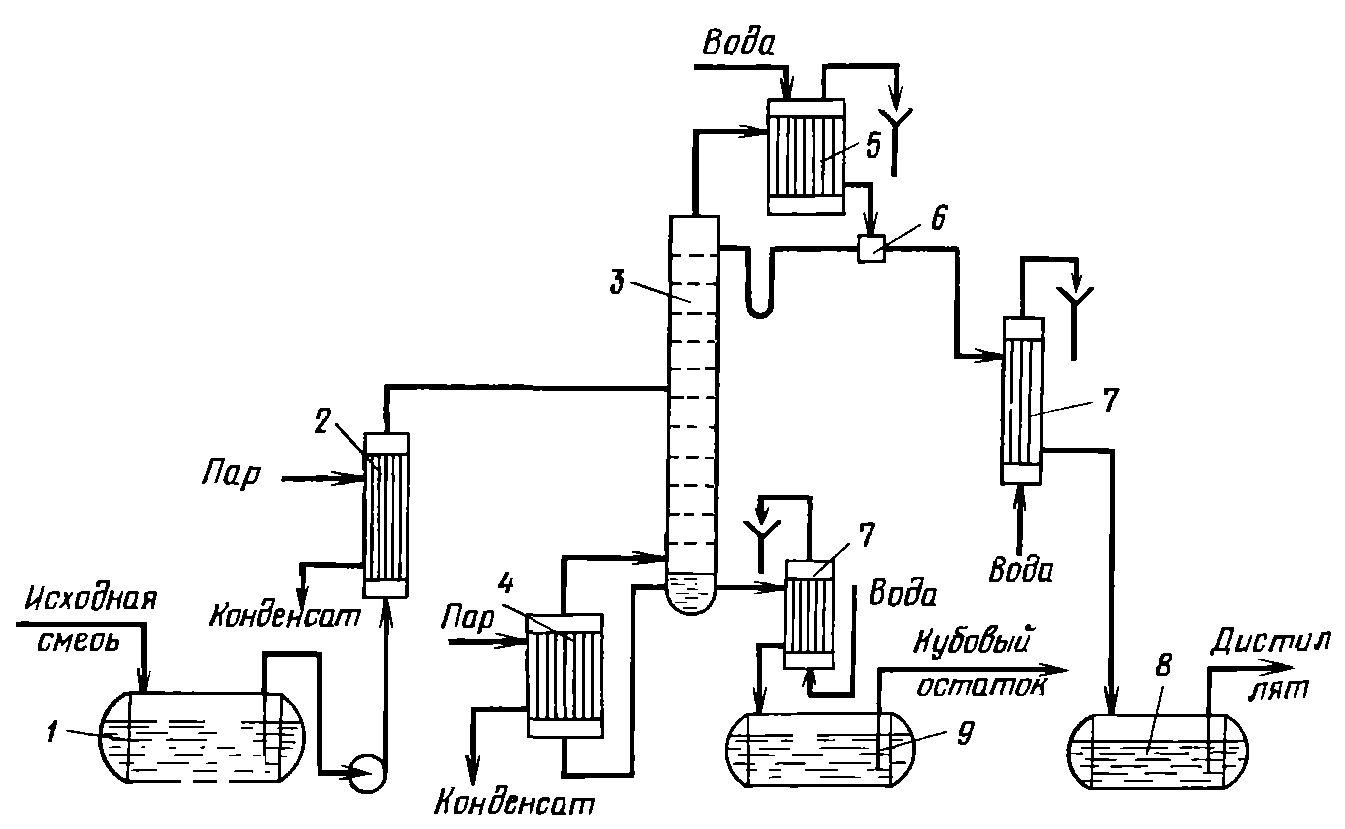
\includegraphics[width=\textwidth]{scheme.png}
	\end{center}
	\caption{Схема ректификационной установки непрерывного действия:1 --- емкость для исходной смеси; 2 --- подогреватель; 3 --- колонна; 4 --- кипятильник; 5 --- дефлегматор; 6 --- делитель флегмы; 7 --- холодильник; 8 --- сборник дистиллята; 9 --- сборник кубового остатка} \label{fig:rect.scheme}
\end{figure}


Исходную смесь подают в то место ректификационной колонны 3, в котором состав жидкой фазы наиболее близок по составу к смеси, поступающей в колонну на разделение. Подача питания обеспечивает непрерывность проведения процесса ректификации. Место ввода исходной смеси, нагретой до температуры кипения в подогревателе 2, называют тарелкой питания, или питательной тарелкой. Положение тарелки питания для ввода исходной смеси специально рассчитывается. Поток пара, поднимающегося по ректификационной колонне, поддерживается испарением кубовой жидкости в кипятильнике 4, а поток жидкости, текущей по колонне сверху вниз, флегмой, образующейся при конденсации выходящих из колонны паров в дефлегматоре 5. Отношение расхода флегмы $Ф$ к расходу отбираемого дистиллята $Р$ называют флегмовым числом $R$ (т. е. $R = Ф/Р$).

Из всей схемы ректификационной установки (рис. \ref{fig:rect.scheme}) при моделировании процесса ректификации рассматриваются только сама ректификационная колонна 3, кипятильник 4 и дефлегматор 5. Данные аппараты оказывают влияние на ход процесса разделения \cite{klinov-mm2009}. Остальное оборудование (в основном это теплообменники) определяется в последующем, исходя из результатов расчета колонны. При технологическом расчете массообменных аппаратов должны быть определены их основные размеры: диаметр, характеризующий производительность аппарата, и рабочая высота, отражающая интенсивность протекающего в нем процесса.

Расчет диаметра аппарата производится по уравнению расхода:
\begin{equation}
	Q=S w_0
\end{equation}
где $Q$ --- объемный расход пара, скорость которого определяет площадь поперечного сечения колонны; $w_0$ --- фиктивная скорость пара; $S$ --- площадь поперечного сечения аппарата. Обычно нижняя часть ректификационной колонны работает при большем орошении по сравнению с верхней, поэтому иногда (для повышения эффективности работы верхней части) необходимо рассчитывать верхнюю и нижнюю части колонны отдельно.

Высота массообменного аппарата определяется в зависимости от того, является контакт фаз в нем непрерывным или ступенчатым. При непрерывном контакте фаз высоту аппарата можно найти на основе уравнения массопередачи или его модификации, выразив высоту аппарата с помощью единиц переноса.

Для расчета высоты аппарата через число ступеней в аппаратах со ступенчатым контактом фаз необходимое число ступеней определяется графическими или аналитическими методами. Графические методы имеют ограничения, так как они применимы только при расчете бинарной ректификации. Аналитические методы применимы как в случае бинарной, так и многокомпонентной ректификации.

Одним из аналитических методов расчета ректификационной колоны является метод расчета от тарелки к тарелке, в котором последовательно определяются расходы материальных потоков и их составы на каждой ступени разделения. В самом простом виде данный метод имеет следующие допущения:
\begin{itemize}
	\item жидкость на тарелке полностью перемешана;
	\item молярные расходы пара и жидкости по колонне не изменяются;
	\item в дефлегматоре и кипятильнике не происходит изменения соответственно состава пара и жидкости.
\end{itemize}

В результате сделанных допущений из уравнения материального баланса и массопереноса для каждого компонента на тарелке получают уравнения, устанавливающие зависимость между составами пара и жидкости покидающими тарелку. 
Спецификой процесса ректификации является сопряженность процессов массо- и теплопереноса, что приводит к некоторым последствиям, усложняющим анализ и расчет данного процесса. Некоторые из них кратко рассмотрены ниже:
\begin{itemize}
	\item иногда возможно существенное изменение физических свойств сред по высоте колонны, что может повлиять не только на скорость массопереноса, но даже и на величину поверхности контакта фаз (ухудшение или улучшение смачиваемости насадки, изменение размеров пузырьков и т.д.). Последнее обстоятельство связано в основном с изменением поверхностного натяжения жидкости как следствие изменения ее состава и температуры;
	\item допущение при анализе и расчете ректификационных колонн равенства молярных теплот испарения компонентов иногда может дать достаточно большие отклонения. Анализ этих возможных эффектов следует проводить в каждом конкретном случае.
\end{itemize}

\begin{wrapfigure}{R}{0.4\textwidth}
	\begin{center}
 		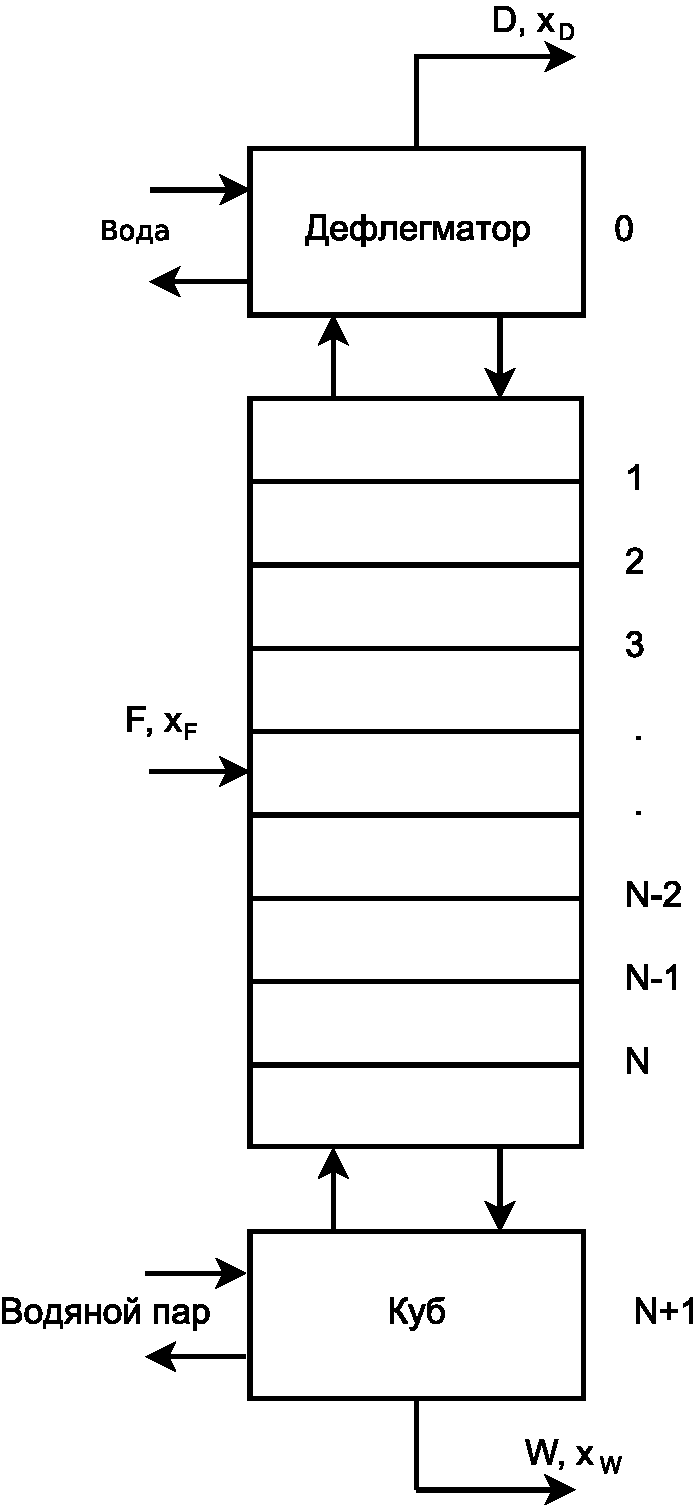
\includegraphics[width=0.48\textwidth]{colomn.pdf}
	\end{center}
	\caption{Схема ректификационной колонны} \label{fig:rect.col}
\end{wrapfigure}
 
Вместе с тем следует отметить, что все названные выше эффекты обычно ускоряют процесс массопереноса. Поэтому при расчете процесса ректификации это, как правило, дает запас производительности и эффективности колонны.

Тарельчатые колонны относятся к аппаратам со ступенчатым контактом фаз и для их расчета используют метод расчета «от тарелки к тарелке». Каждой тарелке присваивают порядковый номер, нумерацию ведут сверху вниз (рисунок \ref{fig:rect.col}). При расчете ректификационной колонны необходимо учитывать дефлегматор и кипятильник, которым также присваивают номера: дефлегматору --- нулевой; кипятильнику --- $N + 1$. При рассмотрении ректификационных колонн для разделения бинарной смеси применим однонаправленный расчет (снизу вверх или сверху вниз) колонны.


На первом этапе оценки возможности проведения процесса разделения смеси используется метод теоретической тарелки. Полученные при этом результаты позволяют дать предварительную оценку необходимого количества ступеней разделения и определить основные режимные параметры процесса давление, флегмовое число и т.д., в последующем эти результаты уточняются. 

При рассмотрении ректификационной колонны в рамках метода теоретической тарелки, основное влияние на точность расчета оказывает правильность определения условий фазового равновесия пар – жидкость. 

Условия равновесия двух фаз $n$~-- компонентной системы, когда температура в каждой фазе одинаковы, определяются следующей системой уравнений:
\begin{equation}
	\left\lbrace 
	\begin{gathered} 
	p^{ж}(T, x_1, x_2, \ldots, x_n-1)=\\=p^{п}(T, y_1, y_2, \ldots, y_n-1)\\
	\mu_k^{ж}(T, x_1, x_2, \ldots, x_n-1)=\\=\mu^{п}_k(T, y_1, y_2, \ldots, y_n-1) 
	\end{gathered} 
	\right.
\end{equation}
где $\mu$ --- химический потенциал, $п$ и $ж$ --- паровая и жидкая фазы, соответственно. Химический потенциал и давление системы определяются следующим образом:
\begin{equation}
	\mu_i(T,x)=\mu_i^0 (T) +RT \ln(\gamma_i x_i)
\end{equation}
\begin{equation}
	p=\sum\limits_{i=1}^{n} p_i= \sum\limits_{i=1}^{n} \gamma_i p_i^0 x_i
\end{equation}

В этом случае для расчета условий фазового равновесия кроме давления паров чистого компонента при заданной температуре $p_i^0(T)$ и идеальногазовой составляющей химического потенциала $\mu_i^0(T)$, необходимо определять коэффициенты активности $\gamma_i$ в зависимости от температуры, давления и состава.

При расчете процессов разделения для упрощения задачи перепад давления (гидравлическое сопротивление) по высоте ректификационной колонны принимают равным нулю. Таким образом, процесс разделения обычно моделируется при фиксированном давлении, а профиль температур по колонне определяется в ходе расчета исходя из состава смеси в колонне. В действительности же, давление в кубе колонне всегда больше чем вверху колонны на величину ее гидравлического сопротивления. 

При расчете условий фазовых равновесий используется концепция избыточной энергии Гиббса, которая заключается в том, что уровень энергии Гиббса для смеси превышает величину характерную для идеального раствора при тех же значениях температуры, давления и состава. Выражения для определения избыточной мольной энергии Гиббса:
\begin{equation}
	G^E=RT(x_1\ln (\gamma_1) +x_2 \ln(\gamma_2))
\end{equation}

Некоторые уравнения для избыточной мольной энергии Гиббса $G^E$ в отличие от уравнения Маргулеса содержат температуру в явном виде (NRTL и др.) \cite{rid1982,yelles1989}. Однако из этого вовсе не следует, что константы таких уравнений не зависят от температуры. Приводимая явная температурная зависимость --- всего лишь приближение и ни в коем случае такие уравнения для $G^E$ не являются точными.

Кроме того, основное влияние температуры на равновесие пар~-- жидкость оказывается через давление паров чистых компонентов $p^0(T)$. Коэффициенты активности зависят как от температуры, так и от состава, и температурную зависимость коэффициентов активности можно считать слабо выраженной по сравнению с зависимостью давлений паров чистых жидкостей от температуры. Для типовой смеси подъем температуры на 10$\mathrm{^\circ}C$ приводит к возрастанию давлений паров чистых жидкостей в $1.5 - 2$ раза, а изменение коэффициентов активности составит скорей несколько процентов, т.е., величину, которая часто меньше погрешности эксперимента. Таким образом, если не происходит сильного изменения температуры, часто при расчетах равновесия пар~-- жидкость можно пренебречь влиянием температуры на $G^E$.
 
Таким образом, на достоверность моделирования процесса разделения значительное влияние оказывает правильность определения температуры на каждой ступени контакта фаз.

В общем виде математическая модель процесса разделения, протекающая на N--ой ступени (рисунок \ref{fig:rect.col}), запишется в виде:
\begin{equation} \label{eq:rect.equation}
\left\lbrace 
\begin{gathered} 
E=\dfrac{y_{N+1}-y_{N}}{y_{N+1}-y^*}\\
L(x_{N-1}-x_N)=G(y_N-y_{N+1})
\end{gathered} 
\right.
\end{equation}
где $Е$ --- коэффициент полезного действия (или эффективности) по Мэрфи; $L$, $G$ --- мольные расходы жидкой и паровой фаз по высоте колонны, соответственно; $y^*$ – равновесная концентрация в паровой фазе. Данную модель необходимо дополнить уравнением, определяющим равновесные концентрации компонентов в паре:
\begin{equation}
	y_i^*=\dfrac{p_i^0 \gamma_i x_i}{p}
\end{equation}
и выражением для определения давления паров чистых компонентов $p^0(Т)$ и коэффициентов активности $\gamma(x,T)$.

Для решения системы уравнений \eqref{eq:rect.equation} необходимо определить мольные расходы паровой и жидкой фаз по высоте колонны. Для этого первоначально необходимо из материального баланса определить расходы дистиллята $D$ и кубового остатка $W$:
\begin{equation}
	W = \dfrac{F (x_D - x_F)}{x_D - x_W},
\end{equation}
\begin{equation}
	D = F - W,
\end{equation}
индексами $D$, $W$, $F$ обозначены составы дистиллята, кубового остатка и исходной смеси соответственно. 

Рабочее флегмовое число определяется исходя из минимального флегмового числа:
\begin{equation}
	R_{min}  = \dfrac{x_D - y^*_F}{y^*_F - x_F}.
\end{equation}
Предложено несколько вариантов определения флегмового числа, исходя из минимизации затрат на проведение процесса. В данной лабораторной работе предлагается пользоваться заданным значением коэффициента избытка флегмы $\beta$:
\begin{equation} 
	R = R_{min} \beta
\end{equation}
Всю колонну можно разбить на 2 части, разделяемые тарелкой питания. В верхней части поток жидкой фазы будет равен:
\begin{equation}
	L_{u} = D R \dfrac{M^x_u}{M_D},
\end{equation}
в нижней:
\begin{equation}
	L_{d} = DR \dfrac{M^x_d}{M_D} + F \dfrac{M^x_d}{M_F}
\end{equation}
В верхней части поток газовой фазы равен:
\begin{equation}
G_u = D(R+1)\dfrac{M^y_u}{M_D},
\end{equation}
в нижней:
\begin{equation}
G_d = D(R+1)\dfrac{M^y_d}{M_D},
\end{equation}
где $M$ --- молярные массы смеси, нижние индексы $u$ и $d$ обозначают средние значения в врхней и нижней части соответственно, верхние индексы $x$ и $y$ обозначают фазу.



\subsubsection*{Вопросы для самоконтроля}
\begin{enumerate}
\item Что понимается под процессом ректификации, в чем его отличие от дистилляции? 
\item Что такое флегмовое число и каково его влияние на процесс разделения?
\item Что называется теоретической тарелкой?
\item Что такое эффективность по Мэрфри и как она влияет на высоту ректификационной колонны?
\item Какие допущения используются при расчете процесса ректификации?
\end{enumerate}


\subsubsection{Пример задания}
Используя язык программирования MathCad провести расчеты простой тарельчатой ректификационной колонны непрерывного действия, предназначенной для разделения $F = 5$ т/ч исходной бинарной смеси, содержащей  $x_F = 34$~\% масс. низкокипящего компонента. Разделение проводится при атмосферном давлении. Исходная смесь поступает в аппарат при температуре кипения. Требуемый состав дистиллята $x_D = 91$~\% масс, куба --- $x_W = 0.5$~\%. Коэффициент избытка флегмы $\beta = 1.25$. КПД тарелок $E = 0.7$.
Для расчета использовать метод расчета от тарелки к тарелке. Допущения при расчете:
\begin{enumerate}
	\item куб колонны --- полный испаритель;
	\item дефлегматор --- полный конденсатор.
\end{enumerate}

В качестве исходной смеси принять смесь согласно своему варианту из лабораторной работы 5, и использовать полученные там функции для составов паровой и жидкой фаз.




\addcontentsline{toc}{section}{\bibname}
\bibliographystyle{utf8gost71u}  
\bibliography{lib.bib}
\end{document}
